\documentclass[a4paper]{article}

\usepackage[utf8]{inputenc}
\usepackage{graphicx}
\usepackage{amstext,amsmath,amsxtra,amssymb,latexsym,amscd,amsthm}
\usepackage{bm}
\usepackage{bbm}
\usepackage{indentfirst}
\usepackage[mathscr]{eucal}
\usepackage{graphicx}
\usepackage{enumitem}

\usepackage{geometry}
\geometry{margin=1in}

\usepackage{float}
% \usepackage{floatrow}
\usepackage{layout}
\usepackage{longtable}
\usepackage{multirow}
\usepackage{caption}
\usepackage{authblk}

\usepackage{mathrsfs}
\setlength{\parindent}{0pt} \setlength{\parskip}{5pt}
\renewcommand{\baselinestretch}{1.0}
\usepackage{fancyhdr}

\usepackage[framed,numbered]{matlab-prettifier}
\usepackage{listings}             % Include the listings-package
\lstset{language=Matlab}
\lstdefinestyle{myCustomMatlabStyle}{
    language=Matlab,
    numbers=left,
    stepnumber=1,
    numbersep=10pt,
    tabsize=4,
    showspaces=false,
    showstringspaces=false,
}
\lstset{basicstyle=\tiny,style=myCustomMatlabStyle}

\usepackage[normalem]{ulem}
\usepackage{url}
\usepackage{subfig}
\usepackage{hyperref}


\usepackage{algorithm2e}
\RestyleAlgo{boxed}
\RestyleAlgo{boxruled}



\usepackage{tikz}
\usetikzlibrary{matrix,shapes,arrows,positioning,chains}
% Define block styles
\tikzset{
    block/.style={
            rectangle,
            draw,
            text width=12em,
            text centered,
        },
    decision/.style={
            rectangle,
            draw,
            text width=12em,
            text centered,
            rounded corners
        },
    cloud/.style={
            draw,
            ellipse,
            minimum height=2em
        },
    descr/.style={
            fill=white,
            inner sep=2.5pt
        },
    connector/.style={
            -latex,
            font=\scriptsize
        },
    rectangle connector/.style={
            connector,
            to path={(\tikztostart) -- ++(#1,0pt) \tikztonodes |- (\tikztotarget) },
            pos=0.5
        },
    rectangle connector/.default=-2cm,
    straight connector/.style={
            connector,
            to path=--(\tikztotarget) \tikztonodes
        }
}

%% Math macros


% Matrix notation
\renewcommand{\vec}[1]{\ensuremath{\bm{#1}}}
\newcommand{\mat}[1]{\ensuremath{\mathbf{#1}}}
\newcommand{\transpose}{\mathsf{T}}

% Interface notations
\newcommand{\jump}[1]{\ensuremath{[\![#1]\!]}}
\newcommand{\avg}[1]{\ensuremath{\langle#1\rangle}}

% Constants
\newcommand{\imunit}{\ensuremath{\underline{\mathrm{i}}}}
\newcommand{\euler}{\ensuremath{\mathrm{e}}}

% Intrinsic diffusion coefficient
\newcommand{\Dintr}{\ensuremath{\mathcal{D}_0}}

% Physical units in dMRI
% \newcommand{\munit}{\ensuremath{\mathrm{A/m}}} % Magnetization
% \newcommand{\sunit}{\ensuremath{\mathrm{A m^2}}} % Signal
\newcommand{\munit}{\ensuremath{}} % Magnetization
\newcommand{\sunit}{\ensuremath{\mathrm{}}} % Signal
\newcommand{\dunit}{\ensuremath{\mathrm{mm^2/s}}} % Diffusivity
\newcommand{\bunit}{\ensuremath{\mathrm{s}/\text{mm}^2}} % B-value
\newcommand{\tunit}{\ensuremath{\mathrm{ms}}} % Time
\newcommand{\kunit}{\ensuremath{\mathrm{m/s}}} % Permeability
\newcommand{\gunit}{\ensuremath{\mathrm{T/m}}} % Gradient amplitude
\newcommand{\lunit}{\ensuremath{\mathrm{\mu m}}} % Length
\newcommand{\qunit}{\ensuremath{\mathrm{(\mu s \mu m)^{-1}}}} % Q-value

% Step sizes
\newcommand{\dx}{\ensuremath{{\Delta x}}}
\newcommand{\dy}{\ensuremath{{\Delta y}}}
\newcommand{\dz}{\ensuremath{{\Delta z}}}
\newcommand{\dt}{\ensuremath{{\Delta t}}}

% Fixed length vectors
\newcommand{\vtwo}[2]{\ensuremath{\begin{bmatrix}#1\\#2\end{bmatrix}}}
\newcommand{\vthree}[3]{\ensuremath{\begin{bmatrix}#1\\#2\\#3\end{bmatrix}}}

% Bold units
\newcommand{\bx}{\ensuremath{{\bm{x}}}}
\newcommand{\by}{\ensuremath{{\bm{y}}}}
\newcommand{\bz}{\ensuremath{{\bm{z}}}}
\newcommand{\br}{\ensuremath{{\bm{r}}}}
\newcommand{\bs}{\ensuremath{{\bm{s}}}}
\newcommand{\bg}{\ensuremath{{\bm{g}}}}
\newcommand{\ba}{\ensuremath{{\bm{a}}}}
\newcommand{\bM}{\ensuremath{{\bm{M}}}}
\newcommand{\bk}{\ensuremath{{\bm{k}}}}
\newcommand{\bG}{\ensuremath{{\bm{G}}}}
\newcommand{\bL}{\ensuremath{{\bm{L}}}}
\newcommand{\bD}{\ensuremath{{\bm{D}}}}
\newcommand{\bn}{\ensuremath{{\bm{n}}}}
\newcommand{\bq}{\ensuremath{{\bm{q}}}}
\newcommand{\bv}{\ensuremath{{\bm{v}}}}
\newcommand{\bnu}{\ensuremath{{\bm{\nu}}}}
\newcommand{\bug}{\ensuremath{\bm{u}_{\bm{g}}}}
\newcommand{\bua}{\ensuremath{\bm{u}_{\bm{a}}}}
\newcommand{\bbd}[1]{\ensuremath{\bm{#1}}}
\newcommand{\bmhat}{\ensuremath{{\bm{\widehat{m}}}}}

% Short forms
\newcommand{\eps}{\ensuremath{\epsilon}}
\newcommand{\R}{\ensuremath{\mathbb{R}}}
\newcommand{\rtwo}{\ensuremath{{\mathbb{R}}^2}}
\newcommand{\rthree}{\ensuremath{{\mathbb{R}}^3}}
\newcommand{\rd}{\ensuremath{{\mathbb{R}}^d}}

% Math environments
\newcommand{\ben}{\begin{equation*}}
        \newcommand{\een}{\end{equation*}}
\newcommand{\be}[1]{\begin{equation} \label{#1}}
        \newcommand{\ee}{\end{equation}}
\newcommand{\eqn}[1]{(\ref{eqn:#1})}

% Kernels
\newcommand{\kernel}[2]{\ensuremath{{\frac{e^{-{\|#1\|^2}/{4#2}}}{(4\pi #2)^{\frac{d}{2}}}}}}
\newcommand{\kerneltext}[2]{\ensuremath{{{e^{-{\|#1\|^2}/{4#2}}}/{(4\pi #2)^{\frac{d}{2}}}}}}

% Fourier transform
\newcommand{\fourier}[1]{\ensuremath{\int \limits_{\rd}e^{i \bs \cdot \bx}  #1 \, d\bx}}
\newcommand{\invf}[1]{\ensuremath{\frac{1}{(2\pi)^d} \int \limits_{\rd} e^{-i \bs \cdot \bx} #1 \, d\bs }}
\newcommand{\invfapprox}[1]{\ensuremath{\frac{1}{(2\pi)^d} \int \limits_{\|\bs\| \leq p} e^{-i \bs \cdot \bx} #1 \, d\bs }}

% Review
%\newcommand{\question}[1]{{\bf #1}}
\newcommand{\ignore}[1]{}

% Scientific notation
\newcommand{\e}[1]{\ensuremath{\times 10^{#1}}}

% Fractions
\newcommand{\half}{\ensuremath{\frac{1}{2}}}
\newcommand{\threehalf}{\ensuremath{\frac{3}{2}}}
\newcommand\fr[2]{{\textstyle\frac{#1}{#2}}}

% Partial derivatives
\newcommand{\pd}[2]{\ensuremath{\frac{\partial #1}{\partial #2}}}
\newcommand{\pdtwo}[2]{\ensuremath{\frac{\partial^2 #1}{\partial #2^2}}}

\newcommand{\HRule}{\rule{\linewidth}{0.5mm}}
\newcommand\etc{\textsl{etc}}
\newcommand\eg{\textsl{eg.}\ }
\newcommand\etal{\textsl{et al.}}
\newcommand\Quote[1]{\lq\textsl{#1}\rq}
%%%%%\soutnew{old text we are removing}{replacement text}
%%%%%\soutnew{}{added text}
%%%%%\soutnew{remove text}{}

%%%%% for reviewers to mark the file
%\newcommand{\soutnew}[2]{\sout{#1} \uwave{#2}}

%%%%% for final latex version generation
\newcommand{\soutnew}[2]{#2}


%%%%\marginparnew{comment to reviewer}
%%%%% for reviewers to mark the file
%\newcommand{\marginparnew}[1]{\marginpar{#1}}

%%%%% for final latex version generation
\newcommand{\marginparnew}[1]{}

\graphicspath{{figures/}}



\title{SpinDoctor User Guide}
\author{Syver Døving Agdestein, Van-Dang Nguyen, Chengran Fang, Demian Wassermann, Jing-Rebecca Li}
\affil{\textbf{INRIA-Saclay, CMAP, 91120 Palaiseau, France}}
\date{\today}



\begin{document}


\textbf{\huge SpinDoctor User Guide}

Updated \today

The user is advised to download the latest version of the User Guide from \url{https://github.com/jingrebeccali/SpinDoctor}.




\setcounter{tocdepth}{2}
\tableofcontents
\newpage






\section{Introduction}
\label{sec:introduction}

The MATLAB Toolbox SpinDoctor \cite{lid} is a simulation pipeline that
\begin{enumerate}
    \item allows the user to define a geometrical configuration;
    \item solves the Bloch-Torrey equation in that geometrical configuration;
    \item fits the apparent diffusion coefficient from the simulated signal.
\end{enumerate}
It includes two other methods for calculating the apparent diffusion coefficient:
\begin{enumerate}
    \item The first is a homogenized apparent diffusion coefficient mathematical model, which was obtained recently using homogenization techniques on the Bloch-Torrey equation. In the homogenized model, the apparent diffusion coefficient of a geometrical configuration can be computed after solving a diffusion equation subject to a time-dependent Neumann boundary condition, under the assumption of negligible water exchange between compartments.
    \item The second module computes the short time approximation formula for the apparent diffusion coefficient. The short time approximation implemented in SpinDoctor includes a recent generalization of this formula to account for finite pulse duration in the pulsed gradient spin echo.
\end{enumerate}
Both of these two apparent diffusion coefficient calculations are sensitive to the diffusion-encoding gradient direction, unlike many previous works where the anisotropy is neglected in analytical model development.

In nutshell, SpinDoctor
\begin{enumerate}
    \item solves the Bloch-Torrey equation in three dimensions to obtain the diffusion magnetic resonance imaging signal;
    \item robustly fits the diffusion magnetic resonance imaging signal to obtain the apparent diffusion coefficient;
    \item solves the homogenized apparent diffusion coefficient model in three dimensions to obtain the	apparent diffusion coefficient;
    \item computes the short-time approximation of the apparent diffusion coefficient;
    \item computes useful geometrical quantities such as the compartment volumes and surface areas;
    \item allows permeable membranes for the Bloch-Torrey equation (the homogenized apparent diffusion coefficient model assumes negligible permeability);
    \item displays the gradient-direction dependent signal or apparent diffusion coefficient in three dimensions.
\end{enumerate}

SpinDoctor provides the following built-in functionalities:
\begin{enumerate}
    \item the placement of non-overlapping spherical cells (with an optional nucleus) of different radii close to each other;
    \item the placement of non-overlapping cylindrical cells (with an optional myelin layer) of different radii close to each other in a canonical configuration where they are parallel to the $z$-axis;
    \item the inclusion of an extra-cellular space that is enclosed either
          \begin{enumerate}
              \item in a tight wrapping around the cells; or
              \item in a rectangular box.
          \end{enumerate}
    \item the deformation of the canonical configuration by bending and twisting.
\end{enumerate}

Built-in diffusion-encoding pulse sequences include
\begin{enumerate}
    \item the Pulsed Gradient Spin Echo;
    \item the Oscillating Gradient Spin Echo (cos- and sin- type gradients);
    \item the Double Pulsed Gradient Spin Echo.
\end{enumerate}
There is also support for custom diffusion-encoding pulse sequences.

SpinDoctor uses the following methods:
\begin{enumerate}
    \item it generates a good quality surface triangulation of the user specified geometrical configuration by calling built-in MATLAB computational geometry functions;
    \item it creates a good quality tetrahedra finite elements mesh from the above surface triangulation by calling Tetgen \cite{tetgen}, an external package (executable files are included in the Toolbox package);
    \item it constructs finite element matrices for linear finite elements on tetrahedra (P1 finite elements) using routines from \cite{RahmanValdman2013};
    \item it adds additional degrees of freedom on the compartment interfaces to allow permeability conditions for the	Bloch-Torrey equation using the formalism in \cite{Nguyen2014d};
    \item it solves the semi-discretized finite elements method equations by calling built-in MATLAB routines for solving ordinary differential equations.
\end{enumerate}



%%
%% Start line numbering here if you want
%%
% \linenumbers

%% main text
\section*{Abbreviations}
The following abbreviations are used throughout the text and code:
\begin{itemize}
    \item ADC, Apparent Diffusion Coefficient;
    \item BT, Bloch-Torrey;
    \item BTPDE, Bloch-Torrey PDE;
    \item DMRI, Diffusion MRI;
    \item ECS, Extra-Cellular Space;
    \item FEM, Finite Element Method;
    \item FPK, Finite Pulse Karger model;
    \item HADC, homogenized ADC;
    \item HARDI, High Angular Resolution Diffusion Imaging;
    \item MF, Matrix Formalism;
    \item MRI, Magnetic Resonance Imaging;
    \item ODE, Ordinary Differential Equation;
    \item OGSE, Oscillating Gradient Spin Echo;
    \item PDE, Partial Differential Equation;
    \item PGSE, Pulsed-Gradient Spin Echo;
    \item STA, Short Time Approximation.
\end{itemize}





\section{Installation}

The SpinDoctor Toolbox has been tested with MATLAB R2018a-R2021a. The user is advised to download the latest version of the User Guide from \url{https://github.com/jingrebeccali/SpinDoctor}. Examples of drivers that run some typical simulations also can be found there.

The SpinDoctor Toolbox has been developed in the MATLAB R2020b and require no additional MATLAB toolboxes. SpinDoctor has support for parallel computations, if the MATLAB Parallel Computing Toolbox is available.


\section{Mathematical background}

Consider a connected three-dimensional domain $\Omega = \bigcup_{i = 1}^{N_\text{cmpt}} \Omega_i \subset \mathbb{R}^3$ consisting of $N_\text{cmpt}$ compartments $\{\Omega_i\}_{1 \leq i \leq N_\text{cmpt}}$. The permeable interface between two compartments is denoted by $\Gamma_{i j} = \Omega_i \cap \Omega_j$ for $i \neq j$, $(i, j) \in \{1, \dots, N_\text{cmpt}\}^2$. For $i = j$, we let $\Gamma_{ii} = \emptyset$ for the ease of notation. Finally, let $\partial \Omega$ denote the outer boundary of the domain, and $\Gamma_i = \Omega_i \cap \partial \Omega$ its restriction to $\Omega_i$. Note that for compartments that do not touch, we have $\Gamma_{i j} = \emptyset$. Similarly, we have $\Gamma_i = \emptyset$ for compartments that do not touch the outer boundary.


\subsection{Bloch-Torrey PDE}

In diffusion MRI, a time-varying magnetic field gradient is applied to the tissue to encode water diffusion. Denoting the effective time profile of the diffusion-encoding magnetic field gradient by $f : [0, T_\text{echo}] \to [-1, 1]$, and letting the vector $\vec{g}$ contain the amplitude and direction information of the magnetic field gradient, the complex transverse water proton magnetization in the rotating frame satisfies the Bloch-Torrey PDE in each compartment $\Omega_i$, $1 \leq i \leq N_\text{cmpt}$:
\begin{equation} \label{eq:btpde}
    \frac{\partial}{\partial t} M_i(\vec{x},t) = -\left(-\nabla \cdot \mat{D}_i \nabla + \frac{1}{T_{2,i}} + \imunit \gamma f(t) \vec{g} \cdot \vec{x}\right) M_i(\vec{x}, t), \quad (\vec{x}, t) \in \Omega_i \times[0, T_\text{echo}],
\end{equation}
where $\gamma = 2.67513\times 10^8 \, \mathrm{rad \, s^{-1} T^{-1}}$ is the gyromagnetic ratio of the water proton and $\imunit$ is the imaginary unit. For each compartment $\Omega_i$, $1 \leq i \leq N_\text{cmpt}$, $\mat{D}_i$ is the intrinsic diffusion tensor, $T_{2,i}$ is the $T_2$-relaxation time and $M_i$ is the magnetization. The diffusion tensors are assumed to be symmetric positive definite, and the relaxation times positive. We also allow for $T_{2,i} = \infty$, in which case the corresponding term is removed from the equation.

The magnetization is a function of position $\vec{x}$ and time $t$, and depends on the diffusion gradient vector $\vec{g}$ and the time profile $f$. The initial spin density is given by
\begin{equation}
    M_i(\vec{x}, 0) = \rho_i \in \mathbb{C}, \quad 1 \leq i \leq N_\text{cmpt}.
\end{equation}

The outer boundary conditions for the BTPDE are given by
\begin{equation}
    \mat{D}_i \nabla M_i(\vec{x}, t) \cdot \vec{n}_i(\vec{x}) = -\kappa_i M_i(\vec{x}, t), \quad \vec{x} \in \Gamma_i, \quad i \in \{1, \dots, N_\text{cmpt}\},
\end{equation}
where $\vec{n}_i$ is the unit outward pointing normal vector of compartment $\Omega_i$ and $\kappa_i$ is an outer boundary relaxation coefficient for $\Omega_i$. Note that we may have $\Gamma_i = \emptyset$, as all the compartments do not necessarily touch the outer boundary.

The BTPDE also needs to be supplemented by interface conditions. We recall that the interface between $\Omega_i$ and $\Omega_j$ is $\Gamma_{i j}$. The two interface conditions on $\Gamma_{i j}$ are the flux continuity and a condition that incorporates a permeability coefficient $\kappa_{i j} \geq 0$ across $\Gamma_{i j}$:
\begin{alignat}{3}
    \mat{D}_i \nabla M_i(\vec{x}, t) \cdot \vec{n}_i(\vec{x}) & = -\mat{D}_j \nabla M_j(\vec{x}, t) \cdot \vec{n}_j(\vec{x}), \quad                  &  & \vec{x} \in \Gamma_{i j}, \quad (i, j) \in \{1, \dots, N_\text{cmpt}\}^2, & \\
    \mat{D}_i \nabla M_i(\vec{x}, t) \cdot \vec{n}_i(\vec{x}) & = \kappa_{i j} \left(c_{i j} M_j(\vec{x}, t) - c_{j i} M_i(\vec{x}, t)\right), \quad &  & \vec{x} \in \Gamma_{i j}, \quad (i, j) \in \{1, \dots, N_\text{cmpt}\}^2. &
\end{alignat}
Here, the permeability coefficient characterizes the membrane: $\kappa_{i j} = \kappa_{j i}$. The two weights $c_{i j}$ and $c_{j i}$ account for the spin density equilibrium between the two compartments. These may both be set to $1$, in which case a uniform spin density across compartments is favored in the absence of a gradient. For different initial spin densities $\rho_i$ and $\rho_j$, we also allow for non-symmetrical weights, for example\cite{Lee2021} $c_{i j} = \frac{2 \rho_i}{\rho_i + \rho_j}$ and $c_{j i} = \frac{2 \rho_j}{\rho_i + \rho_j}$. This ensures that the non-uniform intitial spin density is preserved if the gradient $\vec{g}$ is zero, as $c_{i j}$ and $c_{j i}$ are proportional to $\rho_i$ and $\rho_j$ respectively. The normalization coefficient $2 / (\rho_i + \rho_j)$ ensures that $c_{i j} = c_{j i} = 1$ if $\rho_i = \rho_j$.

For the ease of notation, inside volume integrals, we will use the quantities $\mat{D}$, $T_2$, $\rho$, and $M$ (defined almost everywhere):
\begin{equation}
    \forall i \in \{1, \dots, N_\text{cmpt}\} :
    \begin{cases}
        \mat{D}(\vec{x}) = \mat{D}_i, \quad    & \vec{x} \in \Omega_i                                 \\
        T_2(\vec{x}) = T_{2,i}, \quad          & \vec{x} \in \Omega_i                                 \\
        \rho(\vec{x}) = \rho_i, \quad          & \vec{x} \in \Omega_i                                 \\
        M(\vec{x}, t) = M_i(\vec{x}, t), \quad & (\vec{x}, t) \in \Omega_i \times [0, T_\text{echo}].
    \end{cases}
\end{equation}

In Eq. \eqref{eq:btpde}, the minus sign is factored out of right hand side as, with the prescribed boundary conditions, the \emph{Bloch-Torrey operator}, $$-\nabla \cdot \mat{D} \nabla + \frac{1}{T_2} + \imunit \gamma f(t) \vec{g} \cdot \vec{x},$$ has eigenvalues with nonnegative real parts for all $t$, $f$, $\vec{g}$, and positive $T_2$ and \mat{D}.



\subsection{Diffusion MRI model}

The diffusion MRI signal is measured at echo time $t = T_\text{echo}$. This signal is computed as the spatial integral  of the final magnetization $M(\vec{\cdot}, T_\text{echo})$:
\begin{equation}\label{eq:signal}
    S = \int_\Omega M(\vec{x}, T_\text{echo}) \, \mathrm{d} \Omega(\vec{x}),
\end{equation}
and represents the output of the SpinDoctor diffusion MRI model. The model input is the gradient sequence, encoded by the amplitude and direction $\vec{g}$ and effective time profile $f$. Some commonly used time profiles (diffusion-encoding sequences) are:
\begin{enumerate}
    \item The pulsed-gradient spin echo (PGSE) \cite{Stejskal1965} sequence, with two rectangular pulses of duration $\delta$, separated by a time interval $\Delta - \delta$, for which the profile $f(t)$ is
          \begin{equation}\label{eq:pgse}
              f(t) =
              \begin{cases}
                  1, \quad & t_1 \leq t \leq t_1+\delta,            \\
                  -1,
                  \quad    & t_1+\Delta < t \leq t_1+\Delta+\delta, \\
                  0, \quad & \text{otherwise},
              \end{cases}
          \end{equation}
    \item The double pulsed-gradient spin echo (DPGSE) sequence consists of two PGSE sequences separated by a gap $t_\text{pause}$. If $f_{\delta, \Delta}$ is a PGSE sequence with parameters $\delta$ and $\Delta$, the double PGSE sequence $f$ is given by
          \begin{equation}\label{eq:pgse}
              f(t) = f_{\delta, \Delta}(t) + f_{\delta, \Delta}\left(t - (\Delta + \delta + t_\text{pause}) \right).
          \end{equation}
    \item The oscillating gradient spin echo (OGSE) sequence \cite{Callaghan1995,Does2003}	was introduced to reach short diffusion times. An OGSE	sequence usually consists of two oscillating pulses of duration $\delta$, each containing $n$ periods, hence the	frequency is $\omega = n\frac{2\pi}{\delta}$, separated by a time interval $\Delta-\delta$. For a cosine OGSE, the profile $f(t)$ is
          \begin{equation}\label{eq:ogse}
              f(t) =
              \begin{cases}
                  \cos\left(n \frac{2\pi}{\delta} (t - t_1)\right), \quad            & t_1 < t \leq t_1 + \delta,                   \\
                  -\cos\left(n \frac{2 \pi}{\delta} (t - \Delta - t_1)\right), \quad & t_1 + \Delta < t \leq t_1 + \Delta + \delta, \\
                  0, \quad                                                           & \text{otherwise},
              \end{cases}
          \end{equation}
\end{enumerate}
where $t_1$ is the starting time of the first gradient pulse and $t_1 + \Delta \geq T_\text{echo} / 2$. By default, SpinDoctor assumes $t_1 = 0$ and $T_\text{echo} = \Delta + \delta$, meaning that $\rho$ denotes the spin density just before the gradient sequence is applied and $S$ is measured immediately after the end of the pulses. The user can however set up custom sequences taking into account the times before and after the pulses, or model the pulse transitions.

In a dMRI experiment, the pulsed sequence (time profile $f$) is usually fixed, while $\vec{g}$ is varied in amplitude (and possibly also in direction). $S$ is usually plotted against a quantity called the $b$-value. The $b$-value depends on $\vec{g}$ and $f$ and is defined as
\begin{equation*}
    b(\vec{g}, f) = \gamma^2 \|\vec{g}\|^2 \int_0^{T_\text{echo}} \, \mathrm{d}t\left(\int_0^t f(s)\,\mathrm{d}s\right)^2.
\end{equation*}
For PGSE, the b-value is \cite{Stejskal1965}:
\begin{equation}
    b(\vec{g},\delta,\Delta) = \gamma^2 \|\vec{g}\|^2 \delta^2 \left(\Delta - \delta/3\right).
\end{equation}
For the cosine OGSE with \emph{integer}\/ number of periods $n$ in each of the two durations $\delta$, the corresponding $b$-value is \cite{Xu2007}:
\begin{equation}
    b(\vec{g},\delta) = \gamma^2 \|\vec{g}\|^2 \frac{\delta^3}{4 n^2 \pi^2} = \gamma^2 \|\vec{g}\|^2 \frac{\delta}{\omega^2}.
\end{equation}
The reason for these definitions is that in a homogeneous medium, the signal attenuation is $\euler^{-\vec{u}_{\vec{g}}^\transpose \mat{D}_0 \vec{u}_{\vec{g}} b}$, where $\mat{D}$ is the intrinsic diffusion tensor and $\vec{u}_{\vec{g}} = \vec{g} / \|\vec{g}\|$.


\subsection{Fitting the ADC from the dMRI signal}

An important quantity that can be derived from the dMRI signal is the ``Apparent Diffusion Coefficient'' (ADC), which gives an indication of the root mean squared distance travelled by water molecules in the gradient direction $\vec{g}/\|\vec{g}\|$, averaged over all starting positions:
\begin{equation}\label{eq:ADCdef}
    D_\text{ADC} = \left. -\frac{\partial}{\partial b} \log{\frac{S(b)}{S(0)}}\right\vert_{b=0}.
\end{equation}
We numerically compute ADC by a polynomial fit of
$$\log\frac{S(b)}{S_\text{initial}} \approx c_0+c_1b+\dots+c_n b^n,$$
increasing $n$ from 1 onwards until we get the value of $c_1$ to be stable within a numerical tolerance, where $S_\text{initial} = \int_\Omega \rho(\vec{x}) \, \mathrm{d} \Omega(\vec{x})$. The first coefficient is given by $c_0 = \log \frac{S(0)}{S_\text{initial}}$, which is equal to zero if $T_{2,i} = \infty$ for all $i$.

The ADC may be interpreted as a correction to the intrinsic diffusion coefficient, taking into account the deviation from the free diffusion arising from interior interfaces, non-isotropic diffusion, fluid movements etc. For suffiently small b-values, the signal attenuation is given by
\begin{equation*}
    \euler^{-D_\text{ADC} b}.
\end{equation*}

Another quantity of interest is a slight generalization of the ADC---an effective diffusion tensor $\mat{D}_\text{eff}$. The six coefficients of this symmetric positive tensor is fitted to best approximate the following signal attenuation, for all gradients $\vec{g} \in \mathbb{R}^3$:
\begin{equation*}
    \euler^{- \frac{\vec{g}^\transpose \mat{D}_\text{eff} \vec{g}}{\vec{g}^\transpose \vec{g}} b}.
\end{equation*}
The resulting ADC in direction $\vec{g}$ is then given by
\begin{equation}
    D_\text{ADC}(\vec{g}) = \frac{\vec{g}^\transpose \mat{D}_\text{eff} \vec{g}}{\vec{g}^\transpose \vec{g}} = \vec{u}_{\vec{g}}^\transpose \mat{D}_\text{eff} \vec{u}_{\vec{g}}.
\end{equation}


\subsection{HADC model}

In a previous work \cite{schiavi2016}, a PDE model for the time-dependent ADC was obtained starting from the Bloch-Torrey equation, using homogenization techniques. In the case of negligible water exchange between compartments (low permeability), there is no coupling between the compartments, at least to the quadratic order in $\vec{g}$, which is the ADC term. The ADC in compartment $\Omega$ is given by
\begin{equation} \label{eq:hadc}
    D_\text{HADC}(\vec{g}, f) = \vec{u}_{\vec{g}}^\transpose \mat{D} \vec{u}_{\vec{g}} - \frac{\int_0^{T_\text{echo}} F(t) h(t) \, \mathrm{d}t}{\int_0^{T_\text{echo}} F(t)^2 \, \mathrm{d} t} ,
\end{equation}
where $F(t) = \int_0^t f(s) \, \mathrm{d}s,$ and
\begin{equation} \label{eq:hadc_h_def}
    h(t) = \frac{1}{|\Omega|} \int_{\partial \Omega} \omega(\vec{x}, t) \, \vec{u}_{\vec{g}} \cdot \vec{n}(\vec{x}) \, \mathrm{d} \Gamma(\vec{x})
\end{equation}
is a quantity related to the directional gradient of a function $\omega$ that is the solution of the homogeneous diffusion equation with Neumann boundary condition and zero initial condition:
\begin{alignat}{2}
    \frac{\partial}{\partial t} \omega(\vec{x}, t)  & = \nabla \cdot \left(\mat{D} \nabla \omega(\vec{x}, t)\right), \quad &  & (\vec{x}, t) \in \Omega \times [0, T_\text{echo}], \label{eq:hadc_pde} \\
    \omega(\vec{x}, 0)                              & = 0, \quad                                                           &  & \vec{x} \in \Omega, \label{eq:hadc_initial}                            \\
    \mat{D} \nabla \omega(\vec{x}, t) \cdot \vec{n} & = F(t) \mat{D} \vec{u}_{\vec{g}} \cdot \vec{n}, \quad                &  & \vec{x} \in \partial \Omega, \label{eq:hadc_neumann}
\end{alignat}
$\vec{n}$ being the outward normal and $\vec{u}_{\vec{g}}$ the unit gradient direction. The above set of equations, \eqref{eq:hadc}-\eqref{eq:hadc_neumann}, comprise the homogenized model that we call the HADC model.



\subsection{Short diffusion time approximation of the ADC}

A well-known formula for the ADC in the short diffusion time regime is the following short time approximation (STA) \cite{Mitra1992,Mitra1993}:
\begin{equation*}
    D_\text{STA} = \left(1 - \frac{4\sqrt{D_0}}{3 \sqrt{\pi}}\sqrt{\Delta} \frac{{A}}{d\; V} \right) D_0,
\end{equation*}
where $\dfrac{A}{V}$ is the surface to volume ratio, $d$ is the spatial dimension and $D_0 = \vec{u}_{\vec{g}}^\transpose \mat{D} \vec{u}_{\vec{g}}$ is the intrinsic diffusion coefficient in the gradient direction. In the above formula, the pulse duration $\delta$ is assumed to be very small compared to $\Delta$. A recent correction to the above formula \cite{schiavi2016}, taking into account the finite pulse duration $\delta$ and the gradient direction $\vec{u}_{\vec{g}}$, is the following:
\begin{equation}
    D_\text{STA} = \left(1 - \frac{4 \sqrt{D_0}}{3 \sqrt{\pi}}
    C_{\delta,\Delta}
    \frac{A_{\vec{u}_{\vec{g}}}}{V} \right) D_0,
\end{equation}
where
\begin{equation*}
    A_{\vec{u}_{\vec{g}}} = \int_{\partial \Omega} \left(\vec{u}_{\vec{g}} \cdot \vec{n}(\vec{x})\right)^2 \, \mathrm{d} \Gamma(\vec{x}) = \vec{u}_{\vec{g}}^\transpose \mat{N} \vec{u}_{\vec{g}}
\end{equation*}
with $\mat{N} = \int_{\partial \Omega} \vec{n}(\vec{x}) \vec{n}^\transpose\!(\vec{x}) \, \mathrm{d} \Gamma(\vec{x})$ and
\begin{equation*}
    C_{\delta, \Delta} = \dfrac{4}{35}
    \dfrac{\left(\Delta + \delta \right)^{7 / 2}+ \left(\Delta - \delta\right)^{7 / 2} - 2 \left(\delta^{ 7 / 2} + \Delta^{7 / 2} \right)}{\delta^2 \left( \Delta - \delta / 3\right)} = \sqrt{\Delta} \left(1 + \dfrac{1}{3} \dfrac{\delta}{\Delta} - \dfrac{8}{35} \left(\dfrac{\delta}{\Delta}\right)^{3 / 2} + \dots \right).
\end{equation*}
When $\delta \ll \Delta$, the value $C_{\delta, \Delta}$ is approximately $\sqrt{\Delta}$.





\subsection{Matrix Formalism signal representation}

The Matrix Formalism \cite{Callaghan1997,Barzykin1999} representation of the solution to the Bloch-Torrey PDE is based on the generalized Laplace eigenfunctions of the given geometrical configuration. These are the eigenfunctions of the generalized Laplace operator $-\nabla \cdot \mat{D} \nabla$ subject to the same boundary and interface conditions as the BTPDE. It which does not depend on the gradient sequence. The Matrix Formalism truncates the number of Laplace eigenmodes at an acceptable level, by setting a minimum length scale for the eigenfunctions. The gradient sequence dependent Bloch-Torrey operator can then be expressed in the truncated Laplace eigenfunction basis. This allows for a simple analytical expression which approximates the solution to the BTPDE down to an arbitrary length scale.


\subsubsection{Eigenvalue decomposition of the generalized Laplace operator}

Let $\{(\phi, \lambda)\}$ be the $L^2$-normalized eigenfunctions and eigenvalues of the generalized Laplace operator $\nabla \cdot \mat{D} \nabla$, defined almost everywhere on the domain $\Omega = \bigcup_{i = 1}^{N_\text{cmpt}} \Omega_i$. Denoting $\phi^i$ the restriction of $\phi$ to compartment $\Omega_i$, the eigenfunctions respect the following set of equations, for $(i, j) \in \{1, \dots, N_\text{cmpt}\}^2$:
\begin{equation} \label{eq:laplace_eig}
    -\nabla \cdot \mat{D}_i \nabla \phi^i(\vec{x}) = \lambda \phi^i(\vec{x}), \quad \vec{x} \in \Omega_i, \quad i \in \{1, \dots, N_\text{cmpt}\}.
\end{equation}
where the boundary conditions are the same as for the BTPDE:
\begin{alignat}{3}
    \mat{D}_i \nabla \phi^i(\vec{x}) \cdot \vec{n}_i(\vec{x}) & = -\mat{D}_j \nabla \phi^j(\vec{x}) \cdot \vec{n}_j(\vec{x}), \quad                 &  & \vec{x} \in \Gamma_{i j}, \quad (i, j) \in \{1, \dots, N_\text{cmpt}\}^2, &                        \\
    \mat{D}_i \nabla \phi^i(\vec{x}) \cdot \vec{n}_i(\vec{x}) & = \kappa_{i j} \left(c_{i j} \phi^j(\vec{x}) - c_{j i}\phi^i(\vec{x})\right), \quad &  & \vec{x} \in \Gamma_{i j}, \quad (i, j) \in \{1, \dots, N_\text{cmpt}\}^2, &                        \\
    \mat{D}_i \nabla \phi^i(\vec{x}) \cdot \vec{n}_i(\vec{x}) & = -\kappa_i \phi^i(\vec{x}), \quad                                                  &  & \vec{x} \in \Gamma_i, \quad i \in \{1, \dots, N_\text{cmpt}\}.            & \label{eq:lap_neumann}
\end{alignat}

Let the solutions $(\phi, \lambda)$ to the above equations, \eqref{eq:laplace_eig}-\eqref{eq:lap_neumann}, be denoted by $\left\{(\phi_n, \lambda_n)\right\}_{n \in \mathbb{N}^*}$. We assume the non-negative real-valued eigenvalues are ordered in non-decreasing order:
\begin{equation*}
    0 = \lambda_1 \leq \lambda_2 \leq \lambda_3 \leq \dots
\end{equation*}
If the domain $\Omega$ consists of only one contiguous group of compartments connected through a chain of permeable membranes, only the first eigenvalue will be zero, and the corresponding eigenfunction will be the only constant function. If there are $N_\text{group} \geq 2$ groups of connected compartments completely separated by interior hard wall membranes, the first $N_\text{group}$ eigenvalues will be zero:
\begin{equation*}
    0 = \lambda_1 = \dots = \lambda_{N_\text{group}} < \lambda_{N_\text{group} + 1} \leq \dots,
\end{equation*}
and there will be $N_\text{group}$ corresponding groupwise constant eigenfunctions. In the latter case, the equations may be rewritten separately for each connected subdomain to obtain a set of eigenvalues with a multiplicity of one, but the formulation is also valid in the global form with multiple zero eigenvalues. These two formulations will lead to an identical eigenfunction basis (up to a linear combination for the eigenvalues with multiplicity higher than one), where the basis of each subdomain is a subset of the global eigenfunction basis.

Let $\mat{L}$ be the diagonal matrix containing the first $N_\text{eig}$ Laplace eigenvalues:
\begin{equation}
    \mat{L} = \operatorname{diag}(\lambda_1, \lambda_2, \dots, \lambda_{N_\text{eig}})\in \R^{N_\text{eig} \times N_\text{eig}}.
\end{equation}
Then the matrix \mat{L} represents the generalized Laplace operator $-\nabla \cdot \mat{D} \nabla$ in the truncated Laplace eigenfunction basis.


\subsubsection{Bloch-Torrey operator in the Laplace eigenfunction basis}

Let $\mat{A}(\vec{g})$ be the $N_\text{eig} \times N_\text{eig}$ matrix defined by:
\begin{equation}
    \mat{A}(\vec{g}) = g_x \mat{A}^x + g_y \mat{A}^y + g_z \mat{A}^z,
\end{equation}
where $\vec{g} = (g_x, g_y, g_z)^\transpose$ is the gradient vector and $\mat{A}^x$, $\mat{A}^y$, and $\mat{A}^z$ are three symmetric $N_\text{eig} \times N_\text{eig}$ matrices whose entries are the first order moments in the coordinate directions of the product of pairs of eigenfunctions:
\begin{alignat}{3}
    A_{mn}^x & = \int_\Omega x \, \phi_m(\vec{x}) \phi_n(\vec{x}) \, \mathrm{d} \Omega(\vec{x}), \quad &  & (m, n) \in \{1, \dots, N_\text{eig}\}^2, \label{eq:lapeigfirstmm_x} \\
    A_{mn}^y & = \int_\Omega y \, \phi_m(\vec{x}) \phi_n(\vec{x}) \, \mathrm{d} \Omega(\vec{x}), \quad &  & (m, n) \in \{1, \dots, N_\text{eig}\}^2, \label{eq:lapeigfirstmm_y} \\
    A_{mn}^z & = \int_\Omega z \, \phi_m(\vec{x}) \phi_n(\vec{x}) \, \mathrm{d} \Omega(\vec{x}), \quad &  & (m, n) \in \{1, \dots, N_\text{eig}\}^2. \label{eq:lapeigfirstmm_z}
\end{alignat}

Similarly, let \mat{T} be the $N_\text{eig} \times N_\text{eig}$ Laplace relaxation matrix defined by
\begin{equation}
    T_{mn} = \int_\Omega \frac{1}{T_2(\vec{x})} \phi_m(\vec{x}) \phi_n(\vec{x}) \, \mathrm{d} \Omega(\vec{x}), \quad (m,n) \in \{1, \dots, N_\text{eig}\}^2.
\end{equation}

Then the general time dependent Bloch-Torrey operator $$-\nabla \cdot \mat{D} \nabla + \frac{1}{T_2} + \imunit \gamma f(t) \vec{g} \cdot \vec{x}, \quad t \in [0, T_\text{echo}]$$ in the truncated Laplace eigenfunction basis $(\phi_j)_{j = 1, \dots, N_\text{eig}}$ is given by the complex-valued matrix
\begin{equation}
    \mat{K}(\vec{g}, f)(t) = \mat{L} + \mat{T} + \imunit \gamma f(t) \mat{A}(\vec{g}),\quad t \in [0, T_\text{echo}].
\end{equation}

For a piece-wise constant time profile (PGSE, double-PGSE), the Bloch-Torrey operator $$-\nabla \cdot \mat{D} \nabla + \frac{1}{T_2} + \imunit \gamma \vec{g} \cdot \vec{x}$$ is constant. In the truncated Laplace eigenfunction basis, it is given by the complex-valued matrix
\begin{equation}\label{eq:bt_matrix_constant}
    \mat{K}(\vec{g}) = \mat{L} + \mat{T} + \imunit \gamma \mat{A}(\vec{g}).
\end{equation}


\subsubsection{Matrix Formalism approximation}

Denoting $\vec{\phi} = (\phi_1, \dots, \phi_{N_\text{eig}})^\transpose$ the vector of the first $N_\text{eig}$ Laplace eigenfunctions, we may project the solution to to the Bloch-Torrey PDE \eqref{eq:btpde} onto the truncated Laplace eigenfunction basis:
\begin{equation}
    M^\text{MF}(\vec{x}, t) = \vec{\phi}^\transpose\!(\vec{x}) \vec{\nu}(t),
\end{equation}
where the vector of coefficients $\vec{\nu} = (\nu_1, \dots, \nu_{N_\text{eig}})^\transpose : [0, T_\text{echo}] \to \mathbb{C}^{N_\text{eig}}$ is the solution to
\begin{equation}\label{eq:btpde_mf}
    \frac{\mathrm{d} \vec{\nu}}{\mathrm{d} t} = -\mat{K}(\vec{g}, f)(t) \vec{\nu}(t), \quad t\in [0, T_\text{echo}].
\end{equation}
The initial coefficients are given by
\begin{equation}
    \vec{\nu}(0) = \int_\Omega \rho(\vec{x}) \vec{\phi}(\vec{x}) \, \mathrm{d} \Omega(\vec{x}).
\end{equation}
By using a piece-wise constant approximation \cite{Barzykin1999} of the time profile $f$, we obtain
\begin{equation}\label{eq:mf_coefficients}
    \vec{\nu}(T_\text{echo}) \approx \left(\prod_{i = 1}^{N_\text{int}} \euler^{-\delta_i \mat{K}_i}\right) \vec{\nu}(0) = \euler^{-\delta_{N_\text{int}} \mat{K}_{N_\text{int}}} \dots \euler^{-\delta_2 \mat{K}_2} \euler^{-\delta_1 \mat{K}_1} \vec{\nu}(0),
\end{equation}
where $\{I_i\}_{i = 1, \dots, N_\text{int}}$ are intervals such that $[0, T_\text{echo}] = \bigcup_{i = 1}^{N_\text{int}} I_i$, $f(t) = f_i$ for $t \in I_i$, $\delta_i = |I_i|$, and $\mat{K}_i(\vec{g}) = \mat{L} + \imunit \gamma f_i \mat{A}(\vec{g})$. The constants may be computed through quadrature:
\begin{equation}
    f_i = \frac{1}{\delta_i}\int_{I_i} f(t) \, \mathrm{d} t \approx \frac{1}{2} \left(f(\min I_i) + f(\max I_i)\right).
\end{equation}

For the PGSE and double-PGSE sequences, the coefficients of the final magnetization are given by
\begin{equation}\label{eq:mf_coefficients_pgse}
    \vec{\nu}(T_\text{echo}) = \euler^{-\delta\mat{K}^*} \euler^{-(\Delta - \delta)(\mat{L} + \mat{T})} \euler^{-\delta \mat{K}} \vec{\nu}(0)
\end{equation}
and
\begin{equation}\label{eq:mf_coefficients_doublepgse}
    \vec{\nu}(T_\text{echo}) = \euler^{-\delta \mat{K}^*} \euler^{-(\Delta - \delta)(\mat{L} + \mat{T})} \euler^{-\delta \mat{K}} \euler^{-t_\text{pause}(\mat{L} + \mat{T})} \euler^{-\delta \mat{K}^*} \euler^{-(\Delta - \delta)(\mat{L} + \mat{T})} \euler^{-\delta \mat{K}} \vec{\nu}(0)
\end{equation}
respectively. These are the exact solutions to Eq. \eqref{eq:btpde_mf}, although there may still be truncation errors from $N_\text{eig}$. We note that Eq. \eqref{eq:mf_coefficients_pgse} and Eq. \eqref{eq:mf_coefficients_doublepgse} are particular cases of Eq. \eqref{eq:mf_coefficients}, with ($N_\text{int} = 3$, $\mathcal{I}_1 = [0, \delta]$, $\mathcal{I}_2 = [\delta, \Delta]$, $\mathcal{I}_3 = [\Delta, \Delta + \delta]$) and ($N_\text{int} = 7$, $\mathcal{I}_1 = [0, \delta]$, $\mathcal{I}_2 = [\delta, \Delta]$, $\mathcal{I}_3 = [\Delta, \Delta + \delta]$, $\mathcal{I}_4 = [\Delta + \delta, \Delta + \delta + t_\text{pause}]$, $\mathcal{I}_5 = \Delta + \delta + t_\text{pause} + \mathcal{I}_1$, $\mathcal{I}_6 = \Delta + \delta + t_\text{pause} + \mathcal{I}_2$, $\mathcal{I}_7 = \Delta + \delta + t_\text{pause} + \mathcal{I}_3$) respectively.

The notation $^{*}$ denotes the matrix complex conjugate transpose. In order to calculate the non-diagonal matrix exponential $\euler^{-\delta \mat{K}}$ and its conjugate $\euler^{-\delta \mat{K}^*}=\left(\euler^{-\delta \mat{K}}\right)^*$, the scaling and squaring method \cite{Higham2005,Mohy2009} is used (the built-in matrix exponential function in MATLAB, \verb+expm+, is called). For large $N_\text{eig}$ or many gradient sequences $(\vec{g}, f)$, it may also be beneficial to approximate each consecutive vector $\vec{\nu}$ without explicitly computing the matrix exponentials at all, by computing the action of the matrix exponentials on the three successive vectors without computing the matrix exponentials themselves\cite{Mohy2011}. This approach may be used in a future version of SpinDoctor, in particular for other sequences than PGSE. However, for the purpose of theoretical analysis, we may explicitly diagonalize the matrix $\mat{K}(\vec{g})$:
\begin{equation}\label{eq:bt_matrix}
    \mat{K}(\vec{g}) = \mat{V} \mat{B} \mat{V}^{-1},
\end{equation}
where $\mat{V}$ has the eigenvectors in the columns and $\mat{B}$ has the eigenvalues on the diagonal. Then $\euler^{-\delta\mat{K}} = \mat{V} \euler^{-\delta \mat{B}} \mat{V}^{-1}$ and $\euler^{-\delta\mat{K}^*} = \left(\mat{V}^{-1}\right)^{*} \euler^{-\delta \mat{B}^{*}} \mat{V}^{*}$.

The signal is given by
\begin{equation}
    S^\text{MF}(f, \vec{g}) = \vec{\nu}^\transpose\!(T_\text{echo}) \int_\Omega \vec{\phi}(\vec{x}) \, \mathrm{d} \Omega(\vec{x}).
\end{equation}




\subsubsection{Apparent diffusion coefficient}

From the Matrix Formalism signal, the analytical expression of its ADC for a gradient direction given by a unit vector $\vec{u}_{\vec{g}}$ and a sequence $f$ is the following:
\begin{equation*} \label{eq:mf_adc}
    D^\text{MF}(\vec{u}_{\vec{g}}, f) = \frac{1}{|\Omega|} \sum_{n = 1}^{N_\text{eig}} (\vec{u}_{\vec{g}} \cdot \vec{a}_n)^2 \lambda_n \frac{\int_0^{T_\text{echo}} F(t) \int_0^t \euler^{-\lambda_n(t - s)} f(s) \, \mathrm{d} s \, \mathrm{d} t}{ \int_0^{T_\text{echo}} F^2(t) \, \mathrm{d} t},
\end{equation*}
where the coefficients of the three-row matrix $\mat{a} = (\vec{a}_1^, \dots, \vec{a}_{N_\text{eig}}) \in \mathbb{R}^{3 \times N_\text{eig}}$ are given by
\begin{equation}
    \begin{split}
        a_n^x & = \int_{\Omega} x \phi_n(\vec{x}) \, \mathrm{d} \Omega(\vec{x}), \\
        a_n^y & = \int_{\Omega} y \phi_n(\vec{x}) \, \mathrm{d} \Omega(\vec{x}), \\
        a_n^z & = \int_{\Omega} z \phi_n(\vec{x}) \, \mathrm{d} \Omega(\vec{x}),
    \end{split}
    \quad n \in \{1, \dots, N_\text{eig}\}.
\end{equation}

To clarify the relationship between the ADC and the diffusion encoding direction $\vec{u}_{\vec{g}}$, we rewrite the Matrix Formalism ADC as
\begin{equation}
    D^\text{MF}(\vec{u}_{\vec{g}}, f) = \vec{u}_{\vec{g}}^\transpose \mat{D}^{\text{MF}}(f) \vec{u}_{\vec{g}},
\end{equation}
where the Matrix Formalism effective diffusion tensor is given by
\begin{align}
    \label{eq:dmf}
    \mat{D}^{\text{MF}}(f) = \frac{1}{|\Omega|} \sum_{n = 1}^{N_\text{eig}} j_n(f) \vec{a}_n \vec{a}_n^\transpose = \frac{1}{|\Omega|} \mat{a} \mat{j}(f) \mat{a}^\transpose,
\end{align}
with $\mat{j}(f) = \operatorname{diag}\left(j_1(f), \dots, j_{N_\text{eig}}(f)\right) \in \mathbb{R}^{N_\text{eig} \times N_\text{eig}}$ depending on $f$:
\begin{equation}
    j_n(f) = \lambda_n \frac{\int_0^{T_\text{echo}} F(t) \int_0^t e^{-\lambda_n(t - s)} f(s) \, \mathrm{d} s \, \mathrm{d} t}{\int_0^{T_\text{echo}} F^2(t) \, \mathrm{d} t}, \quad n \in \{1, \dots, N_\text{eig}\}.
\end{equation}

In the case of a constant initial spin density $\rho$, we also allow for computing the Matrix Formalism Gaussian Approximation (MFGA) signal, given as
\begin{equation}\label{eq:sig_mfga}
    S^{\text{MFGA}}(\vec{g},f) = \rho|\Omega| \exp\left(-\vec{u}_{\vec{g}}^\transpose \mat{D}^{\text{MF}}(f)\vec{u}_{\vec{g}} \; b(\|\vec{g}\|,f)\right) \quad \vec{u}_{\vec{g}} = \frac{\vec{g}}{\|\vec{g\|}}.
\end{equation}



\subsubsection{Eigenfunction length scale and orientation}

On a line segment of length $L$ and diffusivity $D_0$, the eigenvalues $(\lambda_1, \lambda_2, \dots)$ of the Laplace operator with Neumann boundary conditions are
\begin{equation}
    \lambda_n = \left(\frac{\pi (n - 1)}{L}\right)^2 D_0, \quad n = 1, 2, \dots
\end{equation}
To make the link between the computed eigenvalue and the spatial scale of the eigenmode, we will convert the computed $\lambda_n$ into a length scale:
\begin{equation} \label{eq:lap_eig_lscale}
    \ell(\lambda) =
    \begin{cases}
        + \infty, \quad                                & \lambda = 0, \\
        \pi \sqrt{\frac{\bar{\sigma}}{\lambda}}, \quad & \lambda > 0,
    \end{cases}
\end{equation}
and characterize the computed eigenmode by $\ell(\lambda_n)$ instead of $\lambda_n$. The reference diffusivity $\bar{\sigma}$ is taken as a volume weighted mean of the trace average (spherical part) of $(\mat{D}_i)_{1 \leq i \leq N_\text{cmpt}}$:
\begin{equation}
    \bar{\sigma} = \frac{1}{|\Omega|} \int_\Omega \frac{1}{3}\operatorname{tr} \mat{D}(\vec{x}) \, \mathrm{d} \Omega(\vec{x}).
\end{equation}

To characterize the directional contribution of the eigenmode we use the fact that its contribution to the ADC in the direction $\vec{u}_{\vec{g}}$ is $j_n(f) (\vec{u}_{\vec{g}} \cdot \vec{a}_n)^2$. We thus call $\vec{a}_n = (a_n^x, a_n^y, a_n^z)^\transpose$ the ``diffusion direction'' of the $n$th eigenmode. We remind that the three components of $\vec{a}_n$ are the first moments in the 3 canonical basis directions of the associated eigenfunction.



\subsection{Finite element discretization}

In SpinDoctor, the finite element mesh generation is performed using an external package called Tetgen\cite{tetgen}. Each finite element mesh consists of
\begin{enumerate}
    \item a list of $N_\text{node}$ nodes in three dimensions: $(\vec{q}_1, \dots, \vec{q}_{N_\text{node}}) = (\vec{q}^x, \vec{q}^y, \vec{q}^z)^\transpose \in \R^{3 \times N_\text{node}}$;
    \item a list of $N_\text{element}$ tetrahedral elements ($4 \times N_\text{element}$ indices referencing the nodes).
\end{enumerate}

The list of nodes includes double nodes that are placed at the interfaces between compartments connected by permeable membranes. This allows for representing discontinuous magnetization fields $M_i$ and $M_j$ (or $\phi^i$ and $\phi^j$) on the same boundary $\Gamma_{i j}$. To distinguish between the different compartments, let $\{1, \dots, N_\text{node}\} = \bigcup_{i = 1}^{N_\text{cmpt}} \mathcal{I}_i$ with $\mathcal{I}_i \cap \mathcal{I}_j = \emptyset$ for $i \neq j$. The set $\mathcal{I}_i$ contains the indices of the nodes representing compartment $\Omega_i$, including interface nodes.  In the adjacent compartments, the corresponding interface nodes will have different indices, distinct from $\mathcal{I}_i$.

In SpinDoctor\cite{lid}, the finite element space is the space of compartment-wise continuous piecewise linear functions on tetrahedral elements in three dimensions. This space has a set of basis functions whose number is exactly the number of finite element nodes (including double nodes), and that are defined on the entire domain $\Omega$:
\begin{equation*}
    \varphi_k : \Omega \to [0, 1], \quad k \in \{1, \dots, N_\text{node}\}.
\end{equation*}
Let the finite element nodes be denoted by $\vec{q}_1, \dots, \vec{q}_{N_\text{node}}$. The basis function $\varphi_k$, $k \in \mathcal{I}_i$, is a piece-wise linear function, non-zero on the tetrahedra of $\Omega_i$ that touch the node $\vec{q}_k$, and zero on all other tetrahedra (including tetrahedra of other compartments different than $\Omega_i$ that do touch $\vec{q}_k$). At the interface $\Gamma_{i j}$ between two compartments, the value of $\varphi_k$ is set to be the value it has inside its own compartment, distinct from that of the adjacent compartment. On a tetrahedron of $\Omega_i$ that touches $\vec{q}_k$, $\varphi_k$ is equal to $1$ on $\vec{q}_k$ and it is equal to $0$ on the other 3 vertices of the tetrahedron. This completely describes the piece-wise linear function. The index sets may then be defined by $\mathcal{I}_i = \{k = 1, \dots, N_\text{node} \ | \ \operatorname{supp}(\varphi_k) \subset \Omega_i\}$, the set of indices of the finite element nodal functions whose supports lie entirely within $\Omega_i$.

Any function $u$ in the finite element space can be written as a linear combination of the above basis functions:
\begin{equation*}
    u(\vec{x}) = \sum_{k = 1}^{N_\text{node}} \alpha_k \varphi_k(\vec{x}) = \vec{\alpha}^\transpose \vec{\varphi}(\vec{x}),
\end{equation*}
where $\vec{\alpha} = (\alpha_1, \dots, \alpha_{N_\text{node}})^\transpose$ is the vector of coefficients and $\vec{\varphi} = (\varphi_1, \dots, \varphi_{N_\text{node}})^\transpose$ is the vector of finite element nodal basis functions.



To discretize the Bloch-Torrey and Laplace operators, we construct the following finite element matrices: $\mat{M},\mat{S},\mat{Q}\in\R^{N_\text{node}\times N_\text{node}}$, known in the FEM literature as the mass, stiffness, and flux matrices, respectively. These matrices matrices we need are defined as follows, for $(k, l) \in \{1, \dots, N_\text{node}\}$:
\begin{align}
    M_{kl} & = \int_\Omega \varphi_k(\vec{x}) \varphi_l(\vec{x}) \, \mathrm{d} \Omega(\vec{x}),                                      \\
    S_{kl} & = \int_\Omega \mat{D}(\vec{x}) \nabla \varphi_k(\vec{x}) \cdot \nabla \varphi_l(\vec{x}) \, \mathrm{d} \Omega(\vec{x}), \\
    Q_{kl} & = \sum_{i = 1}^{N_\text{cmpt}} Q_{kl}^i + \sum_{i = 1}^{N_\text{cmpt}} \sum_{j = 1}^{N_\text{cmpt}} Q_{kl}^{i j},
\end{align}
the latter being defined as the sum of interface integrals:
\begin{align}
    Q_{kl}^i     & = \kappa_i \int_{\Gamma_i} \varphi_k(\vec{x}) \varphi_l(\vec{x}) \, \mathrm{d} \Gamma(\vec{x}), \quad i \in \{1, \dots, N_\text{cmpt}\}, \\
    Q_{kl}^{i j} & =
    \begin{cases}
        \kappa_{i j} c_{j i} \int_{\Gamma_{i j}} \varphi_k(\vec{x}) \varphi_l(\vec{x}) \, \mathrm{d} \Gamma(\vec{x}), \quad  & (k, l) \in \mathcal{I}_i^2,                    \\
        -\kappa_{i j} c_{i j} \int_{\Gamma_{i j}} \varphi_k(\vec{x}) \varphi_l(\vec{x}) \, \mathrm{d} \Gamma(\vec{x}), \quad & (k, l) \in \mathcal{I}_i \times \mathcal{I}_j, \\
        0, \quad                                                                                                             & \text{otherwise}.
    \end{cases}
    \quad (i, j) \in \{1, \dots, N_\text{cmpt}\}^2.
\end{align}

We remind the reader that $i$ and $j$ are compartment indices, while $k$ and $l$ are finite element nodal indices. Note that the above sum formulation counts each interface twice, but only considers the contribution to one side of the boundary at the time. It also correctly accounts for corner nodes (if any) that belong to two different permeable boundaries at the same time.

The weak form of the Bloch-Torrey PDE also requires computing the first order moments of the product of pairs of finite element basis functions. We let these three matrices be denoted by $\mat{J}^x$, $\mat{J}^y$ and $\mat{J}^z$:
\begin{alignat}{3}
    J_{kl}^x & = \int_\Omega x \, \varphi_k(\vec{x}) \varphi_l(\vec{x}) \, \mathrm{d} \Omega(\vec{x}), \quad &  & (k, l) \in \{1, \dots, N_\text{node}\}^2, \\
    J_{kl}^y & = \int_\Omega y \, \varphi_k(\vec{x}) \varphi_l(\vec{x}) \, \mathrm{d} \Omega(\vec{x}), \quad &  & (k, l) \in \{1, \dots, N_\text{node}\}^2, \\
    J_{kl}^z & = \int_\Omega z \, \varphi_k(\vec{x}) \varphi_l(\vec{x}) \, \mathrm{d} \Omega(\vec{x}), \quad &  & (k, l) \in \{1, \dots, N_\text{node}\}^2.
\end{alignat}
where $\vec{x} = (x, y, z)^\transpose$. For a given gradient vector $\vec{g} = (g_x, g_y, g_z)^\transpose$, we define
\begin{equation}
    \mat{J}(\vec{g}) = g_x \mat{J}^x + g_y \mat{J}^y + g_z \mat{J}^z.
\end{equation}
In addition, we define the finite element relaxation matrix $\mat{R} \in \mathbb{R}^{N_\text{node} \times N_\text{node}}$ given by
\begin{equation}
    R_{kl} = \int_\Omega \frac{1}{T_2(\vec{x})} \, \varphi_k(\vec{x}) \varphi_l(\vec{x}) \, \mathrm{d} \Omega(\vec{x}), \quad (k, l) \in \{1, \dots, N_\text{node}\}^2.
\end{equation}

In SpinDoctor, these matrices are assembled from local element matrices and the assembly process is based on vectorized routines of \cite{RahmanValdman2013}, which replace expensive loops over elements by operations with 3-dimensional arrays. All local element matrices in the assembly of $\mat{S}$, $\mat{M}$, and $\mat{Q}$ are evaluated at the same time and stored in a full matrix of size $4 \times 4 \times N_\text{element}$, where $N_\text{element}$ denotes the number of tetrahedral elements.

The matrices $\mat{J}^x$, $\mat{J}^y$, and $\mat{J}^z$ are assembled as coordinate weighted mass matrices, where the three coordinate functions $\vec{x} \mapsto x$, $y$, $z$ act as nodal weights in the assembly process, given by $\vec{q}^x$, $\vec{q}^y$, $\vec{q}^z$; the vectors of $x$, $y$, and $z$ coordinates of the finite element nodes.

With compartment-wise constant $T_2$-relaxation times, \mat{R} is a block-diagonally scaled version of the mass matrix \mat{M}, where the weights are the inverses of the relaxation times.



\subsubsection{Finite element solution to the Bloch-Torrey PDE}

The solution to the Bloch-Torrey partial differential equation \eqref{eq:btpde} may be projected onto the finite element nodal basis $(\varphi_k)_{1\leq k\leq N_\text{node}}$, in which case it is given by
\begin{equation}\label{eq:btpde_solution_fe}
    M(\vec{x},t) = \sum_{k = 1}^{N_\text{node}} \xi_k(t)\varphi_k(\vec{x}) = \vec{\xi}^\transpose\!(t) \vec{\varphi}(\vec{x}),
\end{equation}
where $\vec{\varphi} = (\varphi_1,\dots,\varphi_{N_\text{node}})^\transpose \in \mathbb{R}^{N_\text{node}}$ is the vector of finite element basis functions and the function $\vec{\xi} = (\xi_1, \dots, \xi_{N_\text{node}})^\transpose : [0, T_\text{echo}] \to \mathbb{C}^{N_\text{node}}$ is the solution to the following system of \emph{ordinary} differential equations (ODE):
\begin{equation}
    \mat{M} \frac{\mathrm{d} \vec{\xi}}{\mathrm{d} t} = - \left(\mat{S} + \mat{Q} + \mat{R} + \imunit \gamma f(t) \mat{J}(\vec{g})\right)\vec{\xi}(t).
\end{equation}
We note that the notation $^\transpose$ in Eq. \eqref{eq:btpde_solution_fe} only denotes the \emph{transpose}, as opposed to the complex conjugate transpose $^*$. The complex transverse water proton magnetization $M$ and thus its coefficients $\vec{\xi}$ may contain complex values. This is not the case for the finite element basis functions $\vec{\varphi}$, which are real-valued.


\subsubsection{Finite element solution to the HADC model}

Similarly, the solution to the HADC model \eqref{eq:hadc_pde}, $\omega$, may be obtained by solving the equation
\begin{equation}
    \mat{M} \frac{\mathrm{d} \vec{\zeta}}{\mathrm{d} t} = - \mat{S} \vec{\zeta}(t) + F(t) \mat{G} \mat{D} \vec{u}_{\vec{g}},
\end{equation}
where $\vec{\zeta} = (\zeta_1, \dots, \zeta_{N_\text{node}}) : [0, T_\text{echo}] \to \mathbb{R}^{N_\text{node}}$ is the unknown vector of coefficients of the solution $\omega(\vec{x}, t) = \vec{\zeta}^\transpose(t) \vec{\varphi}(\vec{x})$, $\vec{\varphi} = (\varphi_1, \dots, \varphi_{N_\text{node}})$ is the vector of finite element basis functions, and $\mat{G} \in \mathbb{R}^{N_\text{node} \times 3}$ is given by
\begin{equation}
    \mat{G} = \sum_{k = 1}^{N_\text{node}} \int_{\partial \Omega}  \varphi_k(\vec{x}) \vec{\varphi}(\vec{x}) \vec{n}^\transpose\!(\vec{x})  \, \mathrm{d}\Gamma(\vec{x}),
\end{equation}
where $\vec{n} = (n_x, n_y, n_z)^\transpose$ is the outwards unit normal. This three-column matrix represents the components of the boundary integral of the quantity $F(t) \vec{u}_{\vec{g}}^\transpose \mat{D} \vec{n}$, where the constant diffusivity and gradient sequence dependent part $F(t) \vec{u}_{\vec{g}}^\transpose \mat{D}$ has been factored out. They can thus be assembled independently of the gradient sequence, and be reused when solving for multiple sequences or directions. They are assembled using the same routine as for \mat{Q}.

The boundary integral $h$ from Eq. \eqref{eq:hadc_h_def} is then given by
\begin{equation}
    h(t) = \frac{1}{|\Omega|} \vec{\zeta}^\transpose\!(t) \mat{G} \vec{u}_{\vec{g}},
\end{equation}
where $|\Omega| = \sum_{j,k = 1}^{N_\text{node}} M_{jk}$ is computed using the mass matrix.


\subsubsection{Finite element Matrix Formalism signal representation}

Both of the above ODEs are of dimension $N_\text{node}$, the number of finite element nodes. The finite element discretized Matrix Formalism representation uses a different approach, limiting the problem size to $N_\text{eig}$, the number of Laplace eigenfunctions (of which the choice is further explored in section \ref{sec:neig_choice}). But first we need to solve an eigenvalue problem involving matrices of size $N_\text{node}\times N_\text{node}$. The finite element discretization changes the continuous Laplace operator eigenvalue problem \eqref{eq:laplace_eig} into the following discrete, generalized \emph{matrix} eigenvalue problem: find $(\lambda, \vec{p}) \in \mathbb{R} \times \mathbb{R}^{N_\text{node}}$ such that
\begin{equation} \label{eq:matrixeig}
    \lambda \mat{M} \vec{p} = (\mat{S} + \mat{Q}) \vec{p},
\end{equation}
of which we will retain the $N_\text{eig}$ smallest eigenvalues and corresponding eigenvectors $\{(\lambda_n, \vec{p}_n)\}_{1 \leq n \leq N_\text{eig}}$, with $N_\text{eig} \leq N_\text{node}$. Note however that there are in total $N_\text{node}$ solutions to the problem \eqref{eq:matrixeig}. Moving back to the space of functions (the function space $P_1$), the eigenfunction $\phi_n(\vec{x})$ associated to the eigenvalue $\lambda_n$ is then
\begin{equation*}
    \phi_n(\vec{x}) = \sum_{k = 1}^{N_\text{node}} p_n^k \varphi_k(\vec{x}) = \vec{p}_n^\transpose \vec{\varphi}(\vec{x}), \quad n \in \{1, \dots, N_\text{eig}\},
\end{equation*}
where the entries of the eigenvector $\vec{p}_n$ are the coefficients of the eigenfunction $\phi_n$ in the finite element basis. Using matrix notation, this conversion can also be written $\vec{\phi} = \mat{P}^\transpose \vec{\varphi}$, where $\vec{\varphi} = (\varphi_1, \dots, \varphi_{N_\text{node}})^\transpose$, $\vec{\phi} = (\phi_1, \dots, \phi_{N_\text{eig}})^\transpose$, and $\mat{P} = (\vec{p}_1, \dots, \vec{p}_{N_\text{eig}}) \in \mathbb{R}^{N_\text{node} \times N_\text{eig}}$. The integrals of the finite element discretized eigenfunctions are then given by $\vec{\Phi} = \int_\Omega \vec{\phi}(\vec{x}) \, \mathrm{d} \Omega(\vec{x}) = \mat{P}^\transpose \mat{M} \vec{o}$, where $\vec{o} = (1, \dots, 1)^\transpose \in \mathbb{R}^{N_\text{node}}$. Similarly, the coefficients of the initial spin density in the finite element discretized eigenfunction basis are given by $\vec{\nu} = \int_\Omega \rho(\vec{x}) \vec{\phi}(\vec{x}) \, \mathrm{d} \Omega(\vec{x}) = \mat{P}^\transpose \mat{M} \vec{\rho}$, where $\vec{\rho} = (\rho_{i(k)})_{1 \leq k \leq N_\text{node}} \in \mathbb{R}^{N_\text{node}}$ and $i(k) \in \{1, \dots, N_\text{cmpt}\}$ is such that $k \in \mathcal{I}_{i(k)}$.

The MATLAB syntax \verb|[P, lambda] = eigs(S + Q, M, Neig, "smallestreal", "IsSymmetricDefinite", true)| directly computes the $N_\text{eig}$ smallest eigenvalues $\vec{\lambda} = (\lambda_1, \dots, \lambda_{N_\text{eig}})$ and eigenfunction nodal coordinates $\mat{P} = (\vec{p}_1, \dots, \vec{p}_{N_\text{eig}})$ using an iterative algorithm, given the mass, stiffness, and flux matrices $\mat{M}$, $\mat{S}$, and $\mat{Q}$. The built-in MATLAB command \verb+eigs+\cite{stewart2002,lehoucq1998} can exploit the symmetry of $\mat{M}$ and compute a subset of all the eigenvalues, meaning $N_\text{eig}$ can be much smaller than $N_\text{node}$. Note that since the \verb+eigs+ command computes normalized \emph{vectors}, we have to renormalize the resulting finite element \emph{functions}. This is done as follows: if $\tilde{\vec{p}}$ is a normalized eigenvector of Eq. \eqref{eq:matrixeig}, i.e. $\| \tilde{\vec{p}} \|_2^2 = \sum_{k = 1}^{N_\text{node}} \tilde{p}_k^2 = 1)$, we define $\vec{p} = \frac{\tilde{\vec{p}}}{\sqrt{\tilde{\vec{p}}^\transpose \mat{M} \tilde{\vec{p}}}}$. Then the squared $L^2$-norm of the associated eigenfunction $\phi = \vec{p}^\transpose \vec{\varphi}$ is given by $\|\phi\|_2^2 = \int_\Omega \phi^2(\vec{x}) \, \mathrm{d} \Omega(\vec{x}) = \int_\Omega \left(\vec{p}^\transpose \vec{\varphi}(\vec{x})\right)^2 \, \mathrm{d} \Omega(\vec{x}) = \vec{p}^\transpose \int_\Omega \vec{\varphi}(\vec{x}) \vec{\varphi}^\transpose(\vec{x}) \, \mathrm{d} \Omega(\vec{x}) \vec{p} = \vec{p}^\transpose \mat{M} \vec{p} = 1$.

Then it is clear that the first order moments of the product of pairs of Laplace eigenfunctions can be written as:
\begin{alignat}{3}
    A_{mn}^x & = \int_\Omega x \; \phi_m(\vec{x}) \phi_n(\vec{x}) \, \mathrm{d} \Omega(\vec{x}) = \vec{p}_m^\transpose \mat{J}^x \vec{p}_n, \quad &  & (m, n) \in \{1, \dots, N_\text{eig}\}^2, \\
    A_{mn}^y & = \int_\Omega y \; \phi_m(\vec{x}) \phi_n(\vec{x}) \, \mathrm{d} \Omega(\vec{x}) = \vec{p}_m^\transpose \mat{J}^y \vec{p}_n, \quad &  & (m, n) \in \{1, \dots, N_\text{eig}\}^2, \\
    A_{mn}^z & = \int_\Omega z \; \phi_m(\vec{x}) \phi_n(\vec{x}) \, \mathrm{d} \Omega(\vec{x}) = \vec{p}_m^\transpose \mat{J}^z \vec{p}_n, \quad &  & (m, n) \in \{1, \dots, N_\text{eig}\}^2.
\end{alignat}

Using matrix notation, we have
\begin{equation}
    \mat{A}^u = \mat{P}^\transpose\mat{J}^u\mat{P}, \quad u = x, y, z.
\end{equation}
These three matrices are computed using a total of six matrix-matrix multiplications. Similarly, the eigenfunction basis relaxation matrix \mat{T} may be obtained from the finite element nodal basis relaxation matrix \mat{R} by
\begin{equation}
    \mat{T} = \mat{P}^\transpose \mat{R} \mat{P}.
\end{equation}




\subsubsection{Choice of eigen-decomposition parameters} \label{sec:neig_choice}

We do not want to use the entire set of eigenvalues and eigenvectors $\left\{(\lambda_n, \vec{p}_n)\right\}_{1 \leq n \leq N_\text{node}}$ of the matrix eigenvalue problem in Eq. \eqref{eq:matrixeig}, because the size of $\mat{M}$, $\mat{S}$, and $\mat{Q}$ is determined by the finite element discretization (it is equal to $N_\text{node}$, the number of finite element nodes). This means that most of the rapidly oscillating eigenmodes in the matrix eigenvalue problem are linked to the finite element discretization, and not to the physics of the problem. To link with the physics of the diffusion in the cell geometry, we set a restricted interval in which to keep the computed eigenvalues. We set the interval to be $[0, (\pi / \ell_\text{min})^2 D]$, where $\ell_\text{min}$ is the shortest length scale of interest in the cell geometry. In this way, the number of computed eigenmodes, $N_\text{eig}$, will be much smaller than $N_\text{node}$.

In order to choose the minimum eigenfunction length scale $\ell_\text{min}$, a characteristic length scale $L_\text{char}^\Omega$ for the geometry of interest should be defined. Some examples of characteristic length scales are the average or smallest axon diameter for a geometry of axons, the average or smallest neuron dendrite branch diameter (or length) for a neuron geometry, or possibly the diameter of the neuron cell body (soma). One approach to algorithmically determine a characteristic length scale based on the geometry is given by
\begin{equation} \label{eq:L_char}
    L_\text{char}^\Omega = \min_{1 \leq i \leq N_\text{cmpt}} \min_{\substack{\vec{d} \in \mathbb{R}^3 \\ \|\vec{d}\| = 1}} \max_{(\vec{x}, \vec{y}) \in \Omega_i^2} |\vec{d}^\transpose (\vec{x} - \vec{y})|,
\end{equation}
with $\vec{d}$ going over all the directions in 3 dimensions, and $\vec{x}$, $\vec{y}$ going over all points in compartment $\Omega_i$. Given $i$ and $\vec{d}$, the inner expression identifies the largest width of compartment $\Omega_i$ in the direction $\vec{d}$. For a geometry of cylinders with various diameters, the above expression will return exactly the smallest cylinder diameter (provided all the cylinders are longer than their diameter).

Another characteristic length scale may be determined from the diffusion term $-\nabla \cdot \mat{D} \nabla$ in the BTPDE, for which the mean distance of displacement of water molecules is given by
\begin{equation}
    L_\text{char}^{\mat{D}}(T_\text{echo}) = \sqrt{2 d \bar{\sigma}(\mat{D}) T_\text{echo}},
\end{equation}
where $d = 3$ is the spatial dimension. A third characteristic length scale is given by the shortest wavelength of the oscillations induced by second term $\imunit \gamma f(t) \vec{g} \cdot \vec{x}$ in the BTPDE:
\begin{equation}
    L_\text{char}^\text{wave}(\mathcal{G}, \mathcal{D}) = \left( \max_{\substack{\vec{g} \in \mathcal{G} \\ \delta \in \mathcal{D}}} \gamma \| \vec{g} \| \delta \right)^{-1},
\end{equation}
where $\mathcal{G}$ and $\mathcal{D}$ are the ranges of possible gradients and pulse durations to be considered. Note that this definition require upper bounds for the possible gradient amplitudes $\| \vec{g} \|$ and pulse durations $\delta$. If such information is available, we may set $L_\text{char} = \min \{ L_\text{char}^\Omega, L_\text{char}^D, L_\text{char}^\text{wave}\}$. Note also that the discretization of $\Omega$ presents a characteristic length scale given by the average tetrahedral diameter for the given mesh. This number should at least be smaller than the length scales given above, otherwise the mesh would not be sufficiently refined to accurately represent the solution to the BTPDE.

Once the characteristic length scale has been defined, the minimum eigenfunction length scale can then be expressed as a scaled version of the characteristic length scale. It is currently unclear what an appropriate scaling factor would be. However, using $\ell_\text{min} \sim L_\text{char}$ or $\ell_\text{min} \sim L_\text{char} / 10$ as a first guess, one can compare the obtained matrix formalism signal with solutions that are known to be accurate for a few of the highest gradient amplitudes in some directions in order to choose the right length scale. Given a computational budget, one could directly solve the BTPDE for this comparison, choosing a length scale $\ell_\text{min}$ giving satisfactory relative errors for the sequences considered. After that one may launch computations with an arbitrary number of gradient amplitudes, sequences, and directions based on the obtained length scale to compute the matrix formalism signal.

The MATLAB command \verb+eigs+ can identify the $N_\text{eig}$ smallest eigenvalues of the problem in Eq. \eqref{eq:matrixeig}. If we choose this number to be large enough such that $\ell(\lambda_{N_\text{eig}}) \leq \ell_\text{min}$, we can be sure to have found all the modes of interest. If $N_\text{eig} \geq N_\text{node} / 2$, the \verb+eig+ command is called instead, and a full decomposition is performed. In both cases, we only retain the eigenvalues whose length scales are larger than $\ell_\text{min}$ to compute the Matrix Formalism signal. In order to find the number $N_\text{eig}$, we can either make a conservative estimate (of the order of $N_\text{node}$), and then remove the largest eigenvalues, or we can start out with a smaller first guess for $N_\text{eig}$ and increment it if the smallest length scale obtained is too large. In particular, having identified the correct number of eigenmodes for a given set of parameters, this number can serve as a new first guess if we change the model parameters (diffusivity $\mat{D}$, permeability $\kappa$).




\subsection{Physical units}

The physical units of the input and output quantities for SpinDoctor are shown in Table \ref{table:units}.

\begin{table}
    \centering
    \begin{tabular}{|l|l|l|}
  \hline
  Parameter               & Variables                                       & Unit                       \\ \hline
  Length                  & $\vec{x}$, $\vec{q}$, $\ell$                    & \lunit                     \\ \hline
  Time                    & $t$, $T_\text{echo}$, $\delta$, $\Delta$, $T_2$ & $\mu s$                    \\ \hline
  Diffusivity             & $\mat{D}$, $D_0$, $\bar{\sigma}$, ADC, STA      & $\mu m^2 / \mu s = \dunit$ \\ \hline
  Permeability            & $\kappa$                                        & $\mu m /\mu s = \kunit$    \\ \hline
  Magnetic field gradient & $\vec{g}$                                       & \gunit                     \\ \hline
  Q-value                 & $q = \gamma \|\vec{g}\|$                        & $(\mu s\mu m)^{-1}$        \\ \hline
  B-value                 & $b$                                             & $\mu s /\mu m^2 = \bunit$  \\ \hline
  Magnetization           & $M$, $\rho$                                     & \munit                     \\ \hline
  Signal                  & $S$                                             & \sunit                     \\ \hline
\end{tabular}

    \caption{Physical units of common quantities in SpinDoctor.}
    \label{table:units}
\end{table}




\section{Software components and algorithms}

In this section we discuss the various components of SpinDoctor in more detail.



\subsection{Work flow}


Figure \ref{flowchart} is a chart showing the work flow of SpinDoctor. A session starts with creating or loading the geometry. Plotting functions allow for inspecting the resulting geometry. At the end of this process, a finite element mesh is returned, where the nodes are sorted into their respective compartments.

\begin{figure}
    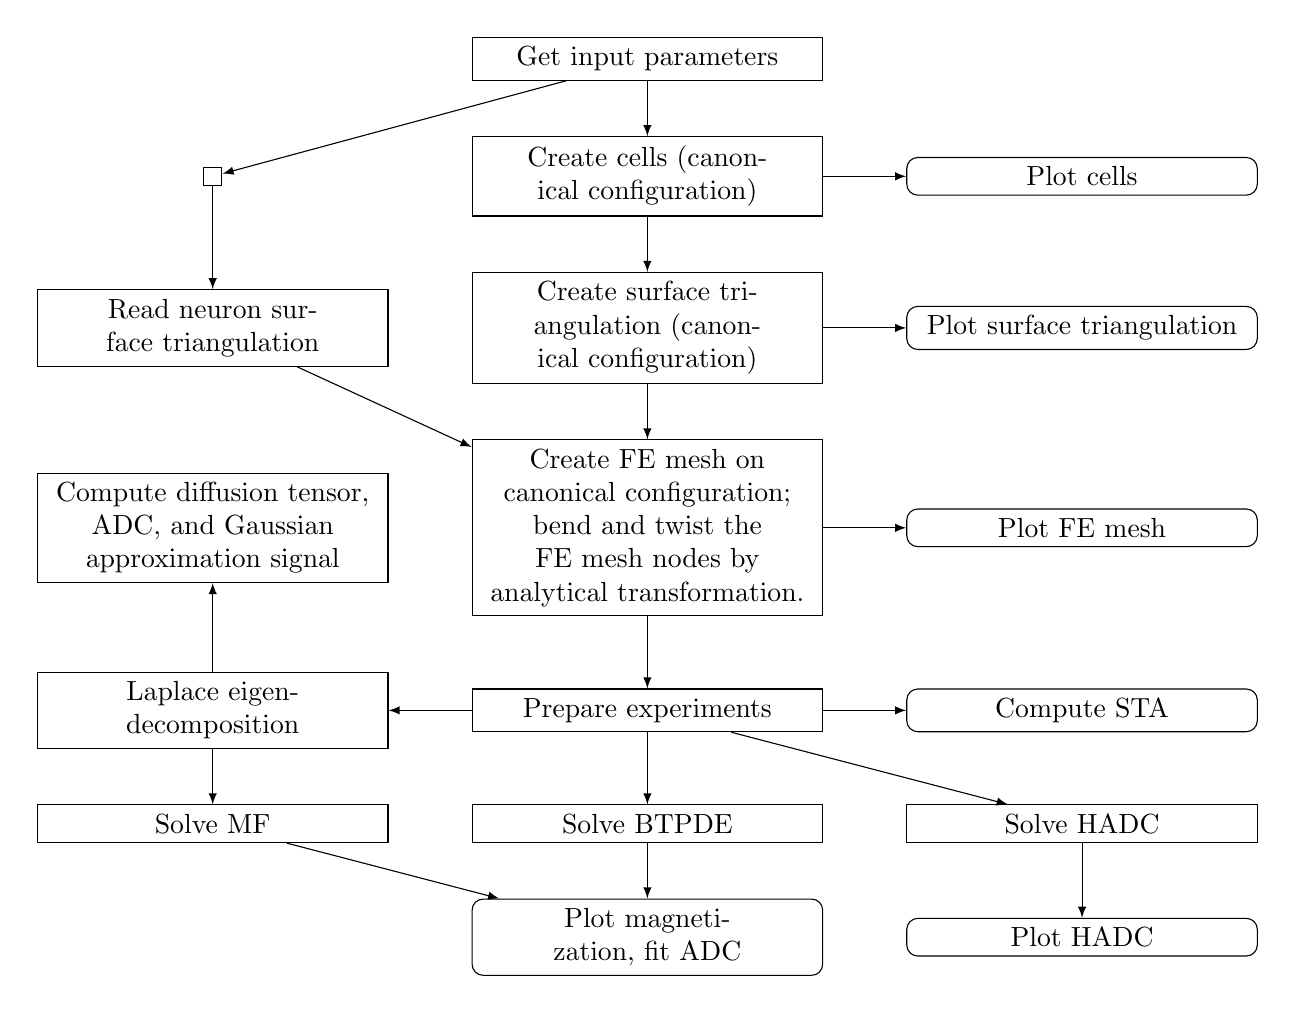
\begin{tikzpicture}
  \matrix (m)[matrix of nodes, column sep=3em, row sep=2em, align=center, nodes={rectangle,draw,anchor=center}]{
  & |[block]|{Get input parameters} & \\
  |[connector]| & |[block]|{Create cells (canonical configuration)} & |[decision]|{Plot cells } \\
  |[block]|{Read neuron surface triangulation} & |[block]|{Create surface triangulation (canonical configuration)} &            |[decision]| {Plot surface triangulation} \\
  |[block]|{Compute diffusion tensor, ADC, and Gaussian approximation signal} & |[block]|{Create FE mesh on canonical configuration; \\bend and twist the FE mesh nodes by analytical transformation.}         &           |[decision]|{Plot FE mesh}                                   \\
  |[block]|{Laplace eigendecomposition} & |[block]| {Prepare experiments} & |[decision]|{Compute STA} \\
  |[block]|{Solve MF} & |[block]|{Solve BTPDE} & |[block]|{Solve HADC} \\
  & |[decision]|{Plot magnetization, fit ADC} & |[decision]|{Plot HADC} \\
  };
  \path [>=latex,->] (m-1-2) edge (m-2-1);
  \path [>=latex,->] (m-2-1) edge (m-3-1);
  \path [>=latex,->] (m-3-1) edge (m-4-2);
  \path [>=latex,->] (m-1-2) edge (m-2-2);
  \path [>=latex,->] (m-2-2) edge (m-3-2);
  \path [>=latex,->] (m-3-2) edge (m-4-2);
  \path [>=latex,->] (m-4-2) edge (m-5-2);
  \path [>=latex,->] (m-5-2) edge (m-6-2);
  \path [>=latex,->] (m-6-2) edge (m-7-2);
  \path [>=latex,->] (m-2-2) edge (m-2-3);
  \path [>=latex,->] (m-3-2) edge (m-3-3);
  \path [>=latex,->] (m-4-2) edge (m-4-3);
  \path [>=latex,->] (m-5-2) edge (m-6-3);
  \path [>=latex,->] (m-5-2) edge (m-5-3);
  \path [>=latex,->] (m-6-3) edge (m-7-3);
  \path [>=latex,->] (m-5-2) edge (m-5-1);
  \path [>=latex,->] (m-5-1) edge (m-4-1);
  \path [>=latex,->] (m-5-1) edge (m-6-1);
  \path [>=latex,->] (m-6-1) edge (m-7-2);
\end{tikzpicture}

    \caption{Flow chart describing the work flow of SpinDoctor}
    \label{flowchart}
\end{figure}

The user also has to prepare the experiments. The function \verb+prepare_pde+ creates a compartment numbering system and assigns the material proper to the compartments. The function \verb+prepare_experiments+ checks the consistency of the experiments, and prepares some important quantities related to the gradient sequences (q-values, b-values, directions).

SpinDoctor provides different solvers, some of which only work under certain assumptions. The function \verb+solve_btpde+ computes the magnetization and signal at a precision only limited by the mesh refinement and ODE-solver tolerances. The ADC may be fitted from the resulting signal. The function \verb+solve_mf+ produces the same result as \verb+solve_btpde+, but at a much lower computational cost. This requires having previously computed the Laplace eigenvalues and eigenfunctions, from which a diffusion tensor and Gaussian approximation of the signal may be computed. The functions \verb+solve_hadc+ computes the ADC using a homogenized model, that assumes negligible permeability between compartments.


\subsection{User provided input parameters}

SpinDoctor expects the user to define a setup structure \verb+setup+ with different substructures. In the folder \verb+setups+, there are several example setups. Some important fields of \verb+setup+ are:
\begin{enumerate}
    \item \verb+name+ (string) file name for saving or loading geometry and results
    \item \verb+geometry+: structure containing geometry parameters. Format is given in Table \ref{table:setup_geometry}. If the cells are spheres or cylinders, the parameters for the geometrical configuration are provided in this structure.
    \item \verb+pde+: structure containing the PDE coefficients (material properties). Format is given in Table \ref{table:setup_pde}. This structure provides the material properties for each of the compartments \verb+in+, \verb+out+, \verb+ecs+, as well as their interfaces. If the \verb+in+ or \verb+ecs+ compartments are not included, the corresponding parameters are ignored.
    \item \verb+gradient+: structure defining the gradient sequences. Format is given in Table \ref{table:setup_gradient}. These gradients are parameterized by their amplitude, time profile (sequence), and direction.
\end{enumerate}

The sequences (time profiles) are instances of the MATLAB class \verb+Sequence+, which can be of type \verb+PGSE+, \verb+DoublePGSE+, \verb+CosOGSE+, \verb+SinOGSE+, or \verb+CustomSequence+. The latter requires providing a function handle representing the time profile. All the sequences can be called at time $t$ through the \verb+call+ method, whose integrals and b-values are obtained by the \verb+integral+ and \verb+bvalue_no_q+ methods. \verb+echotime+ provides the echo time $T_\text{echo}$ of the sequence. Each sequence comes with utility functions for string representation and information about their characteristic intervals. By default, a \verb+Sequence+ only requires a \verb+call+ method, while the other quantities can be computed numerically. However, for specific sequences, analytical expressions may be provided for the integral quantities.

In addition, the following possible substructures of \verb+setup+ defines the experiments to be carried out. Their precense triggers the corresponding experiment. They can be found in Table \ref{table:setup_experiments}:
\begin{itemize}
    \item \verb+btpde+ Solve BTPDE using P1 finite elements and built-in MATLAB ODE solvers. More details can be found in section \ref{sec:solve_btpde}.
    \item \verb+hadc+ Solve HADC using P1 finite elements and built-in MATLAB ODE solvers. More details can be found in section \ref{sec:solve_hadc}.
    \item \verb+mf+ Solve for the matrix formalism magnetization, given a P1-discretized Laplace eigendecomposition. More details can be found in section \ref{sec:solve_mf}.
    \item \verb+analytical+ Compute signal from analytical expressions for one multilayered cylinder or sphere. More details can be found in section \ref{sec:solve_analytical}.
    \item \verb+karger+ Solve FPK model.
\end{itemize}

\begin{table}
    \centering
    \begin{tabular}{|l|l|p{8cm}|} \hline

    Field name              & Example                 & Explanation                                                                                                                                                                            \\ \hline

    \verb+cell_shape+  & \verb+"cylinder"+  & \verb+"sphere"+, \verb+"cylinder"+ or \verb+"neuron"+                                                                                                               \\ \hline
    \verb+ncell+  & \verb+10+  & Number of cells (1 for neurons)                                                                                                                                                        \\ \hline
    \verb+rmin+  & \verb+1.5+  & Minimum cell radius                                                                                                                                                                    \\ \hline
    \verb+rmax+ & \verb+2.5+ & Maximum cell radius                                                                                                                                                                    \\ \hline
    \verb+dmin+ & \verb+1.5+ & Minimum (\%) distance between cells $\frac{d_\text{min}(r_\text{min}+r_\text{max})}{2}$                                                                                                \\ \hline
    \verb+dmax+ & \verb+2.5+ & Maximum (\%) distance between cells $\frac{d_\text{max}(r_\text{min}+r_\text{max})}{2}$                                                                                                \\ \hline
    \verb+height+ & \verb+20+ & Cylinder height (ignored if not cylinder)                                                                                                                                              \\ \hline
    \verb+deformation+ & \verb+[0.05 0.05]+ & [$\alpha$\quad $\beta$]; \newline $\alpha$ defines the amount of bend; \newline $\beta$ defines the amount of twist (in radians)                                                       \\ \hline
    \verb+include_in+ & \verb+true+ & Indicator for including in-compartment                                                                                                                                                 \\ \hline
    \verb+in_ratio+ & \verb+0.6+ & $\frac{r_\text{in}}{r_\text{out}} \in ]0,1[$                                                                                                                                           \\ \hline
    \verb+ecs_shape+ & \verb+"no_ecs"+ & Do not include ECS: \verb+"no_ecs"+;\newline Box wrap ECS: \verb+"box"+;\newline Convex hull: \verb+"convex_hull"+ \newline Tight wrap: \verb+"tight_wrap"+; \\ \hline
    \verb+ecs_ratio+ & \verb+0.3+ & ECS thickness as percentage of mean radius                                                                                                                                             \\ \hline
    \verb+refinement+ & \verb+0.5+ & Requested TetGen maximum tetrahedron volume (comment line to use default)                                                                                                              \\ \hline
\end{tabular}

    \caption{Structure containing geometry parameters.}
    \label{table:setup_geometry}
\end{table}

\begin{table}
    \centering
    \begin{tabular}{|l|l|p{8cm}|} \hline
    Field name              & Example                 & Explanation                                                               \\ \hline

    \verb+initial_density_in+  & \verb+1+  & \multirow{3}{*}{Initial spin density $\rho$}                              \\ \cline{1-2}
    \verb+initial_density_out+  & \verb+1+  &                                                                           \\ \cline{1-2}
    \verb+initial_density_ecs+  & \verb+1+  &                                                                           \\ \hline

    \verb+diffusivity_in+  & \verb+0.002+  & \multirow{3}{*}{Diffusion coefficient $\sigma$. Can also be a 3x3-tensor} \\ \cline{1-2}
    \verb+diffusivity_out+  & \verb+0.002+ &                                                                           \\ \cline{1-2}
    \verb+diffusivity_ecs+ & \verb+0.002+ &                                                                           \\ \hline

    \verb+relaxation_in+ & \verb+Inf+ & \multirow{3}{*}{$T_2$-relaxation times (for no relaxation: Inf)}          \\ \cline{1-2}
    \verb+relaxation_out+ & \verb+5000+ &                                                                           \\ \cline{1-2}
    \verb+relaxation_ecs+ & \verb+5000+ &                                                                           \\ \hline

    \verb+permeability_in_out+ & \verb+1e-3+ & \multirow{5}{*}{Permeability coefficient $\kappa$}                        \\ \cline{1-2}
    \verb+permeability_out_ecs+ & \verb+1e-4+ &                                                                           \\ \cline{1-2}
    \verb+permeability_in+ & \verb+0+ &                                                                           \\ \cline{1-2}
    \verb+permeability_out+ & \verb+0+ &                                                                           \\ \cline{1-2}
    \verb+permeability_ecs+ & \verb+0+ &                                                                           \\ \hline
\end{tabular}

    \caption{Structure containing PDE parameters.}
    \label{table:setup_pde}
\end{table}

\begin{table}
    \begin{tabular}{|l|l|p{6cm}|} \hline

    Field name              & Example                 & Explanation                                                                                                                                                               \\ \hline

    \verb+values+  & \verb+[10 100 400 1000]+  & $\|\vec{g}\|$-values, q-values or b-values to consider                                                                                                                    \\ \hline
    \verb+values_type+  & \verb+"b"+  & \verb+"g"+, \verb+"q"+ or \verb+"b"+                                                                                                  \\ \hline
    \verb+sequences+  & \verb+{PGSE(100, 5000)}+  & Gradient sequences; \verb+PGSE(delta, Delta)+, \verb+DoublePGSE(delta, Delta, tpause)+, \verb+CosOGSE(delta, Delta, nperiod)+, \verb+SinOGSE(delta, Delta, nperiod)+ or \verb+CustomSequence(delta, Delta,+ \verb+@timeprofile)+ \\ \hline
    \verb+directions+ & \verb+[1.0; 0.0; 0.0]+ & Gradient directions of size \verb+[3 x ndirection]+ (no need to normalize)                                                                                                \\ \hline
\end{tabular}

    \caption{Structure defining gradient sequences.}
    \label{table:setup_gradient}
\end{table}

\begin{table}
    \begin{tabular}{|l|l|p{6cm}|} \hline

    Field name              & Example                 & Explanation                                                                                                  \\ \hline

    \verb+btpde+  & \verb+struct+  & Substructure for solving the BTPDE (comment out to skip)                                                     \\ \hline
    \verb+btpde.ode_solver+  & \verb+@ode15s+  & Function handle for ODE solver (comment to use default)                                                      \\ \hline
    \verb+btpde.reltol+  & \verb+1e-4+  & Relative tolerance for ODE solver                                                                            \\ \hline
    \verb+btpde.abstol+  & \verb+1e-6+  & Absolute tolerance for ODE solver                                                                            \\ \hline

    \verb+btpde_midpoint+  & \verb+struct+ & Substructure for solving the BTPDE using Crank-Nicolson solver (comment out to skip)                         \\ \hline
    \verb+btpde_midpoint.implicitness+ & \verb+0.5+ & Implicitness parameter $\theta$: 0.5 for Crank-Nicolson (second order), 1.0 for Implicit Euler (first order) \\ \hline
    \verb+btpde_midpoint.timestep+ & \verb+5.0+ & Uniform time step $\mathrm{d} t$                                                                             \\ \hline

    \verb+hadc+ & \verb+struct+ & Substructure for solving the HADC model (comment out to skip)                                                \\ \hline
    \verb+hadc.ode_solver+ & \verb+@ode15s+ & Function handle for ODE solver (comment to use default)                                                      \\ \hline
    \verb+hadc.reltol+ & \verb+1e-4+ & Relative tolerance for ODE solver                                                                            \\ \hline
    \verb+hadc.abstol+ & \verb+1e-4+ & Absolute tolerance for ODE solver                                                                            \\ \hline

    \verb+mf+ & \verb+struct+ & Substructure for solving for the Matrix Formalism (comment out to skip)                                      \\ \hline
    \verb+mf.length_scale+ & \verb+3+ & Minimum length scale of Laplace eigenfunctions                                                               \\ \hline
    \verb+mf.neig_max+ & \verb+100+ & Maximum number of eigenvalues. To compute all: \verb+Inf+                                       \\ \hline
    \verb+mf.ninterval+ & \verb+50+ & Number of intervals to discretize time profile (if not PGSE)                                                 \\ \hline

    \verb+analytical+ & \verb+struct+ & Substructure for solving for the analytical model (comment out to skip)                                      \\ \hline
    \verb+analytical.length_scale+ & \verb+3+ & Minimum length scale of radial Laplace eigenfunctions                                                        \\ \hline
    \verb+analytical.eigstep+ & \verb+1e-6+ & Minimium distance between two radial eigenvalues                                                             \\ \hline

    \verb+karger+ & \verb+struct+ & Substructure for solving for the FPK model (comment out to skip)                                             \\ \hline
    \verb+karger.ndirection+ & 50                      & Number of direction to compute effective diffusion tensor                                                    \\ \hline
    \verb+karger.ode_solver+ & \verb+@ode23t+ & Function handle for ODE solver (comment to use default)                                                      \\ \hline
    \verb+karger.reltol+ & \verb+1e-4+ & Relative tolerance for ODE solver                                                                            \\ \hline
    \verb+karger.abstol+ & \verb+1e-6+ & Absolute tolerance for ODE solver                                                                            \\ \hline
\end{tabular}

    \caption{Structures containing simulation experiment parameters.}
    \label{table:setup_experiments}
\end{table}


\subsection{Important output quantities}

In Table \ref{table:outputs} we list some useful quantities that are the outputs of SpinDoctor. The braces in the ``Size'' column denote MATLAB cell array structures and the brackets denote MATLAB matrix data structures.

\begin{table}
    \centering
    \begin{tabular}{|l|l|p{5cm}|} \hline
    Variable name          & Size                                                       & Explanation                                                                         \\ \hline
    \verb+magnetization+ & \{ncmpt $\times$ namp $\times$ nseq $\times$ ndir\}[nnode] & Solution of the BTPDE for each compartment                                          \\ \hline
    \verb+signal+ & [ncmpt $\times$ namp $\times$ nseq $\times$ ndir]          & Signal (integral of magnetization) at $T_\text{echo}$ in each compartment.          \\ \hline
    \verb+signal_allcmpts+ & [namp $\times$ nseq $\times$ ndir]                         & Signal (integral of magnetization) at $T_\text{echo}$ summed over all compartments. \\ \hline
    \verb+adc+ & [ncmpt $\times$ nseq $\times$ ndir]                        & ADC in each compartment.                                                            \\ \hline
    \verb+adc_allcmpts+ & [nseq $\times$ ndir]                                       & ADC accounting for all compartments.                                                \\ \hline
    \verb+lap_eig.values+ & [neig $\times$ 1]                                          & Laplace eigenvalues                                                                 \\ \hline
    \verb+lap_eig.funcs+ & [nnode $\times$ neig]                                      & Laplace eigenfunctions                                                              \\ \hline
    \verb+lap_eig.moments+ & [neig $\times$ neig $\times$ 3]                            & First order moments of the product pairs of Laplace eigenfunctions                  \\ \hline
    \verb+diffusion_tensor+ & [3 $\times$ 3 $\times$ nseq]                               & Effective diffusion tensors                                                         \\ \hline
\end{tabular}

    \caption{Some important SpinDoctor output quantities.}
    \label{table:outputs}
\end{table}

% \begin{table}
%   \centering
%   \begin{tabular}{|l|l|p{5.4cm}|}
    \hline
    Variable name                 & Size                                                          & Explanation                                                        \\ \hline
    \verb+lap_eig+.values & [neig $\times$ 1]                                             & Laplace eigenvalues                                                \\ \hline
    \verb+lap_eig.funcs+        & [nnode $\times$ neig]                                         & Laplace eigenfunctions                                             \\ \hline
    \verb+lap_eig.moments+        & [neig $\times$ neig $\times$ 3]                               & First order moments of the product pairs of Laplace eigenfunctions \\ \hline
    \verb+diffusion_tensor+        & [3 $\times$ 3 $\times$ nseq]                                  & Effective diffusion tensors                                        \\ \hline
    \verb+mf.magnetization+        & \{ncmpt$\times$namp$\times$nseq$\times$ndir\}[nnode$\times$1] & Resulting magnetization fields                                     \\ \hline
    \verb+mf.signal+        & [ncmpt $\times$ namp $\times$ nseq $\times$ ndir]             & MF signal in the compartments                                      \\ \hline
    \verb+mf.signal_allcmpts+        & [namp $\times$ nseq $\times$ ndir]                            & MF signal summed over all compartments                             \\ \hline
    \verb+mfga.signal+        & [ncmpt $\times$ namp $\times$ nseq $\times$ ndir]             & MFGA signal in the compartments.                                   \\ \hline
    \verb+mfga.signal_allcmpts+        & [namp $\times$ nseq $\times$ ndir]                            & MFGA signal summed over all compartments                           \\ \hline
\end{tabular}

%   \caption{Some important Matrix Formalism Module output quantities.}
%   \label{table:outputs_mf}
% \end{table}


\subsection{Important functions}

In Table \ref{table:functions_spindoctor} we list some important functions of SpinDoctor. For detailed information about them, including argument lists, please read the online documentation.

\begin{table}
    \centering
    \begin{tabular}{|l|p{10cm}|} \hline
    Function name           & Purpose                                                                                                                                                                                                     \\ \hline
    \verb+prepare_experiments+  & Prepare magnetic gradient sequences, directions, and BTPDE, HADC and MF experiments                                                                                                                         \\ \hline
    \verb+prepare_pde+  & Set up the PDE model in the geometrical compartments                                                                                                                                                        \\ \hline
    % \verb+create_cells+ & Create the geometrical configuration. \\ \hline
    \verb+create_geometry+  & Create or load cells, surface geometry and finite element mesh                                                                                                                                              \\ \hline
    % \verb+read_tetgen+ & Read the finite elements mesh \\ \hline
    % \verb+get_volume_sa+ & Get the volume and the surface area quantities from the finite elements mesh. \\ \hline
    % \verb+create_directions+ & Provide gradient directions uniformly distributed in unit 3D sphere or 2D circle. \\ \hline
    \verb+solve_btpde+  & Compute the BTPDE magnetization and signal                                                                                                                                                                  \\ \hline
    \verb+solve_hadc+  & Compute the ADC from the HADC model                                                                                                                                                                         \\ \hline
    \verb+fit_signal+ & Fit the ADC and signal for zero b-weighting from the BTPDE signal.                                                                                                                                          \\ \hline
    \verb+compute_adc_sta+ & Compute the short time approximation in one diffusion-encoding direction.                                                                                                                                   \\ \hline
    \verb+compute_free_diffusion+ & Compute the free diffusion ADC and signal.                                                                                                                                                                  \\ \hline
    \verb+plot_cells+ &                                                                                                                                                                                                             \\ \hline
    \verb+plot_surface_triangulation+ &                                                                                                                                                                                                             \\ \hline
    \verb+plot_femesh+ & Display the finite elements mesh.                                                                                                                                                                           \\ \hline
    \verb+plot_geometry_info+ &                                                                                                                                                                                                             \\ \hline
    \verb+plot_signal+ & Display the simulated signal in one diffusion-encoding direction.                                                                                                                                           \\ \hline
    \verb+plot_timing+ &                                                                                                                                                                                                             \\ \hline
    \verb+plot_adc+ & Display the simulated ADC in one diffusion-encoding direction.                                                                                                                                              \\ \hline
    \verb+plot_field+ & Display the PDE solution on the finite elements mesh. If the finite elements mesh is too large, the magnetization should not be outputted from the solution of the BTPDE, and this function cannot be used. \\ \hline
    \verb+plot_hardi+ & Display simulation results in multiple diffusion-encoding directions.                                                                                                                                       \\ \hline
\end{tabular}

    \caption{Some important functions in SpinDoctor.}
    \label{table:functions_spindoctor}
\end{table}


In Table \ref{table:functions_mf} we list important functions of the Matrix Formalism Module. For detailed information about them, including argument lists, please read the online documentation.

\begin{table}
    \centering
    \begin{tabular}{|l|p{10cm}|} \hline
    Function name                                  & Purpose                                                                                                            \\ \hline
    \verb+compute_laplace_eig+                         & Compute the Laplace eigenvalues, eigenfunctions and the first order moments of the products of the eigenfunctions. \\ \hline
    % \verb+compute_laplace_eig_subinterval+ & Compute the Laplace eigenvalues, eigenfunctions and the first order moments of the products of the eigenfunctions on different intervals separately (requires PDE Toolbox) \\ \hline
    \verb+eig2length+, \verb+length2eig+ & Convert the computed eigenvalues into a length scale, and vice-versa                                               \\ \hline
    \verb+mf_jn+                         & Compute the quantity $J(\lambda_n,f)$                                                                              \\ \hline
    \verb+compute_mf_diffusion_tensor+                         & Computes the effective diffusion tensor                                                                            \\ \hline
    \verb+plot_diffusion_tensor+                         & Display the effective diffusion tensor                                                                             \\ \hline
    \verb+solve_mf+                         & Compute the Matrix Formalism magnetization and signal                                                              \\ \hline
    \verb+compute_mf_signal+                         & Compute the Matrix Formalism total signal only                                                                     \\ \hline
    \verb+compute_mfga_signal+                        & Computes the Matrix Formalism Gaussian Approximation total signal                                                  \\ \hline
\end{tabular}

    \caption{Some important functions in the Matrix Formalism Module.}
    \label{table:functions_mf}
\end{table}



\subsection{Create cells (canonical configuration)}

SpinDoctor supports the placement of a group of non-overlapping cells in close vicinity to each other. There are two proposed configurations, one composed of spheres, the other composed of cylinders. The algorithm is described in Algorithm \ref{algo:create_cells}.

\begin{algorithm}
    Generate a large number of possible cell centers.

Compute the \soutnew{}{minimum} distance, $d$, between the current center and previously accepted cells.

Find the intersection of [$d-d_\text{max} r_\text{mean}$, $d-d_\text{min} r_\text{mean}$] and $[r_\text{min}, r_\text{max}]$, where $r_\text{mean}=\frac{r_\text{min}+r_\text{max}}{2}$. If the intersection is not empty, then take the middle of the intersection as the new radius and accept the new center. Otherwise, reject the center.

Loop through the possible centers until get $N_\text{cell}$ accepted cells.

    \caption{Placing $N_\text{cell}$ non-overlapping cells.}
    \label{algo:create_cells}
\end{algorithm}

SpinDoctor provides a routine to plot the cells to see if the configuration is acceptable (see Fig. \ref{fig:plot_cells}).
\begin{figure}
    \centering
    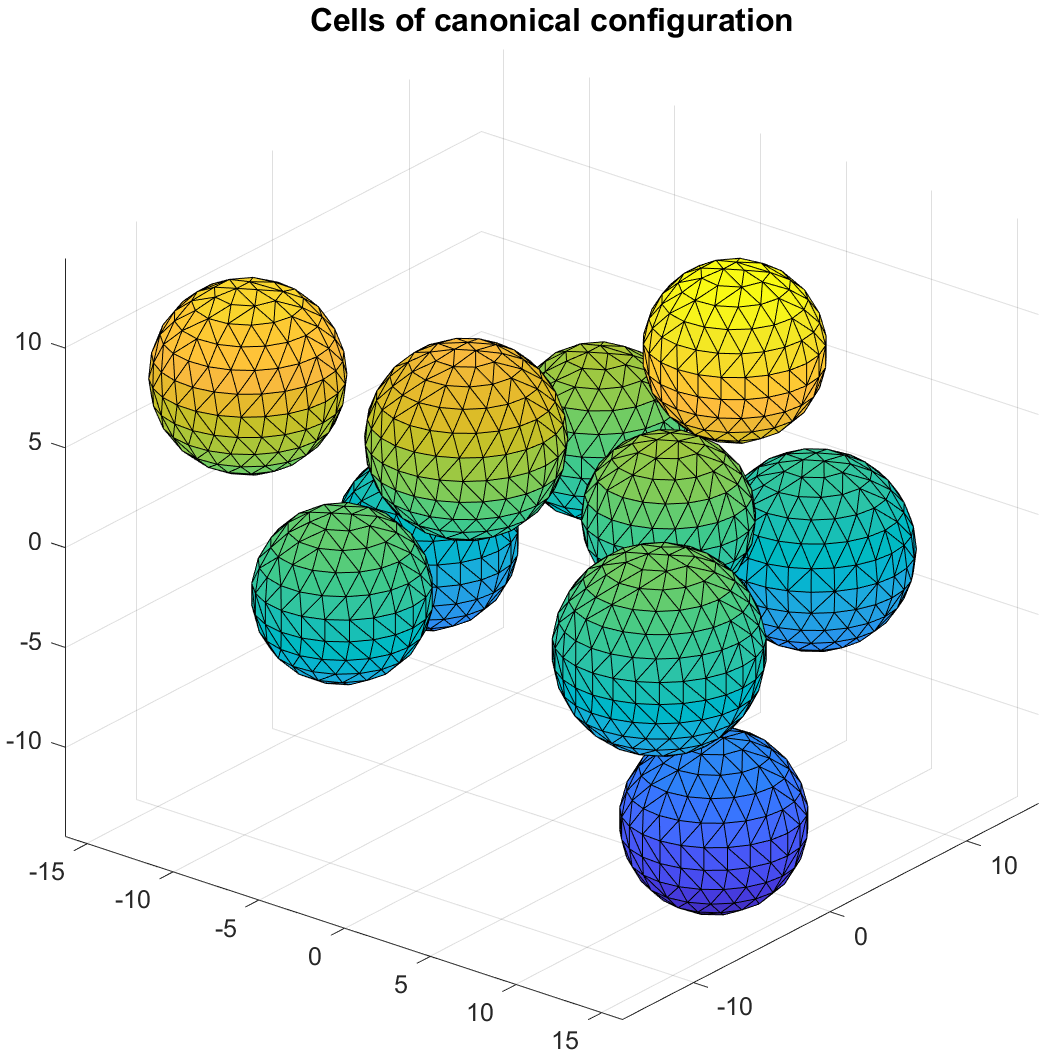
\includegraphics[width=0.49\textwidth]{plot_cells/spheres.png}
    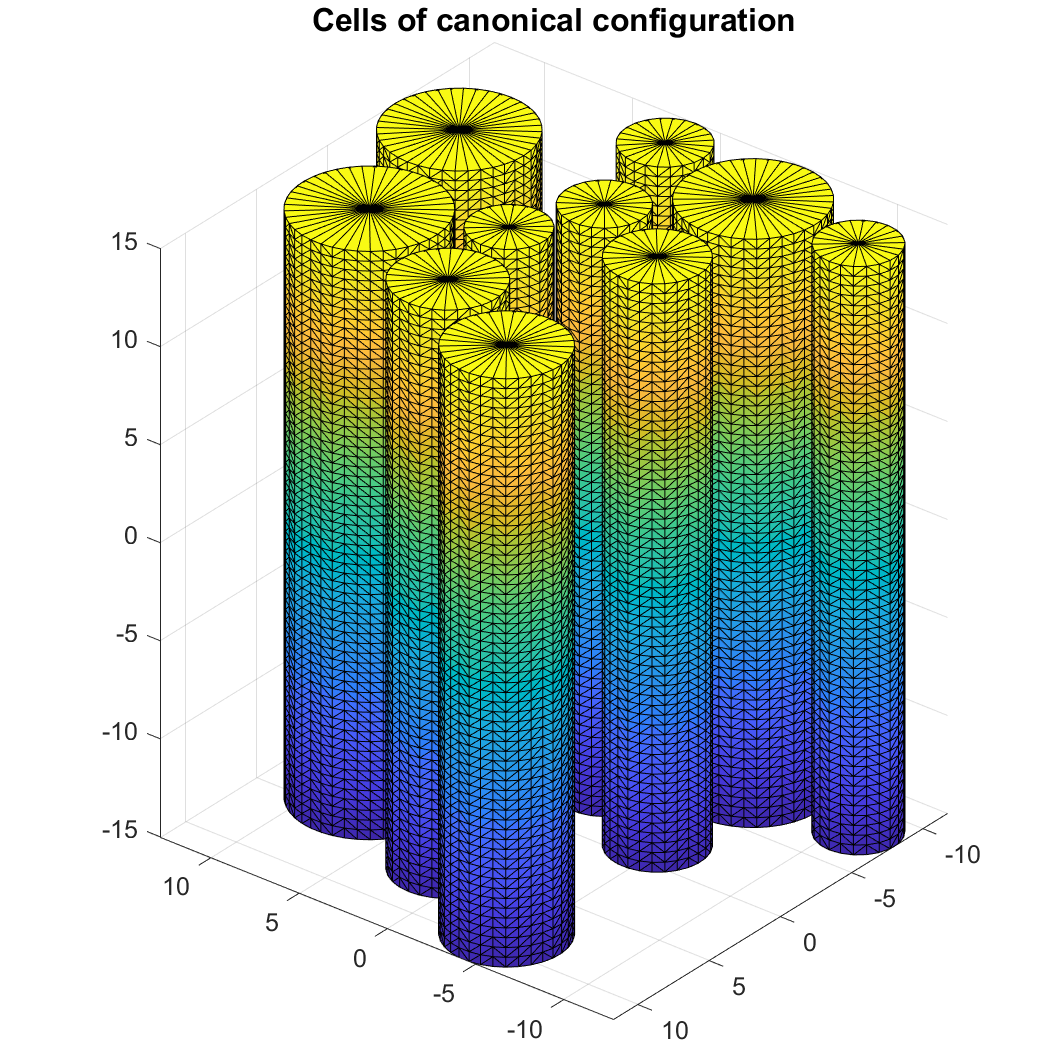
\includegraphics[width=0.49\textwidth]{plot_cells/cylinders.png}
    \caption{SpinDoctor plots cells in the canonical configuration.}
    \label{fig:plot_cells}
\end{figure}



\subsection{Create surface triangulation}

Finite element mesh generation software requires a good surface triangulation. This means the surface triangulation needs to be water-tight and does not self-intersect. How closely these requirements are met in floating point arithmetic has a direct impact on the quality of the finite element mesh generated.

It is often difficult to produce a good surface triangulation for arbitrary geometries. Thus, we restrict the allowed shapes to cylinders and spheres. Below in Algorithms \ref{algo:surface_triangulation_spheres} and \ref{algo:surface_triangulation_cylinders} we describe how to obtain a surface triangulation for spherical cells with nucleus, cylindrical cells with myelin layer, and the ECS (box or tightly wrapped). We describe a canonical configuration where the cylinders are placed parallel to the $z$-axis. More general shapes are obtained from the canonical configuration by coordinate transformation in a later step.

\begin{algorithm}
    Suppose we have $N_\text{cell}$ spherical cells with nucleus. Denote a sphere with center $c$ and radius $R$ by $S(c, R)$, we use the built-in functions (convex hull, delaunay triangulation) in MATLAB to get its surface triangulation, $T(c, R)$. Call the radii of the nucleus $r_1, \dots, r_{N_\text{cell}}$ and the radii of the cells $R_1, \dots, R_{N_\text{cell}}$. Then the boundaries between the cytoplasm and the nucleus are
$$\{\Gamma_i = T(c_i, r_i)\}, \quad i = 1, \dots, N_\text{cell};$$
and between the cytoplasm and the ECS
$$\{\Sigma_i = T(c_i, R_i)\}, \quad i = 1, \dots, N_\text{cell};$$
For the box ECS, we find the coordinate limits of the set
$$\bigcup_{i=1}^{N_\text{cell}} S(c_i,R_i) \subset [x_0,x_f]\times [y_0,y_f] \times [z_0,z_f]$$
and add a gap $k = \text{ecs\_gap}\times \max\{x_f-x_0,y_f-y_0,z_f-z_0\}$ to make a box
$$B = [x_0 - k, x_f + k]\times [y_0 - k, y_f + k] \times [z_0 - k, z_f + k].$$
We put 2 triangles on each face of $B$ to make a surface triangulation $\Psi$ with 12 triangles.

For the tight-wrap ECS, we increase the cell radius by a gap size and take the union
$$W = \bigcup_{i=1}^{N_\text{cell}} S(c_i,R_i+\text{ecs\_gap}\times R_\text{mean}),$$
where $R_\text{mean}=\frac{R_\text{min}+R_\text{max}}{2}$. We use the alphaShape function in MATLAB to find a surface triangulation $\Psi$ that contains $W$.

    \caption{Surface triangulation of spherical cells and ECS.}
    \label{algo:surface_triangulation_spheres}
\end{algorithm}

\begin{algorithm}
    Suppose we have $N_\text{cell}$ cylindrical cells with a myelin layer, all with height $H$. Denote a disk with center $c$ and radius $R$ by $D(c, R)$, and the circle with the same center and radius by $C(c, R)$. Let the radii of the axons be $r_1, \dots, r_{N_\text{cell}}$ and the radii of the cells be $R_1, \dots, R_{N_\text{cell}}$, meaning the thickness of the myelin layer is $R_i - r_i$.

The boundary between the axon and the myelin layer is:
$$C(c_i,r_i)\times [-H/2,H/2]$$
We discretize $C(c_i,r_i)$ as a polygon $P(c_i,r_i)$ and place one at $z = -H/2$ and one at $z = H/2$. Then we connect the corresponding vertices of $P(c_i,r_i)\times\{-H/2\}$ and $P(c_i,r_i)\times\{H/2\}$ and add a diagonal on each panel to get a surface triangulation $\Gamma_i$.

Between the myelin layer and the ECS we discretize $C(c_i,R_i)$ as a polygon and place one at $z=-H/2$ and one at $z = H/2$ to get a surface triangulation $\Sigma_i$.

For the box ECS, we find the coordinate limits of the union of $D(c_i,r_i)$ and add a gap to make a rectangle in two dimensions. Then we place the rectangle at $z=-H/2$ and at $z=H/2$ to get a box. Finally, the box is given a surface triangulation with 12 triangles.

For tight-wrap ECS, we increase the cell radius by a gap size and take the union
$$W = \bigcup_{i=1}^{N_\text{cell}} D(c_i, R_i + k R_\text{mean}).$$
We use the alphaShape function in MATLAB to find a two dimensional polygon $Q$ that contains $W$. We place $Q$ at $z=-H/2$ and at $z=H/2$ and connect corresponding vertices, adding a diagonal on each panel. Suppose $Q$ is a polygon with $n$ vertices, then the surface triangulation of the side of the ECS will have $2n$ triangles.

The above procedure produces a surface triangulation for the boundaries that are parallel to $z$-axis. We now must close the top and bottom. The top and bottom boundaries is just the interior of $Q$. However, the surface triangulation cannot be done on $Q$ directly. We must cut out $D(c_i,r_i)$, the disk which touches the axon, and $A_i = D(c_i,R_i)-D(c_i,r_i)$, the annulus which touches the myelin. Then we triangulate $Q-\bigcup_{i=1}^{N_\text{cell}} D(c_i,R_i)$ using the MATLAB built-in function that triangulates a polygon with holes to get the boundary that touches the ECS. The surface triangulation for $A_i$ and $D(c_i,r_i)$ is straightforward.

    \caption{Surface triangulation of cylindrical cells and ECS.}
    \label{algo:surface_triangulation_cylinders}
\end{algorithm}

SpinDoctor provides a routine to plot the surface triangulation (see Fig. \ref{fig:plot_surface_triangulation}).

\begin{figure}
    \centering
    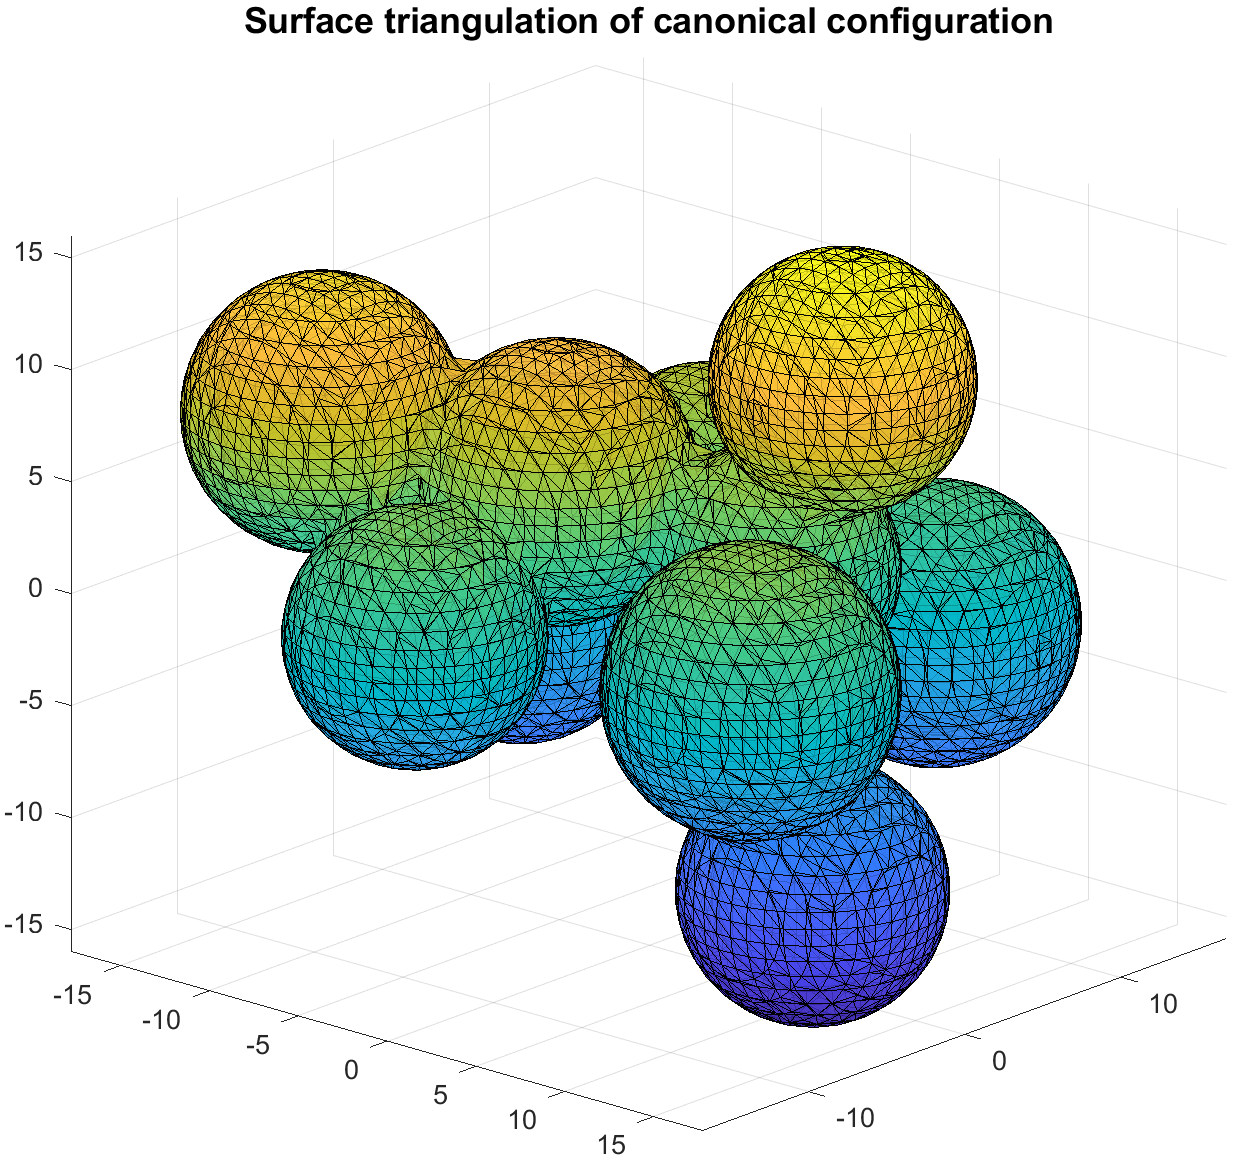
\includegraphics[width=0.49\textwidth]{plot_surftri/spheres.png}
    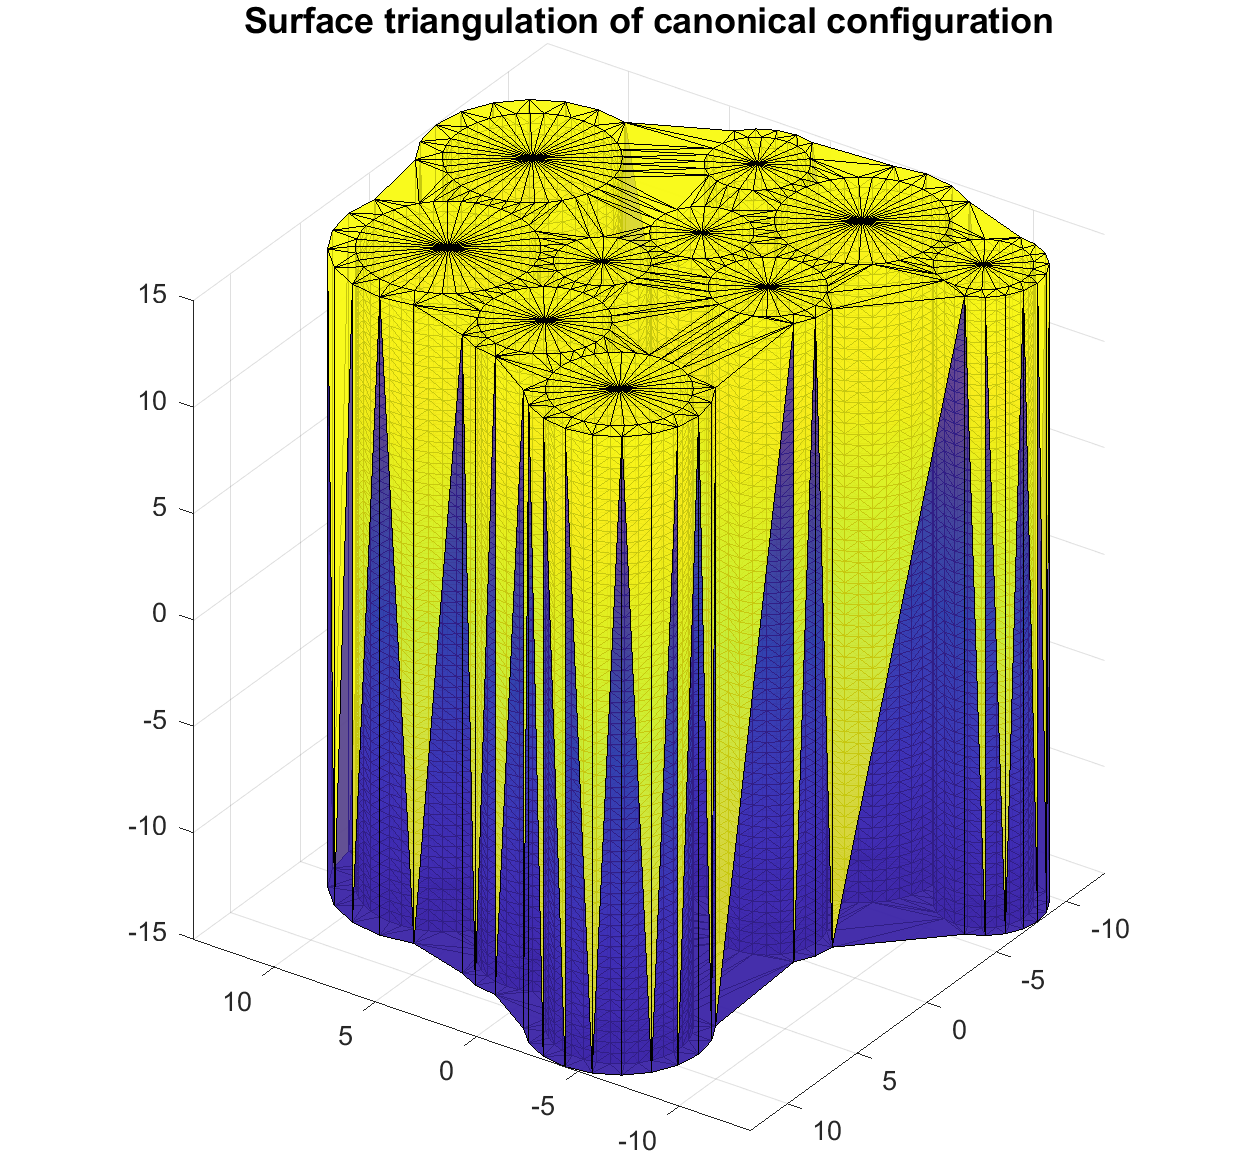
\includegraphics[width=0.49\textwidth]{plot_surftri/cylinders.png}
    \caption{SpinDoctor plots the surface triangulation of the canonical configuration. Left: spherical cells with ECS; Right: cylindrical cells with ECS.}
    \label{fig:plot_surface_triangulation}
\end{figure}




\subsection{Finite element mesh generation}

SpinDoctor calls Tetgen \cite{tetgen}, an external package (executable files are included in the toolbox package), to create a tetrahedra finite elements mesh from the surface triangulation generated by Algorithms \ref{algo:surface_triangulation_spheres} and \ref{algo:surface_triangulation_cylinders}. The FE mesh is generated on the canonical configuration. The numbering of the compartments and boundaries used by SpinDoctor are given in Tables \ref{table:cmpts_labels} and \ref{table:bdys_labels}. The labels are related to the values of the intrinsic diffusion coefficient, the initial spin density, and the permeability requested by the user. Then the FE mesh nodes are deformed analytically by a coordinate transformation, described in Algorithm \ref{algo:bend_twist}.
\begin{table}
    \centering
    \begin{tabular}{|c|c|c|c|}

	\multicolumn{4}{c}{Spherical cells without nucleus}                                                          \\ \hline
	Cmpt   &                             & Nucleus                                       & ECS                   \\ \hline
	Label  &                             & out                                           & ecs                   \\ \hline
	Number &                             & $[1, \dots, n_\text{cell}]$                   & $n_\text{cell} + 1$   \\ \hline

	\multicolumn{4}{c}{Spherical cells with nucleus}                                                             \\ \hline
	Cmpt   & Nucleus                     & Cytoplasm                                     & ECS                   \\ \hline
	Label  & in                          & out                                           & ecs                   \\ \hline
	Number & $[1, \dots, n_\text{cell}]$ & $[n_\text{cell} + 1, \dots, 2 n_\text{cell}]$ & $2 n_\text{cell} + 1$ \\ \hline

	\multicolumn{4}{c}{Cylindrical cells without myelin}                                                         \\ \hline
	Cmpt   &                             & Axon                                          & ECS                   \\ \hline
	Label  &                             & out                                           & ecs                   \\ \hline
	Number &                             & $[1, \dots, n_\text{cell}]$                   & $n_\text{cell} + 1$   \\ \hline

	\multicolumn{4}{c}{Cylindrical cells with myelin}                                                            \\ \hline
	Cmpt   & Axon                        & Myelin                                        & ECS                   \\ \hline
	Label  & in                          & out                                           & ecs                   \\ \hline
	Number & $[1, \dots, n_\text{cell}]$ & $[n_\text{cell} + 1, \dots, 2 n_\text{cell}]$ & $2 n_\text{cell}+1$   \\ \hline

	\multicolumn{4}{c}{Neuron}                                                                                   \\ \hline
	Cmpt   &                             & Neuron                                        & ECS                   \\ \hline
	Label  &                             & out                                           & ecs                   \\ \hline
	Number &                             & 1                                             & 2                     \\ \hline
\end{tabular}

    \caption{The labels and numbers of compartments.}
    \label{table:cmpts_labels}
\end{table}

\begin{table}
    \centering
    \begin{tabular}{|c|c|c|c|c|c|}

    \multicolumn{6}{c}{Spherical cells without nucleus}                                                                                                                                                                               \\ \hline
    Label                     &                             & out,ecs                                       &                                                &                                                & ecs                   \\ \hline
    Number                    &                             & $[1,\dots,n_\text{cell}]$                     &                                                &                                                & $n_\text{cell}+1$     \\ \hline

    \multicolumn{6}{c}{Spherical cells with nucleus}                                                                                                                                                                                  \\ \hline
    Label                     & in,out                      & out,ecs                                       &                                                &                                                & ecs                   \\ \hline
    Number                    & $[1,\dots,n_\text{cell}]$   & $[n_\text{cell}+1,\dots,2n_\text{cell}]$      &                                                &                                                & $2n_\text{cell}+1$    \\ \hline

    \multicolumn{6}{c}{Cylindrical cells without myelin}                                                                                                                                                                              \\ \hline
    \multirow{2}{*}{Boundary} &                             & Cylinder                                      &                                                & Cylinder                                       & Outer ECS             \\
                              &                             & side wall                                     &                                                & top and bottom                                 & boundary              \\ \hline
    Label                     &                             & out,ecs                                       &                                                & out                                            & ecs                   \\ \hline
    Number                    &                             & $[1, \dots, n_\text{cell}]$                   &                                                & $[n_\text{cell} + 1, \dots, 2 n_\text{cell}]$  & $2n_\text{cell}+1$    \\ \hline

    \multicolumn{6}{c}{Cylindrical cells with myelin}                                                                                                                                                                                 \\ \hline
    \multirow{2}{*}{Boundary} & Inner cylinder              & Outer cylinder                                & Inner cylinder                                 & Outer cylinder                                 & Outer ECS             \\
                              & side wall                   & side wall                                     & top and bottom                                 & top and bottom                                 & boundary              \\ \hline
    Label                     & in,out                      & out,ecs                                       & in                                             & out                                            & ecs                   \\ \hline
    Number                    & $[1, \dots, n_\text{cell}]$ & $[n_\text{cell} + 1, \dots, 2 n_\text{cell}]$ & $[2n_\text{cell} + 1, \dots, 3 n_\text{cell}]$ & $[3n_\text{cell} + 1, \dots, 4 n_\text{cell}]$ & $4 n_\text{cell} + 1$ \\ \hline

    \multicolumn{6}{c}{Neuron}                                                                                                                                                                                                        \\ \hline
    Boundary                  &                             &                                               &                                                & Neuron                                         &                       \\ \hline
    Label                     &                             &                                               &                                                & out                                            &                       \\ \hline
    Number                    &                             &                                               &                                                & 1                                              &                       \\ \hline

    \multicolumn{6}{c}{Neuron with ECS}                                                                                                                                                                                               \\ \hline
    Boundary                  &                             & Neuron                                        &                                                &                                                & ECS                   \\ \hline
    Label                     &                             & out,ecs                                       &                                                &                                                & ecs                   \\ \hline
    Number                    &                             & 1                                             &                                                &                                                & 2                     \\ \hline
\end{tabular}

    \caption{The labels and numbers of boundaries.}
    \label{table:bdys_labels}
\end{table}

\begin{algorithm}
    The external package Tetgen \cite{tetgen} generates the finite element mesh that keeps track of the different compartments and the interfaces between them. The mesh is saved in several text files.

The connectivity matrices of the finite elements and facets are not modified by the coordinates transformation described below. The nodes are transformed by
bending and twisting as described next.

The set of FE mesh nodes $\{x_i,y_i,z_i\}$ are transformed in the following ways:

Twisting around the $z$-axis with a user-chosen twisting parameter $\alpha_\text{twist}$ is defined by
\ben
\begin{split}
  \vthree{x}{y}{z} & \rightarrow \begin{bmatrix}
    \cos(\alpha_\text{twist} z) & -\sin(\alpha_\text{twist} z) & 0 \\
    \sin(\alpha_\text{twist} z) & \cos(\alpha_\text{twist} z)  & 0 \\
    0                           & 0                            & 1
  \end{bmatrix} \vthree{x}{y}{z}.
\end{split}
\een

Bending on the $x-z$ plane with a user-chosen bending parameter $\alpha_\text{bend}$ is defined by
\ben
\vthree{x}{y}{z} \rightarrow
\vthree{x+
  \alpha_\text{bend}z^2}{y}{z}.
\een

Given $[\alpha_\text{bend},\alpha_\text{twist}]$, bending is performed after twisting.

    \caption{Bending and twisting of the FE mesh of the canonical configuration.}
    \label{algo:bend_twist}
\end{algorithm}

SpinDoctor provides a routine to plot the FE mesh (see Fig. \ref{fig:plot_fe_mesh} for cylinders and ECS that have been bent and twisted).

\begin{figure}
    \centering
    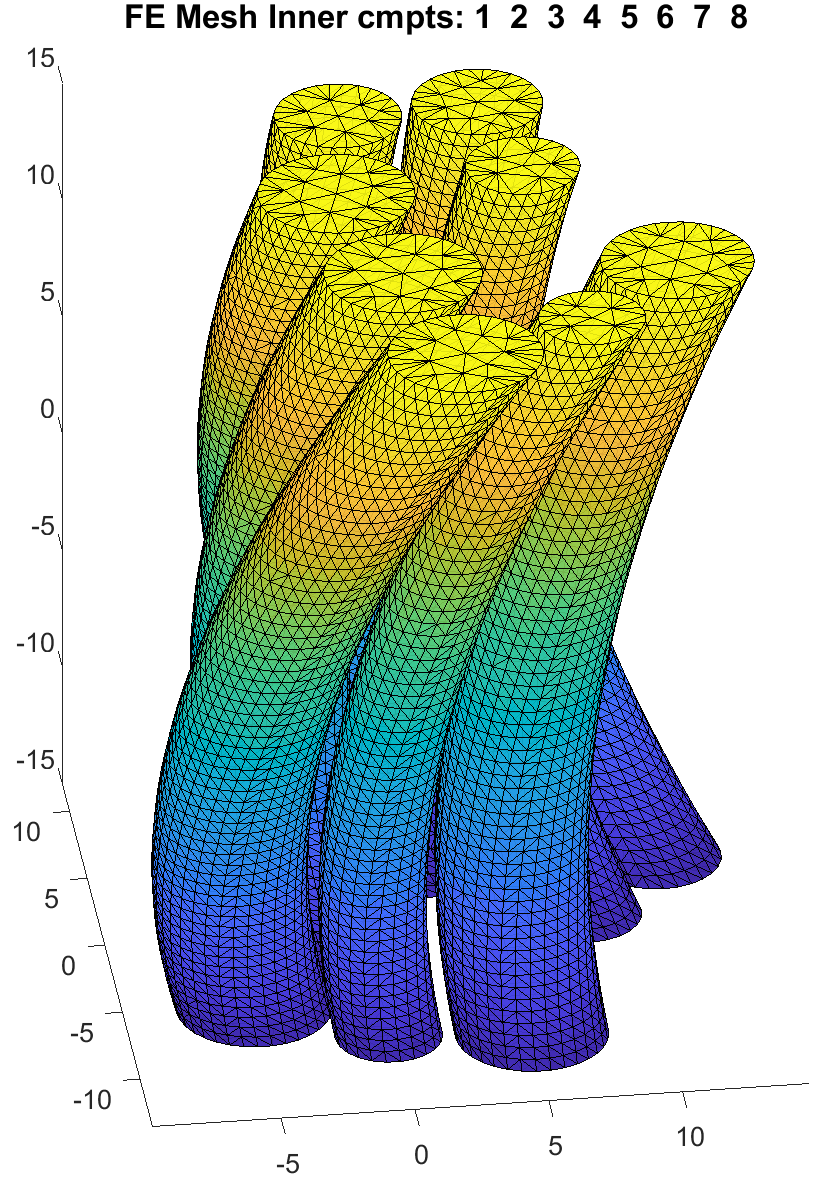
\includegraphics[width=0.3\textwidth]{plot_femesh/cylinders_cells.png}
    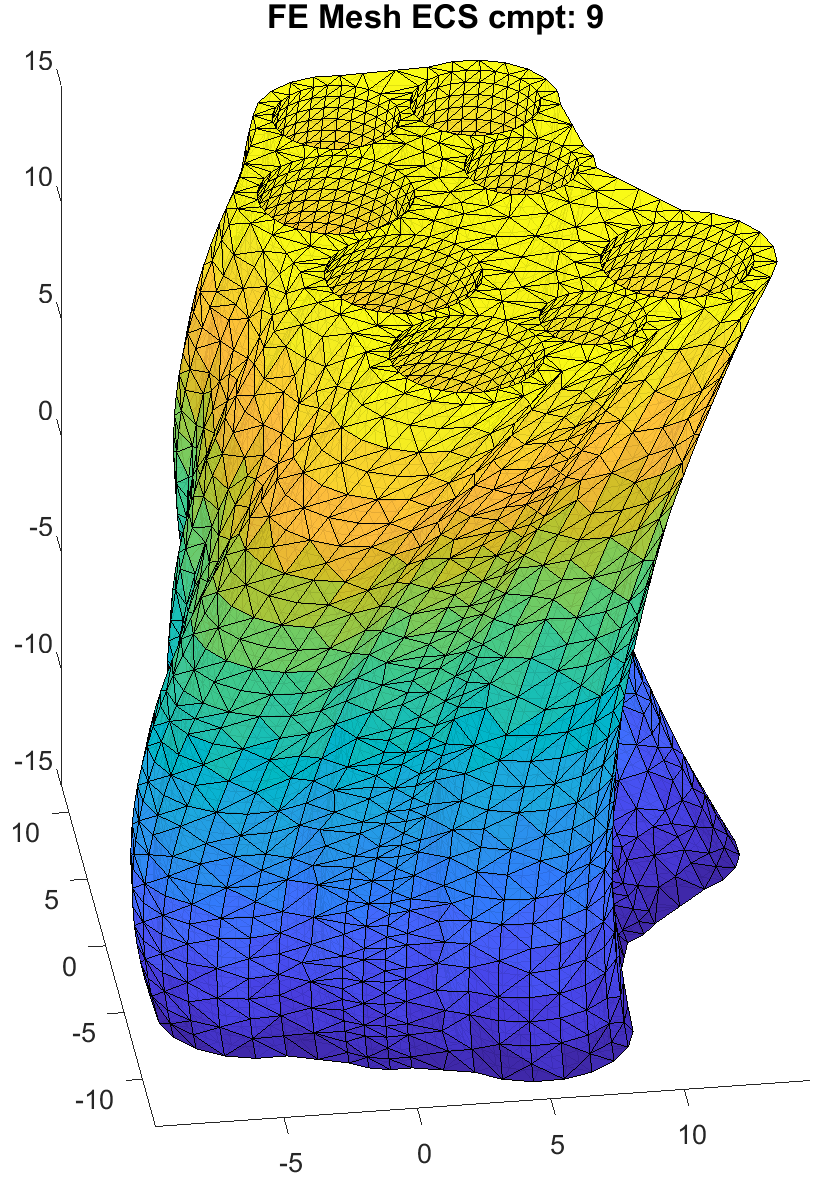
\includegraphics[width=0.3\textwidth]{plot_femesh/cylinders_ecs.png}
    \caption{FE mesh of cylinders and ECS after bending and twisting.
        Compartment number is 1 to 8 for the cylinders and 9 for the ECS.}
    \label{fig:plot_fe_mesh}
\end{figure}



\subsection{Solve BTPDE} \label{sec:solve_btpde}


The BTPDE-solver \verb+solve_btpde+ is triggered by the presence of the field \verb+setup.btpde+. The solver first assembles all the finite element matrices, before it loops over gradient amplitudes $\|\vec{g}\|$ (given by \verb+setup.values+ of type \verb+"g"+, \verb+"q"+ or \verb+"b"+), pulse sequences $f$ (given by \verb+setup.sequences+), and directions $\vec{u}_{\vec{g}}$ (given by \verb+setup.gradient.directions+). The loop is traversed using linear indices, meaning that the three loops are combined into one. If the Parallel Computing Toolbox is available, the loop is parallelized.

For each iteration, the ODE-solver is set up with the appropriate functions and parameters. The ODE is then solved using one of the built-in ODE routines in MATLAB (provided in \verb+setup.btpde.ode_solver+), the default being \verb+ode15s+. Only the final magnetization is stored -- this assures limited memory usage if multiple solver calls are running in parallel. The signal is computed from the final magnetization.

In addition, the time interval $[0, T_\text{echo}]$ is split into multiple subintervals if the sequence $f$ is of type \verb+PGSE+, \verb+DoublePGSE+, \verb+CosOGSE+, or \verb+SinOGSE+. This is done to take advantage of the sequence beeing constant on certain intervals, resulting in a simplified ODE-function and a matrix Jacobian (instead of a time dependent Jacobian). The magnetization at the end of one interval is used as initial conditions for the beginning of the next interval. The computational advantage of this scheme is only visible for iterations that would normally take a long time, especially for higher b-values (higher gradient amplitudes or longer pulses). For lower b-values, this procedure may be slower, when the setup of the ODE-solver is larger compared to the actual time-stepping than for higher b-values.



\subsection{Solve HADC model} \label{sec:solve_hadc}

Similarly, the diffusion equation of the HADC model is discretized using $P_1$ finite elements. The solver is controlled by the field \verb+setup.hadc+, of which the precense triggers the solver \verb+solve_hadc+. The ODE-solver is given by \verb+setup.hadc.ode_solver+ (default: \verb+ode15s+), with tolerances \verb+setup.hadc.abstol+ and \verb+setup.hadc.reltol+.

The solver assembles the finite element matrices \mat{M}, \mat{S}, and \mat{G}, before it loops over compartments, sequences and directions using linear indices, possible using parallel iterations if the Parallel Computing Toolbox is available.

The HADC model differs from the BTDPE in that the compartments are assumed to be separated, and we therefore solve for each compartment separately. The HADC does not depend on the gradient amplitudes $\|\vec{g}\|$. In addition, the HADC solver has to store all the time steps from the ODE-solver, as time integrals are required.

Each iteration consists of setting up the ODE for the diffusion equation for the given sequence $f$ (with integral $F$) and direction $\vec{u}_{\vec{g}}$. The solution to the diffusion equation $\vec{\zeta}(t)$ is computed and stored for all time steps. The integral quantity $\int_0^{T_\text{echo}} F(t) h(t)\, \mathrm{d}t$ is then computed numerically, using a trapezoidal rule with the time steps $t_1, \dots, t_{N_\text{step}}$. The denominator in Eq. \eqref{eq:hadc} is available through the \verb+bvalue_no_q+ method of the sequence.


\subsection{Solve matrix formalism model} \label{sec:solve_mf}

The function \verb+compute_laplace_eig+ computes the Laplace eigenvalues $(\lambda_n)_{n=1, \dots, N_\text{eig}}$, eigenfunction coefficients $\mat{P} \in \mathbb{R}^{N_\text{node} \times N_\text{eig}}$, and first order moments of products of pairs of eigenfunctions $\mat{A}^x$, $\mat{A}^y$, and $\mat{A}^z$, given a length scale $\ell_\text{min}$ and guiding number $N_\text{eig}$. The function \verb+solve_mf+ can then compute the resulting magnetization and signal, using the same parallel looping scheme as for \verb+solve_btpde+ (see Section \ref{sec:solve_btpde}). Once the Laplace eigendecomposition has been performed, computing the the magnetization is straightforward, and generally requires only a fraction of the time it takes to call \verb+solve_btpde+ directly. It does still however requiring assembling the mass matrix for projecting the initial spin density onto the Laplace eigenbasis and computing the signal.


\subsection{Solve analytical model} \label{sec:solve_analytical}

SpinDoctor also allows for solving an analytical multilayer model, based on the article and corresponding code in \cite{grebenkov2010a}. This is a particular form of the previously specified matrix formalism model, where the geometry is assumed to consist of structures only varying in the radial direction, with dimension one (slabs), two (cylinders), or three (spheres). The matrix formalism is reduced to finding radial Laplace eigenvalues and eigenfunctions, providing an analytical solution for the signal attenuation.

The function \verb+solve_analytical+ is triggered by the precense of the field \verb+setup.analytical+. In order to call this function, the geometry has to be of type \verb+"cylinder"+ or \verb+"sphere"+, with $N_\text{cell} = 1$. The geometry can optionally include \verb+"in"+ and/or \verb+"ecs"+ compartments. For cylinders, the axon, myelin, and ECS tops and bottoms are assumed to be reflective, i.e. $\kappa^\text{in} = \kappa^\text{out} = \kappa^\text{ecs} = 0$. For spheres, the outer ECS boundary can have a surface relaxivity $\kappa^\text{ecs} \geq 0$, or if the ECS is not included, the out compartment can have a surface relaxivity $\kappa^\text{out} \geq 0$.

This model assumes a radial gradient direction, which is always the case for a sphere, but requires a gradient direction in the $x$-$y$ plane for cylinders. Currently, only \verb+PGSE+ is supported. The output is $S^\text{ML}(f, \|\vec{g}\|)$, and can be used to compare the signals from other simulations. While the geometry independent finite element approach used in \verb+solve_mf+ has errors from both eigenbasis truncation and finite element discretization, the multilayer approach in \verb+solve_analytical+ only has errors from the eigenvalue truncation. The solver parameters are \verb+setup.analytical.length_scale+ and \verb+setup.analytical.eigstep+, the latter giving the smallest expected distance between to radial eigenvalues $\lambda = \alpha^2$. For eigenvalues that are closer than this distance, only one will be identified. For more information about the spacing between the eigenvalues, consult \cite{grebenkov2010a}.


\subsection{Visualization of results}

To display results in one diffusion-encoding direction, the user can choose the following options:
\begin{enumerate}
    \item the signal is plotted against the b-values;
    \item the ADC is plotted against the geometrical compartment number.
\end{enumerate}
We note that if the ADC from the short time approximation is negative (meaning the short diffusion time assumption is not satisfied), we do not display the negative ADC in the plot.

For results in multiple diffusion-encoding directions uniformly distributed on the three dimensional unit sphere, the user can call the function \verb+plot_hardi+, which plots the signals are plotted as a surface plot. The dots are the end points of the vectors in the diffusion-encoding direction multiplied the signal. The color gives the magnitude of the signal, which can be the signal or the ADC.

The user can also choose to plot the magnetization solution at the surface nodes of the finite elements mesh, using the functions \verb+plot_field+ or \verb+plot_field_everywhere+. These functions can also be used to plot eigenfunctions.



\section{Finite elements meshes of neurons}

The diffusion MRI signal arising from neurons can be numerically simulated by solving the Bloch-Torrey partial differential equation. In order to facilitate the diffusion MRI simulation of realistic neurons by the research community, we constructed finite element meshes for a group of 36 pyramidal neurons and a group of 29 spindle neurons whose morphological descriptions were found in the publicly available neuron repository {\it NeuroMorpho.Org} \cite{NeuronModule}. These finite elements meshes range from having 15163 nodes to 622553 nodes. We also broke the neurons into the soma and dendrite branches and created finite elements meshes for these cell components. Through the Neuron Module, these neuron and components finite element meshes can be seamlessly coupled with the functionalities of SpinDoctor to provide the diffusion MRI signal that can be attributed to spins inside neurons.

As this time, we have not implemented the Neuron Module for coupled compartments linked by permeable membranes. Rather, the diffusion MRI signal is computed with zero permeability on the compartment boundaries. The current emphasis of the Neuron Module is to show how the geometrical structure of neurons affect the diffusion MRI signal. Thus, some of the input parameters related to multiple compartment models in SpinDoctor are not applicable in the current version of the Neuron Module. However, we have kept the exactly same input formats as SpinDoctor in anticipation of the future development of the Neuron Module for permeable membranes. In particular, the various compartments in SpinDoctor have designations as IN, OUT, and ECS, and in the Neuron Module, the geometry defined by the finite element mesh is designated as the OUT compartment.

Table \ref{table:all_neuron_meshes} lists the names and the finite element mesh sizes of the group of 36 pyramidal neurons and the group of 29 spindle neurons. Table \ref{table:morphological} shows the morphological characteristics for the neurons. The neuron models and the measurement data are from \cite{ascoli9247} and \cite{watson2006dendritic}.

\begin{table}
    \begin{tabular}{|c|c|c|c|}
    \hline
    Neuron ID                    & Num of FE mesh nodes & Neuron ID                     & Num of FE mesh nodes \\ \hline
    \textit{03a\_spindle2aFI}    & 38202                & \textit{02a\_pyramidal2aFI}   & 119156               \\ \hline
    \textit{03a\_spindle6aFI}    & 44000                & \textit{02b\_pyramidal1aACC}  & 45216                \\ \hline
    \textit{03b\_spindle4aACC}   & 17370                & \textit{02b\_pyramidal1aFI}   & 105384               \\ \hline
    \textit{03b\_spindle5aACC}   & 26345                & \textit{03a\_pyramidal9aFI}   & 81530                \\ \hline
    \textit{03b\_spindle6aACC}   & 26792                & \textit{03b\_pyramidal2aACC}  & 28183                \\ \hline
    \textit{03b\_spindle7aACC}   & 21618                & \textit{03b\_pyramidal3aACC}  & 27607                \\ \hline
    \textit{04b\_spindle3aFI}    & 51265                & \textit{03b\_pyramidal3aFI}   & 151362               \\ \hline
    \textit{05b\_spindle5aFI}    & 22457                & \textit{03b\_pyramidal4aFI}   & 96177                \\ \hline
    \textit{06b\_spindle8aACC}   & 15163                & \textit{03b\_pyramidal9aFI}   & 66162                \\ \hline
    \textit{07b\_spindle9aACC}   & 54952                & \textit{04a\_pyramidal4aACC}  & 150897               \\ \hline
    \textit{08a\_spindle13aACC}  & 46293                & \textit{04a\_pyramidal5aACC}  & 89256                \\ \hline
    \textit{09o\_spindle7aFI}    & 38992                & \textit{04b\_pyramidal5aFI}   & 95784                \\ \hline
    \textit{09o\_spindle8aFI}    & 60755                & \textit{04b\_pyramidal6aACC}  & 87195                \\ \hline
    \textit{10a\_spindle18aACC}  & 25797                & \textit{04b\_pyramidal6aFI}   & 90482                \\ \hline
    \textit{12a\_spindle19aACC}  & 31841                & \textit{04b\_pyramidal7aACC}  & 622553               \\ \hline
    \textit{12o\_spindle9aFI}    & 29320                & \textit{05a\_pyramidal10aACC} & 201506               \\ \hline
    \textit{13o\_spindle10aFI}   & 43081                & \textit{05a\_pyramidal8aACC}  & 139975               \\ \hline
    \textit{15o\_spindle12aFI}   & 101548               & \textit{05b\_pyramidal7aFI}   & 208203               \\ \hline
    \textit{16o\_spindle13aFI}   & 18266                & \textit{05b\_pyramidal8aFI}   & 124350               \\ \hline
    \textit{19o\_spindle14aFI}   & 25786                & \textit{05b\_pyramidal9aACC}  & 366659               \\ \hline
    \textit{21o\_spindle15aFI}   & 28822                & \textit{06a\_pyramidal11aACC} & 319574               \\ \hline
    \textit{23o\_spindle16aFI}   & 30073                & \textit{06b\_pyramidal10aFI}  & 106808               \\ \hline
    \textit{25o\_spindle17aFI}   & 52919                & \textit{06b\_pyramidal12aACC} & 277718               \\ \hline
    \textit{26o\_spindle18aFI}   & 36239                & \textit{07a\_pyramidal13aACC} & 155854               \\ \hline
    \textit{27o\_spindle19aFI}   & 50807                & \textit{07b\_pyramidal14aACC} & 309789               \\ \hline
    \textit{28o\_spindle20aFI}   & 56036                & \textit{08o\_pyramidal11aFI}  & 419651               \\ \hline
    \textit{28o\_spindle21aFI}   & 17581                & \textit{10a\_pyramidal15aACC} & 56184                \\ \hline
    \textit{29o\_spindle22aFI}   & 18414                & \textit{11a\_pyramidal16aACC} & 222732               \\ \hline
    \textit{30o\_spindle23aFI}   & 26357                & \textit{11o\_pyramidal12aFI}  & 380293               \\ \hline
    \textit{22o\_pyramidal16aFI} & 389878               & \textit{17o\_pyramidal13aFI}  & 326989               \\ \hline
    \textit{24o\_pyramidal17aFI} & 245058               & \textit{18o\_pyramidal14aFI}  & 338453               \\ \hline
    \textit{25o\_pyramidal18aFI} & 71209                & \textit{20o\_pyramidal15aFI}  & 247116               \\ \hline
    \textit{31o\_pyramidal19aFI} & 619390               &                               &                      \\ \hline
\end{tabular}

    \caption{Names and sizes of all the neuron finite elements meshes generated by Tetgen with default settings ($H_\text{tetgen}$ is not defined). The number of FE elements (not shown) is approximately four times the number of FE nodes.}
    \label{table:all_neuron_meshes}
\end{table}

\begin{longtable}{|c|c|c|c|c|c|c|c|c|c|} \hline
	Neuron ID                     & Brain region       & \begin{tabular}[c]{@{}c@{}}Average\\ diam. $(\mu m)$\end{tabular} & \begin{tabular}[c]{@{}c@{}} Height\\ $(\mu m)$\end{tabular} & \begin{tabular}[c]{@{}c@{}}Soma\\ vol. $(\mu m^3)$\end{tabular} & \begin{tabular}[c]{@{}c@{}}Total\\ vol. $(\mu m^3)$\end{tabular} \\ \hline
	\textit{02a\_pyramidal2aFI}   & fronto-insula      & 1.27                      & 404.85                    & 19701.05                  & 25639.61                  \\ \hline
	\textit{02b\_pyramidal1aACC}  & anterior cingulate & 1.58                      & 363.08                    & 9065.56                   & 11579.71                  \\ \hline
	\textit{02b\_pyramidal1aFI}   & fronto-insula      & 1.62                      & 381.56                    & 22475.52                  & 29804.96                  \\ \hline
	\textit{03a\_pyramidal9aFI}   & fronto-insula      & 2.15                      & 532.30                    & 22557.27                  & 30189.28                  \\ \hline
	\textit{03a\_spindle2aFI}     & fronto-insula      & 1.74                      & 387.16                    & 13406.27                  & 17684.23                  \\ \hline
	\textit{03a\_spindle6aFI}     & fronto-insula      & 1.66                      & 501.47                    & 33458.19                  & 37812.72                  \\ \hline
	\textit{03b\_pyramidal2aACC}  & anterior cingulate & 1.48                      & 189.29                    & 2977.21                   & 4487.44                   \\ \hline
	\textit{03b\_pyramidal3aACC}  & anterior cingulate & 1.14                      & 188.45                    & 6005.06                   & 6891.04                   \\ \hline
	\textit{03b\_pyramidal3aFI}   & fronto-insula      & 1.84                      & 496.35                    & 32510.62                  & 46154.08                  \\ \hline
	\textit{03b\_pyramidal4aFI}   & fronto-insula      & 1.33                      & 414.70                    & 35253.85                  & 39324.87                  \\ \hline
	\textit{03b\_pyramidal9aFI}   & fronto-insula      & 1.92                      & 430.06                    & 15263.14                  & 20532.57                  \\ \hline
	\textit{03b\_spindle4aACC}    & anterior cingulate & 1.43                      & 336.33                    & 3098.39                   & 4070.19                   \\ \hline
	\textit{03b\_spindle5aACC}    & anterior cingulate & 1.49                      & 221.52                    & 11925.78                  & 13242.53                  \\ \hline
	\textit{03b\_spindle6aACC}    & anterior cingulate & 1.33                      & 398.36                    & 4027.74                   & 6058.67                   \\ \hline
	\textit{03b\_spindle7aACC}    & anterior cingulate & 1.18                      & 369.51                    & 4982.41                   & 6076.52                   \\ \hline
	\textit{04a\_pyramidal4aACC}  & anterior cingulate & 1.52                      & 705.96                    & 5684.55                   & 13637.33                  \\ \hline
	\textit{04a\_pyramidal5aACC}  & anterior cingulate & 1.86                      & 410.59                    & 15010.43                  & 24648.35                  \\ \hline
	\textit{04b\_pyramidal5aFI}   & fronto-insula      & 1.78                      & 480.13                    & 10312.87                  & 17184.26                  \\ \hline
	\textit{04b\_pyramidal6aACC}  & anterior cingulate & 1.41                      & 465.88                    & 3129.97                   & 7497.12                   \\ \hline
	\textit{04b\_pyramidal6aFI}   & fronto-insula      & 1.56                      & 310.21                    & 14718.05                  & 21708.21                  \\ \hline
	\textit{04b\_pyramidal7aACC}  & anterior cingulate & 1.3                       & 610.42                    & 17060.60                  & 28552.49                  \\ \hline
	\textit{04b\_spindle3aFI}     & fronto-insula      & 2.71                      & 391.14                    & 22569.99                  & 28404.13                  \\ \hline
	\textit{05a\_pyramidal10aACC} & anterior cingulate & 1.74                      & 281.20                    & 16604.06                  & 21826.41                  \\ \hline
	\textit{05a\_pyramidal8aACC}  & anterior cingulate & 1.29                      & 430.37                    & 24709.77                  & 29778.79                  \\ \hline
	\textit{05b\_pyramidal7aFI}   & fronto-insula      & 2.18                      & 281.02                    & 25720.11                  & 32731.05                  \\ \hline
	\textit{05b\_pyramidal8aFI}   & fronto-insula      & 1.66                      & 361.45                    & 32527.06                  & 44679.46                  \\ \hline
	\textit{05b\_pyramidal9aACC}  & anterior cingulate & 1.56                      & 650.60                    & 23948.05                  & 40014.54                  \\ \hline
	\textit{05b\_spindle5aFI}     & fronto-insula      & 2.35                      & 381.88                    & 15383.08                  & 18190.63                  \\ \hline
	\textit{06a\_pyramidal11aACC} & anterior cingulate & 1.46                      & 437.60                    & 17222.02                  & 29995.02                  \\ \hline
	\textit{06b\_pyramidal10aFI}  & fronto-insula      & 1.92                      & 365.18                    & 43127.81                  & 52179.53                  \\ \hline
	\textit{06b\_pyramidal12aACC} & anterior cingulate & 1.52                      & 324.94                    & 17181.33                  & 24931.32                  \\ \hline
	\textit{06b\_spindle8aACC}    & anterior cingulate & 1.92                      & 342.21                    & 18237.49                  & 19462.92                  \\ \hline
	\textit{07a\_pyramidal13aACC} & anterior cingulate & 1.37                      & 325.73                    & 6254.53                   & 8738.01                   \\ \hline
	\textit{07b\_pyramidal14aACC} & anterior cingulate & 1.67                      & 350.40                    & 16053.07                  & 22772.96                  \\ \hline
	\textit{07b\_spindle9aACC}    & anterior cingulate & 1.75                      & 437.87                    & 21344.83                  & 27307.48                  \\ \hline
	\textit{08a\_spindle13aACC}   & anterior cingulate & 1.74                      & 814.45                    & 9911.07                   & 14113.32                  \\ \hline
	\textit{08o\_pyramidal11aFI}  & fronto-insula      & 1.91                      & 421.68                    & 11512.38                  & 24326.94                  \\ \hline
	\textit{09o\_spindle7aFI}     & fronto-insula      & 2.90                      & 472.87                    & 22052.10                  & 27905.89                  \\ \hline
	\textit{09o\_spindle8aFI}     & fronto-insula      & 2.05                      & 376.73                    & 11923.76                  & 15189.32                  \\ \hline
	\textit{10a\_pyramidal15aACC} & anterior cingulate & 1.40                      & 341.48                    & 8522.11                   & 10960.84                  \\ \hline
	\textit{10a\_spindle18aACC}   & anterior cingulate & 1.57                      & 457.90                    & 5895.17                   & 7219.28                   \\ \hline
	\textit{11a\_pyramidal16aACC} & anterior cingulate & 1.27                      & 486.31                    & 8807.01                   & 12263.84                  \\ \hline
	\textit{11o\_pyramidal12aFI}  & fronto-insula      & 1.91                      & 369.34                    & 70786.62                  & 79516.92                  \\ \hline
	\textit{12a\_spindle19aACC}   & anterior cingulate & 2.05                      & 431.22                    & 12178.08                  & 15618.67                  \\ \hline
	\textit{12o\_spindle9aFI}     & fronto-insula      & 3.41                      & 305.31                    & 29983.79                  & 36678.18                  \\ \hline
	\textit{13o\_spindle10aFI}    & fronto-insula      & 2.69                      & 516.92                    & 39866.55                  & 46022.15                  \\ \hline
	\textit{15o\_spindle12aFI}    & fronto-insula      & 3.60                      & 604.57                    & 53192.65                  & 79170.43                  \\ \hline
	\textit{16o\_spindle13aFI}    & fronto-insula      & 2.17                      & 364.66                    & 17467.88                  & 18888.13                  \\ \hline
	\textit{17o\_pyramidal13aFI}  & fronto-insula      & 1.89                      & 340.77                    & 11004.30                  & 21167.19                  \\ \hline
	\textit{18o\_pyramidal14aFI}  & fronto-insula      & 1.74                      & 288.41                    & 69851.56                  & 78999.20                  \\ \hline
	\textit{19o\_spindle14aFI}    & fronto-insula      & 2.18                      & 232.21                    & 10507.15                  & 12905.43                  \\ \hline
	\textit{20o\_pyramidal15aFI}  & fronto-insula      & 1.82                      & 383.18                    & 22344.32                  & 27667.19                  \\ \hline
	\textit{21o\_spindle15aFI}    & fronto-insula      & 2.36                      & 286.33                    & 17567.69                  & 29466.53                  \\ \hline
	\textit{22o\_pyramidal16aFI}  & fronto-insula      & 1.94                      & 585.35                    & 18776.05                  & 29441.43                  \\ \hline
	\textit{23o\_spindle16aFI}    & fronto-insula      & 1.67                      & 420.05                    & 10429.13                  & 13482.93                  \\ \hline
	\textit{24o\_pyramidal17aFI}  & fronto-insula      & 2.04                      & 371.99                    & 40986.40                  & 47377.09                  \\ \hline
	\textit{25o\_pyramidal18aFI}  & fronto-insula      & 1.80                      & 364.05                    & 18587.13                  & 23572.15                  \\ \hline
	\textit{25o\_spindle17aFI}    & fronto-insula      & 1.79                      & 358.70                    & 7897.44                   & 13563.26                  \\ \hline
	\textit{26o\_spindle18aFI}    & fronto-insula      & 2.27                      & 442.65                    & 52911.93                  & 56084.44                  \\ \hline
	\textit{27o\_spindle19aFI}    & fronto-insula      & 1.73                      & 275.08                    & 20640.14                  & 25423.96                  \\ \hline
	\textit{28o\_spindle20aFI}    & fronto-insula      & 3.00                      & 520.69                    & 35442.59                  & 51267.07                  \\ \hline
	\textit{28o\_spindle21aFI}    & fronto-insula      & 2.62                      & 298.57                    & 35579.06                  & 37783.31                  \\ \hline
	\textit{29o\_spindle22aFI}    & fronto-insula      & 3.52                      & 402.84                    & 62928.22                  & 83279.12                  \\ \hline
	\textit{31o\_pyramidal19aFI}  & fronto-insula      & 2.26                      & 303.55                    & 65950.80                  & 86376.72                  \\ \hline
	\caption{The morphological characteristics of the neurons.} \label{table:morphological}
\end{longtable}


As an illustration, we show the finite elements meshes of 4 spindle neurons in Figure \ref{fig:spindle_neurons}, and in Figure \ref{fig:pyramidal_neurons} we show the finite elements meshes of 4 pyramidal neurons.
\begin{figure}
    \centering
    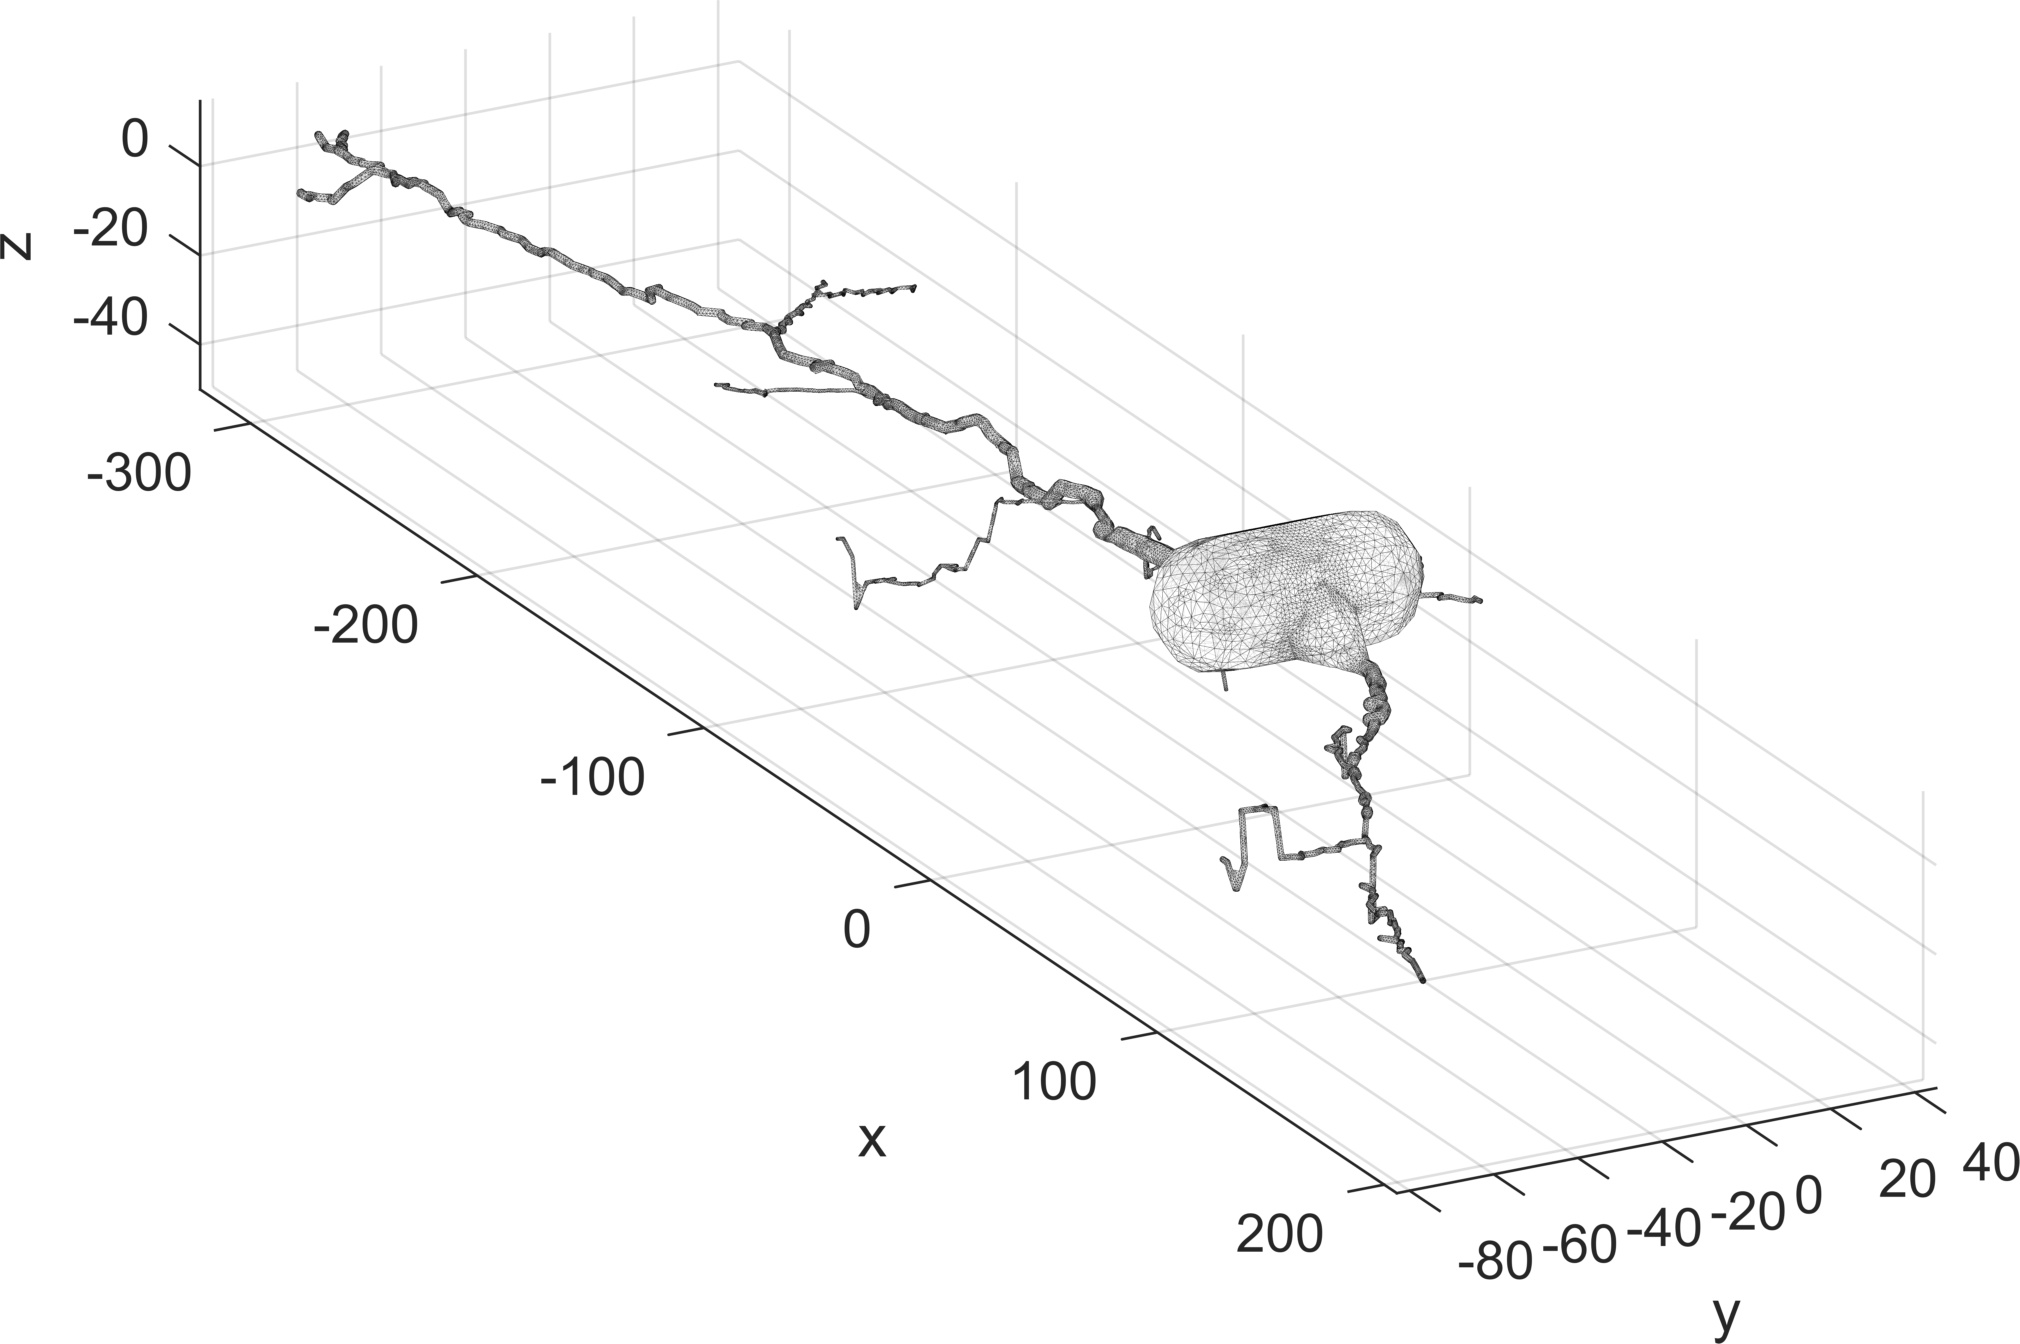
\includegraphics[width=0.45\textwidth]{paper_neuron/03a_spindle6aFI.jpg}
    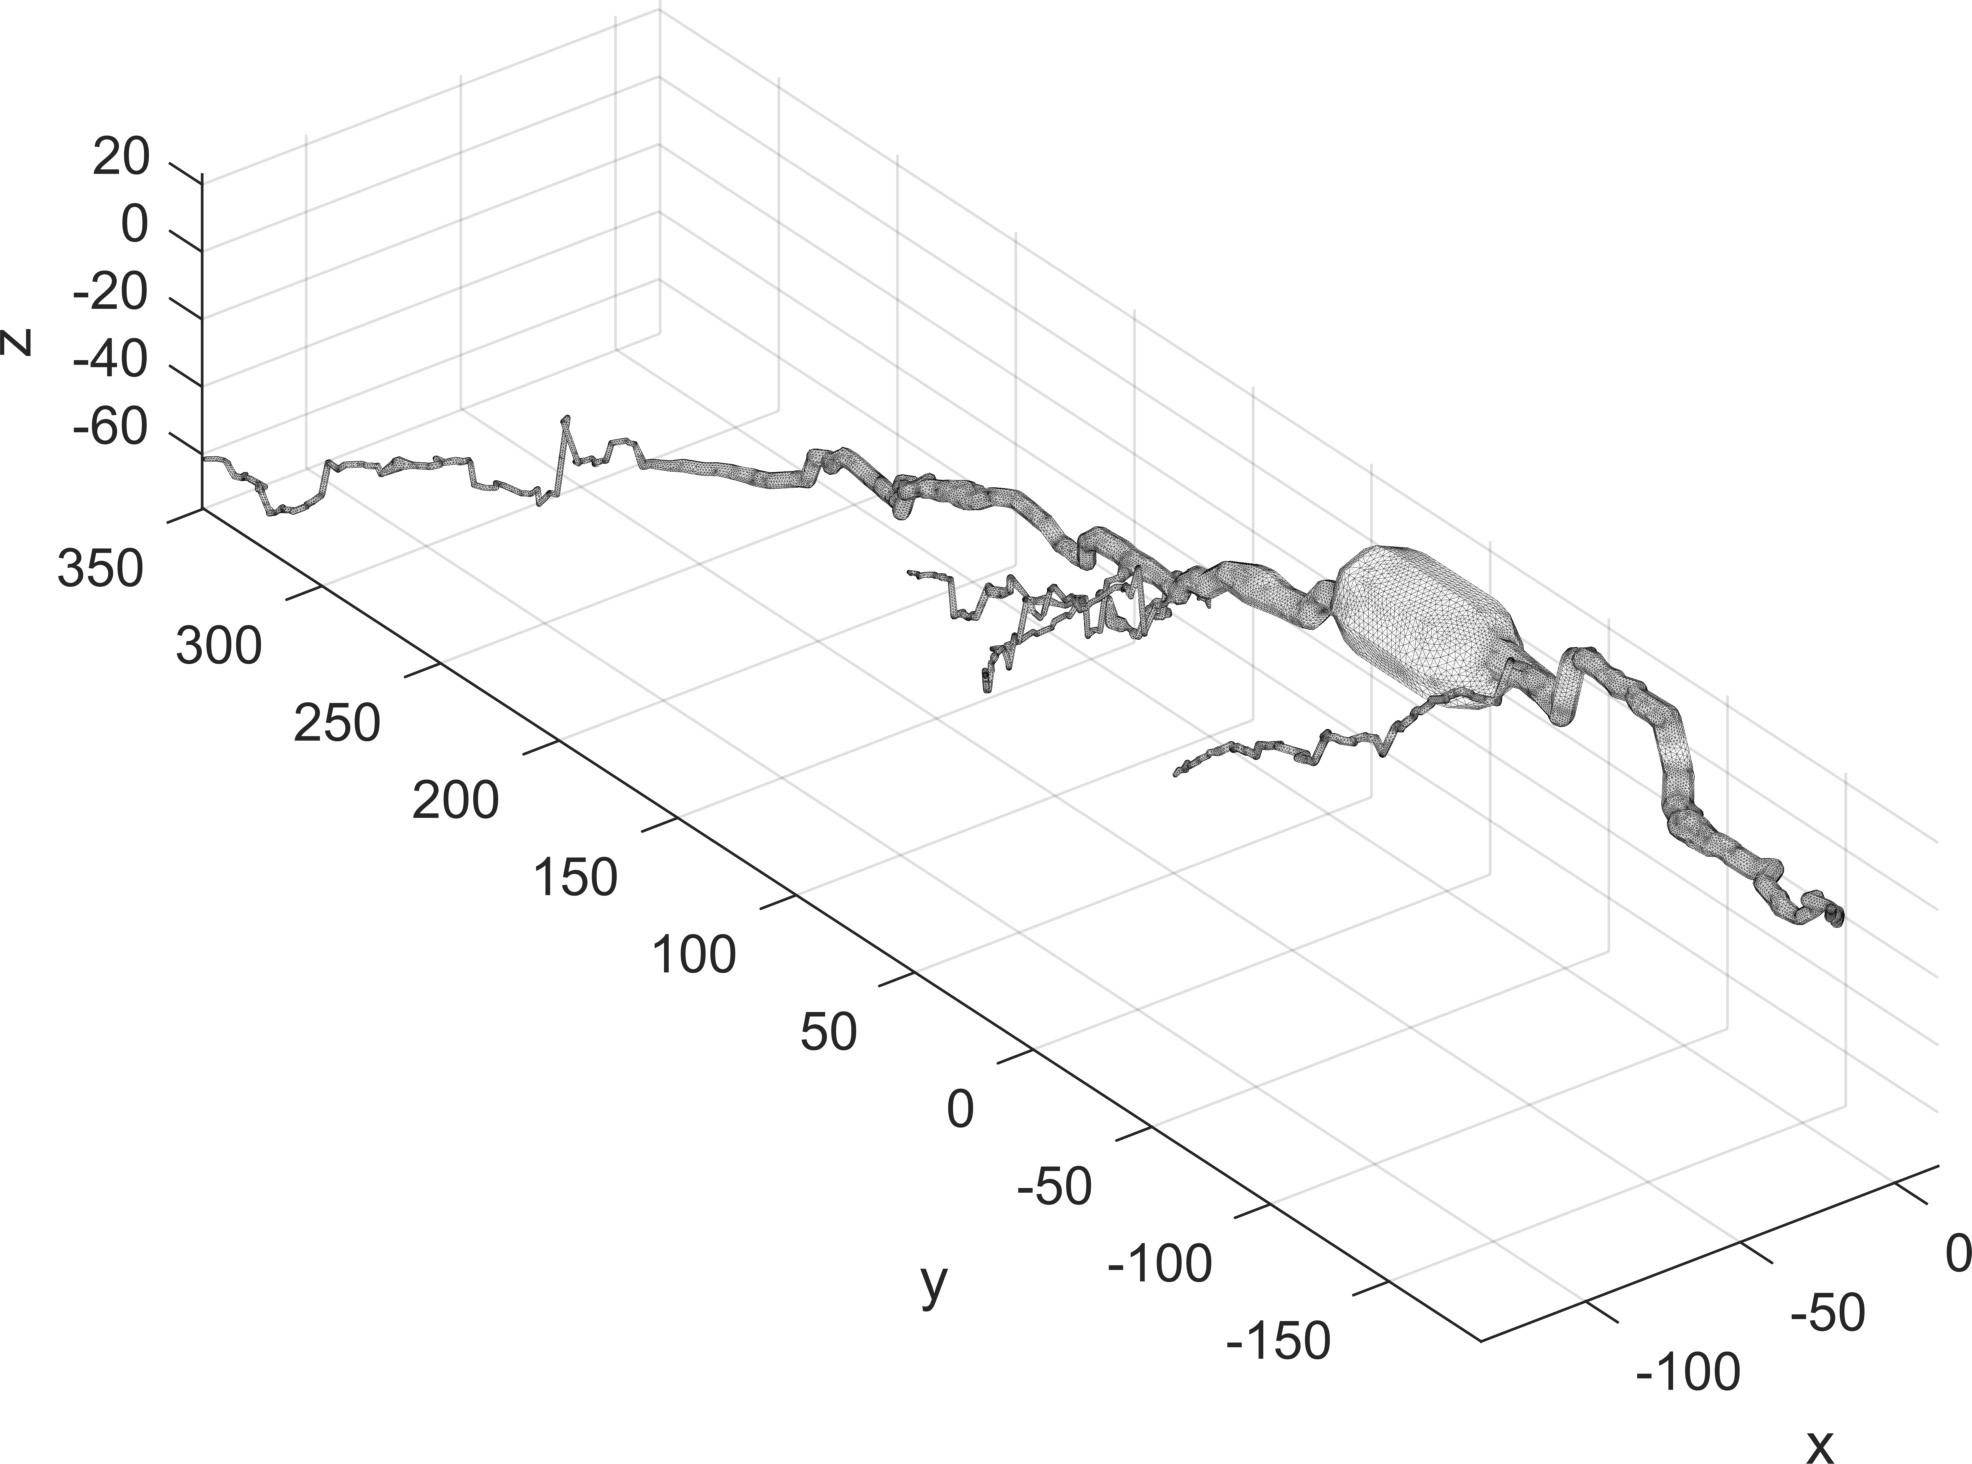
\includegraphics[width=0.45\textwidth]{paper_neuron/28o_spindle20aFI.jpg} \\
    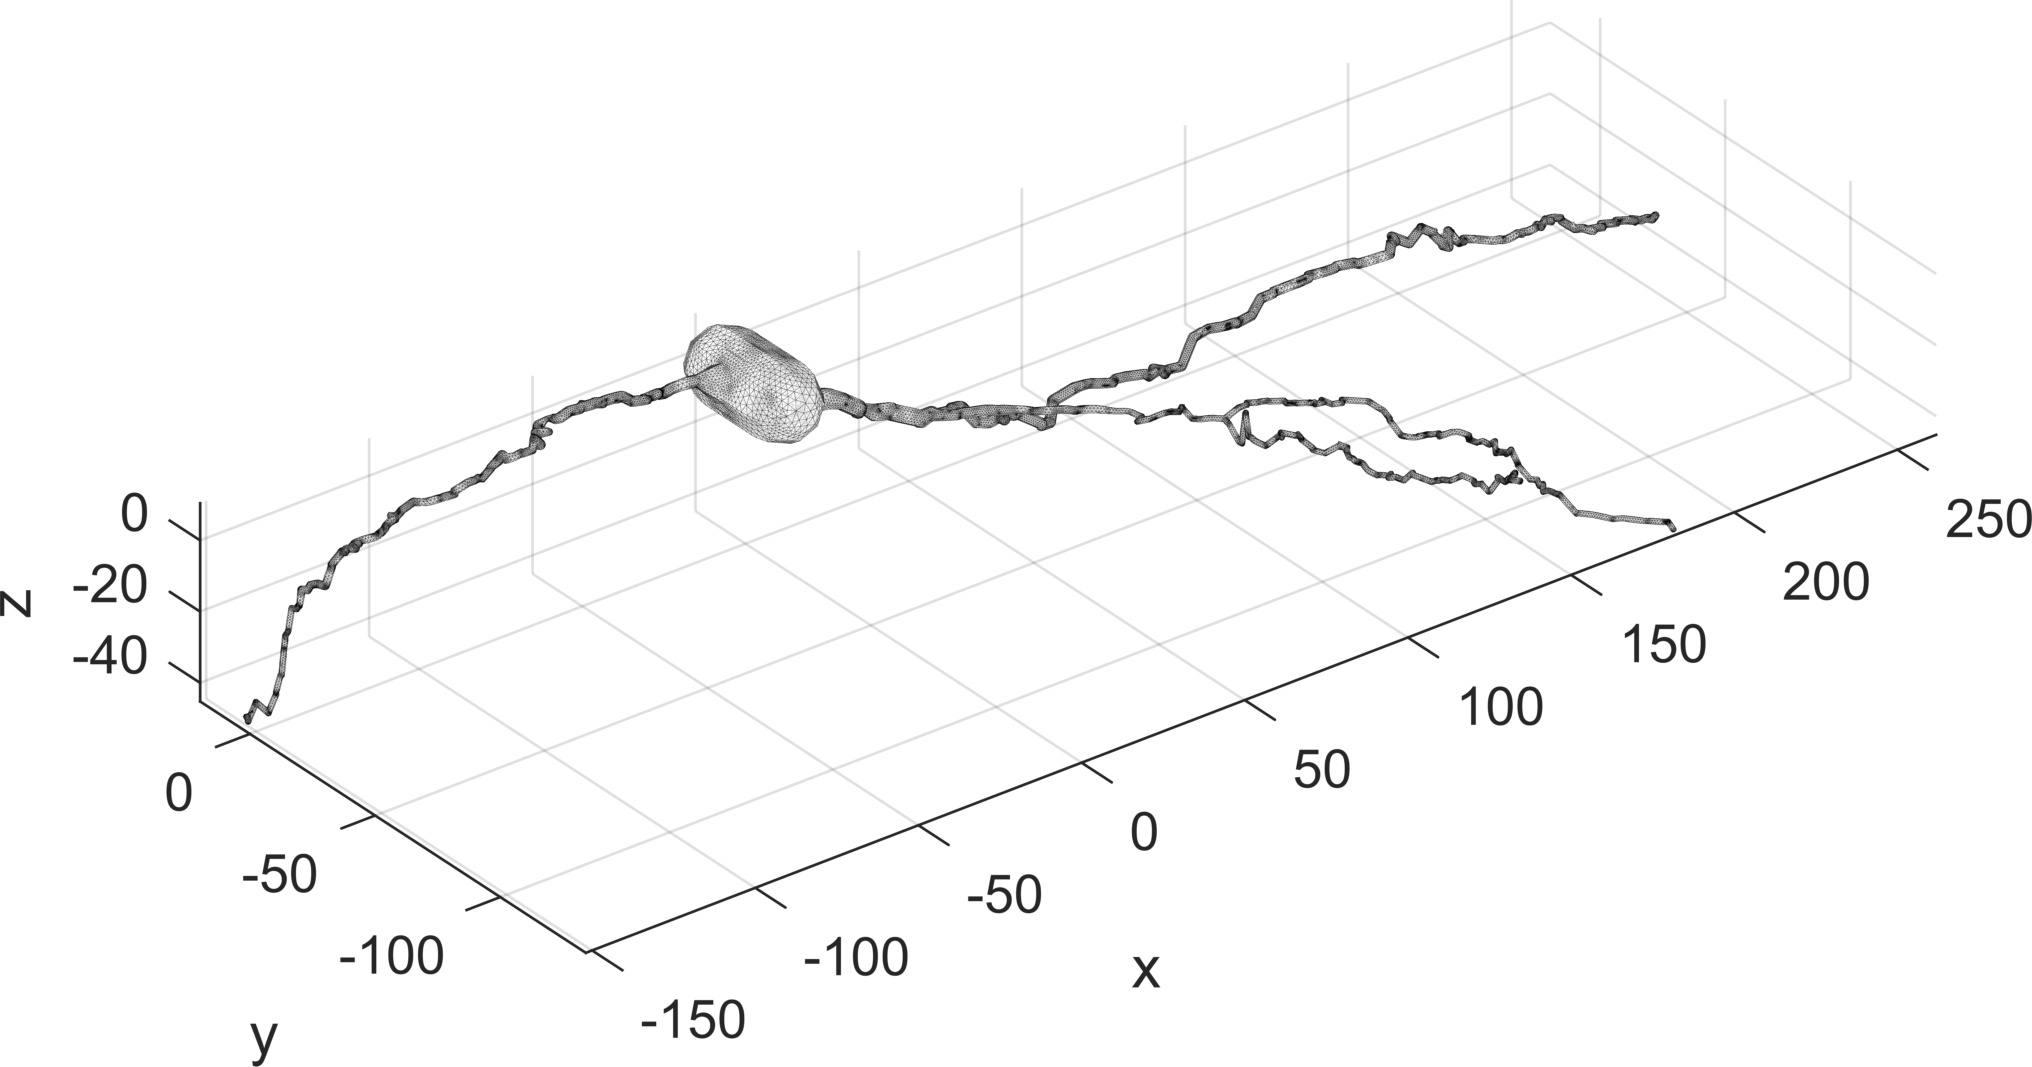
\includegraphics[width=0.45\textwidth]{paper_neuron/09o_spindle8aFI.jpg}
    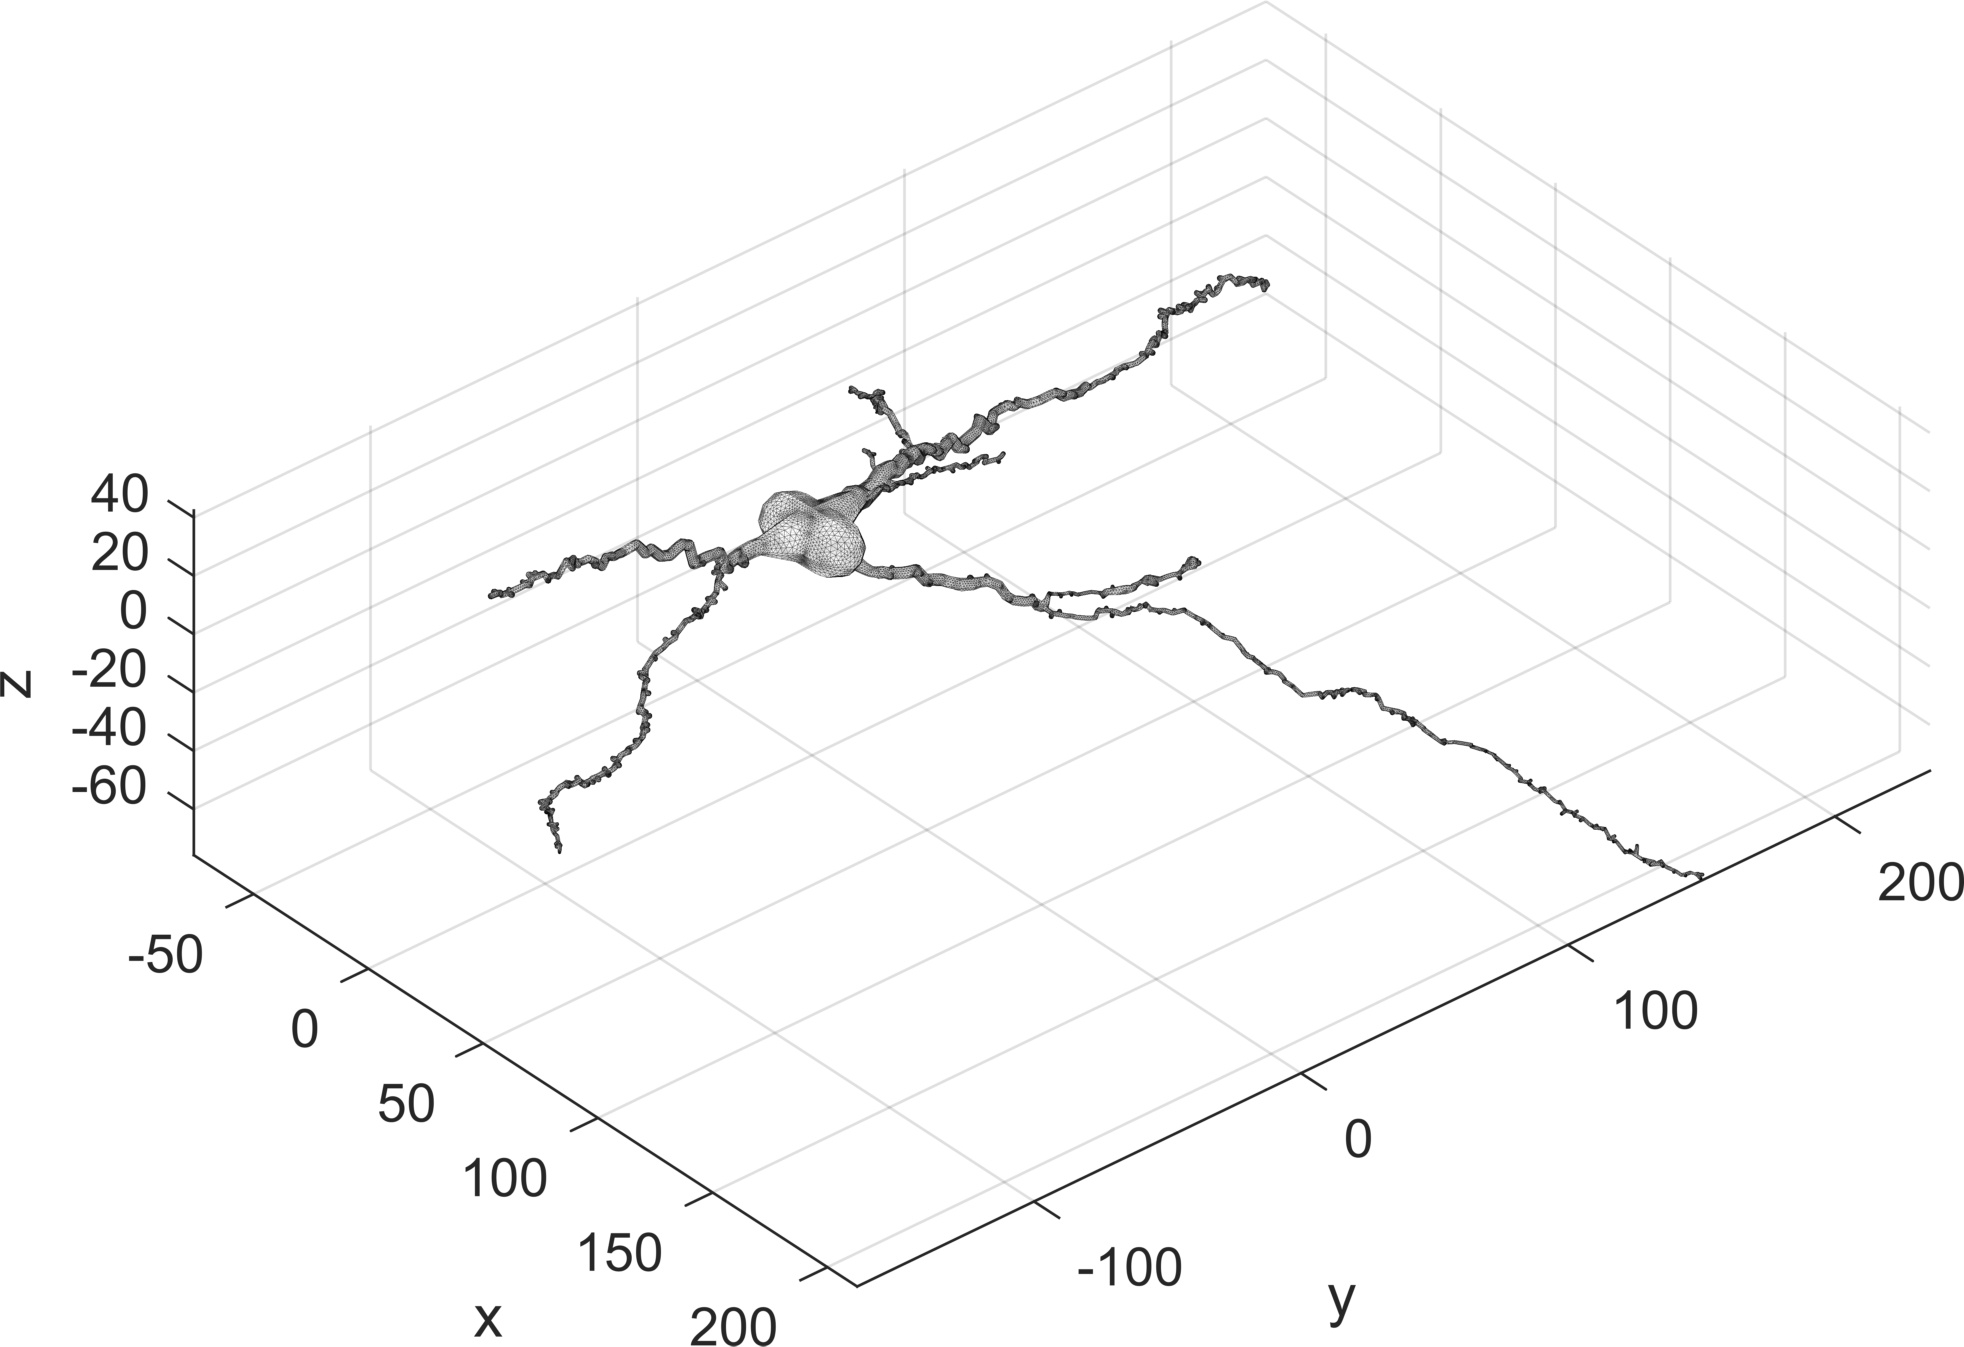
\includegraphics[width=0.45\textwidth]{paper_neuron/25o_spindle17aFI.jpg}
    \caption{The finite elements meshes of four spindle neurons. The unit is \lunit. Top left: {\it 03a\_spindle6aFI}. Top right: {\it 28o\_spindle20aFI}. Bottom left: {\it 09o\_spindle8aFI}. Bottom right: {\it 25o\_spindle17aFI}.}
    \label{fig:spindle_neurons}
\end{figure}

\begin{figure}
    \centering
    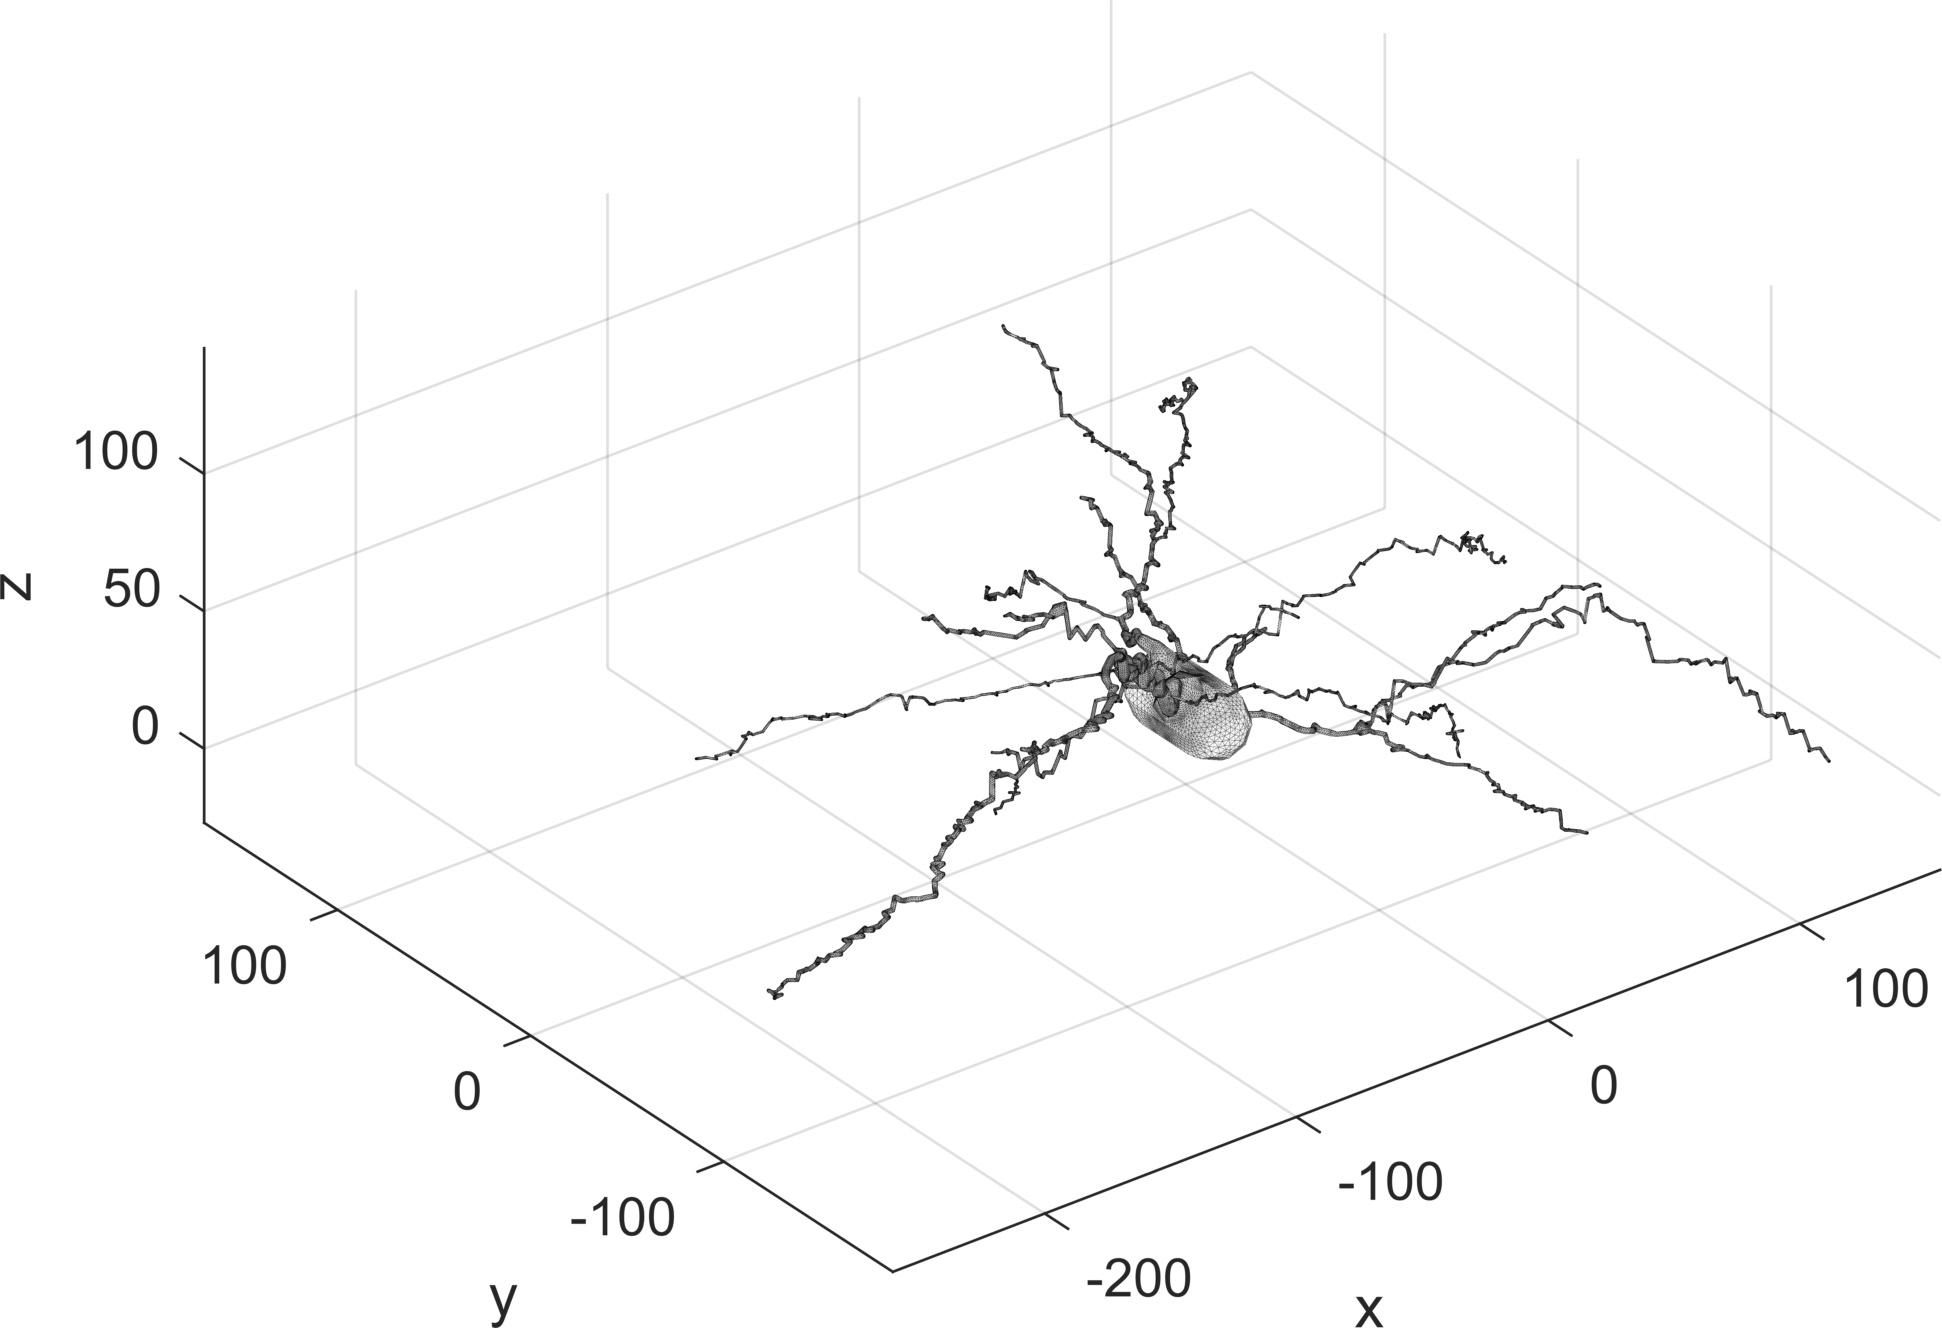
\includegraphics[width=0.45\textwidth]{paper_neuron/02a_pyramidal2aFI.jpg}
    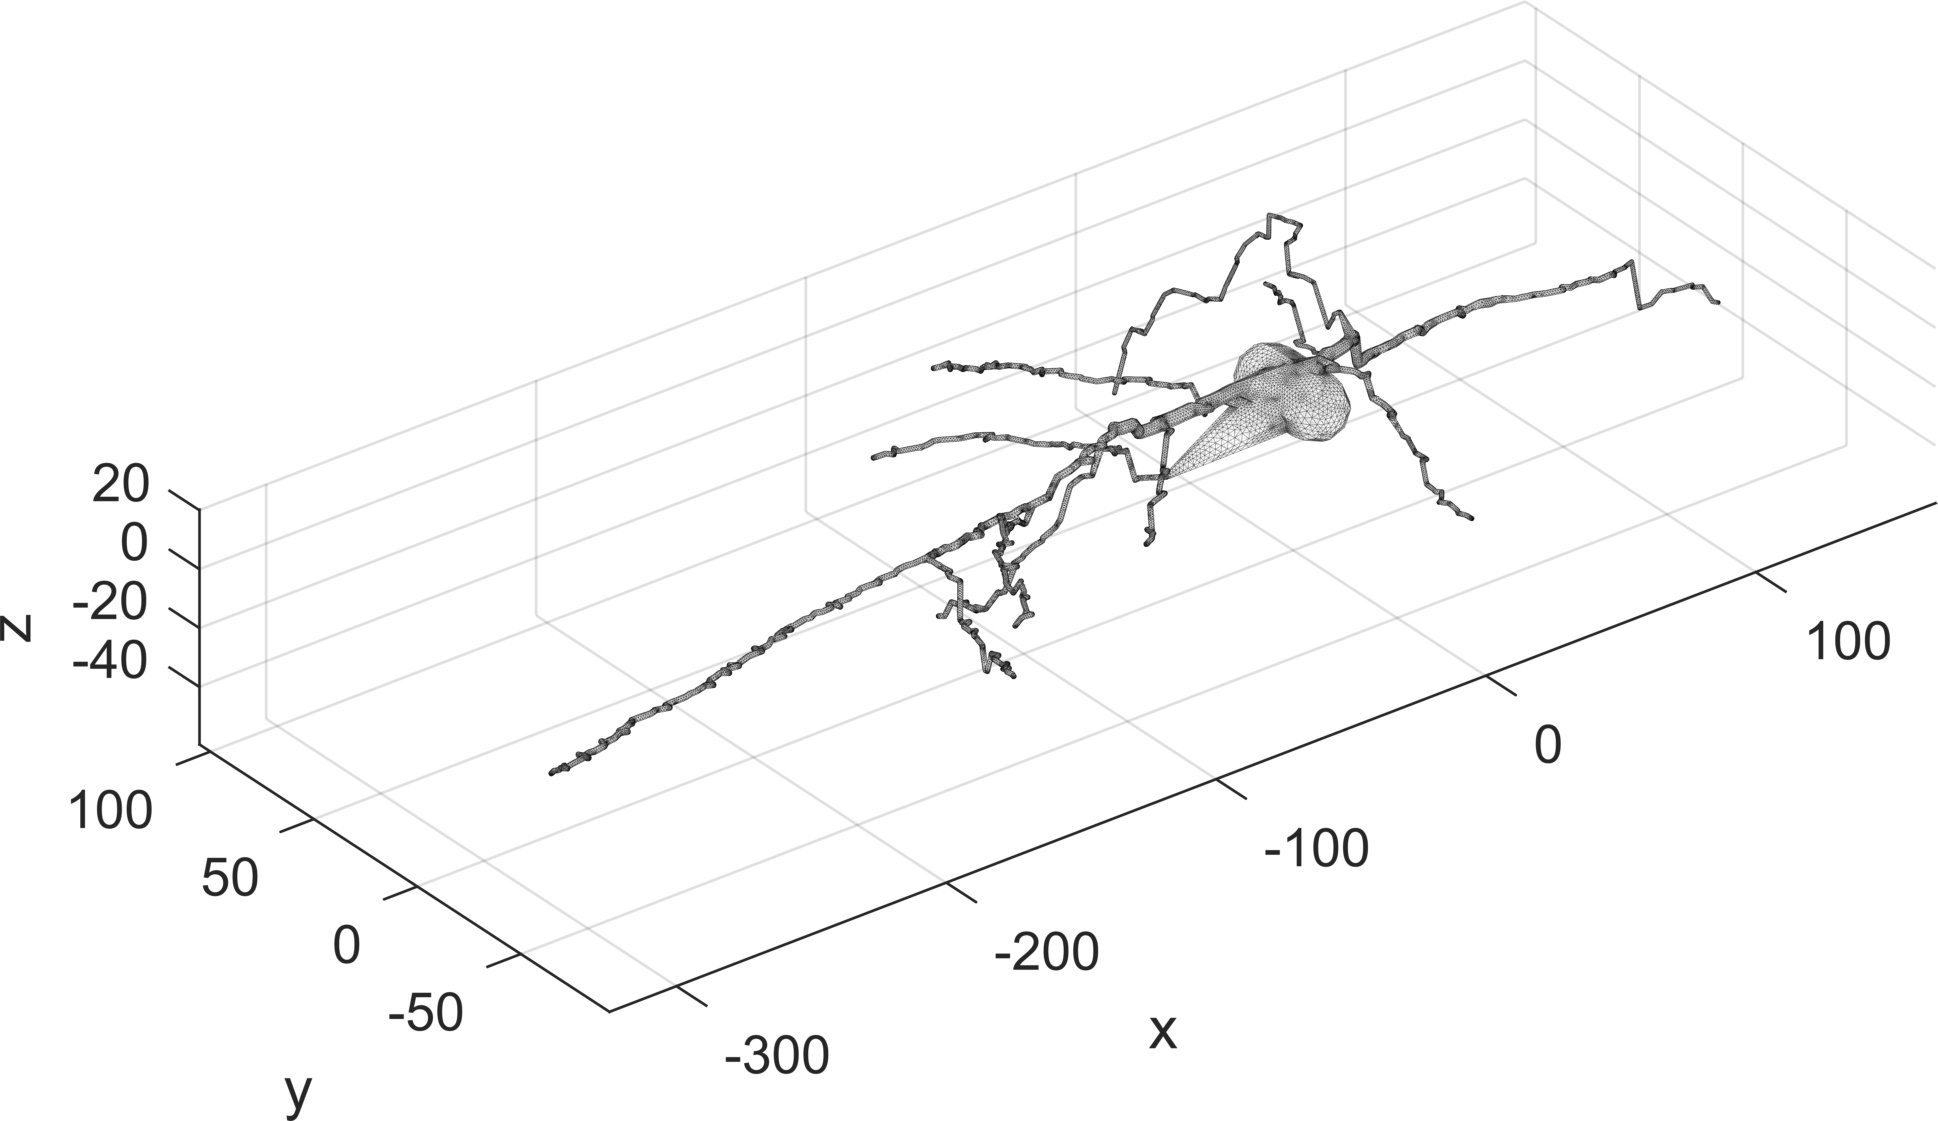
\includegraphics[width=0.45\textwidth]{paper_neuron/03b_pyramidal9aFI.jpg} \\
    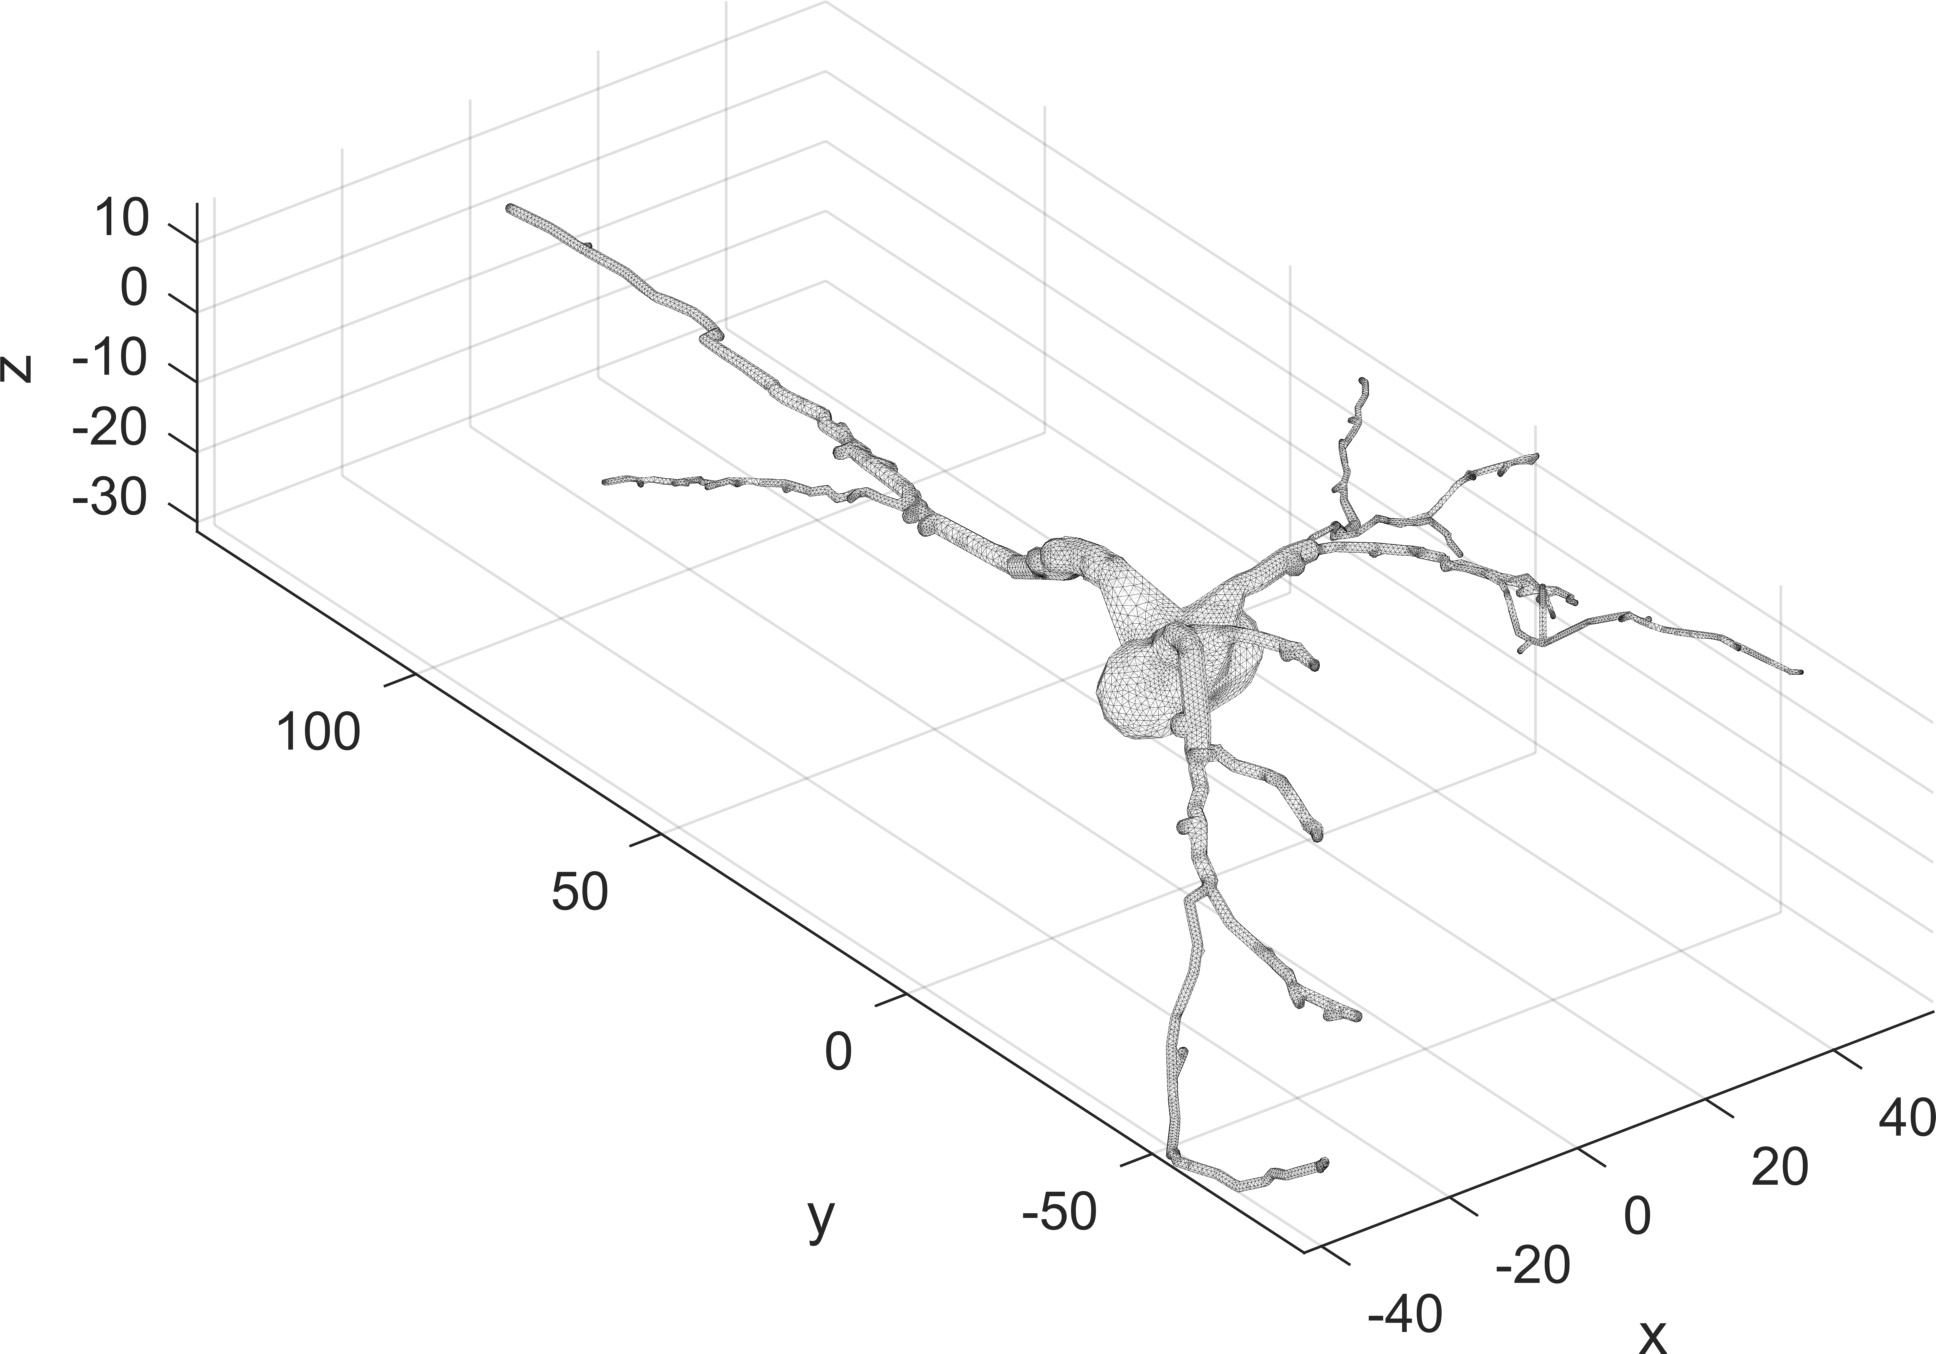
\includegraphics[width=0.45\textwidth]{paper_neuron/03b_pyramidal2aACC.jpg}
    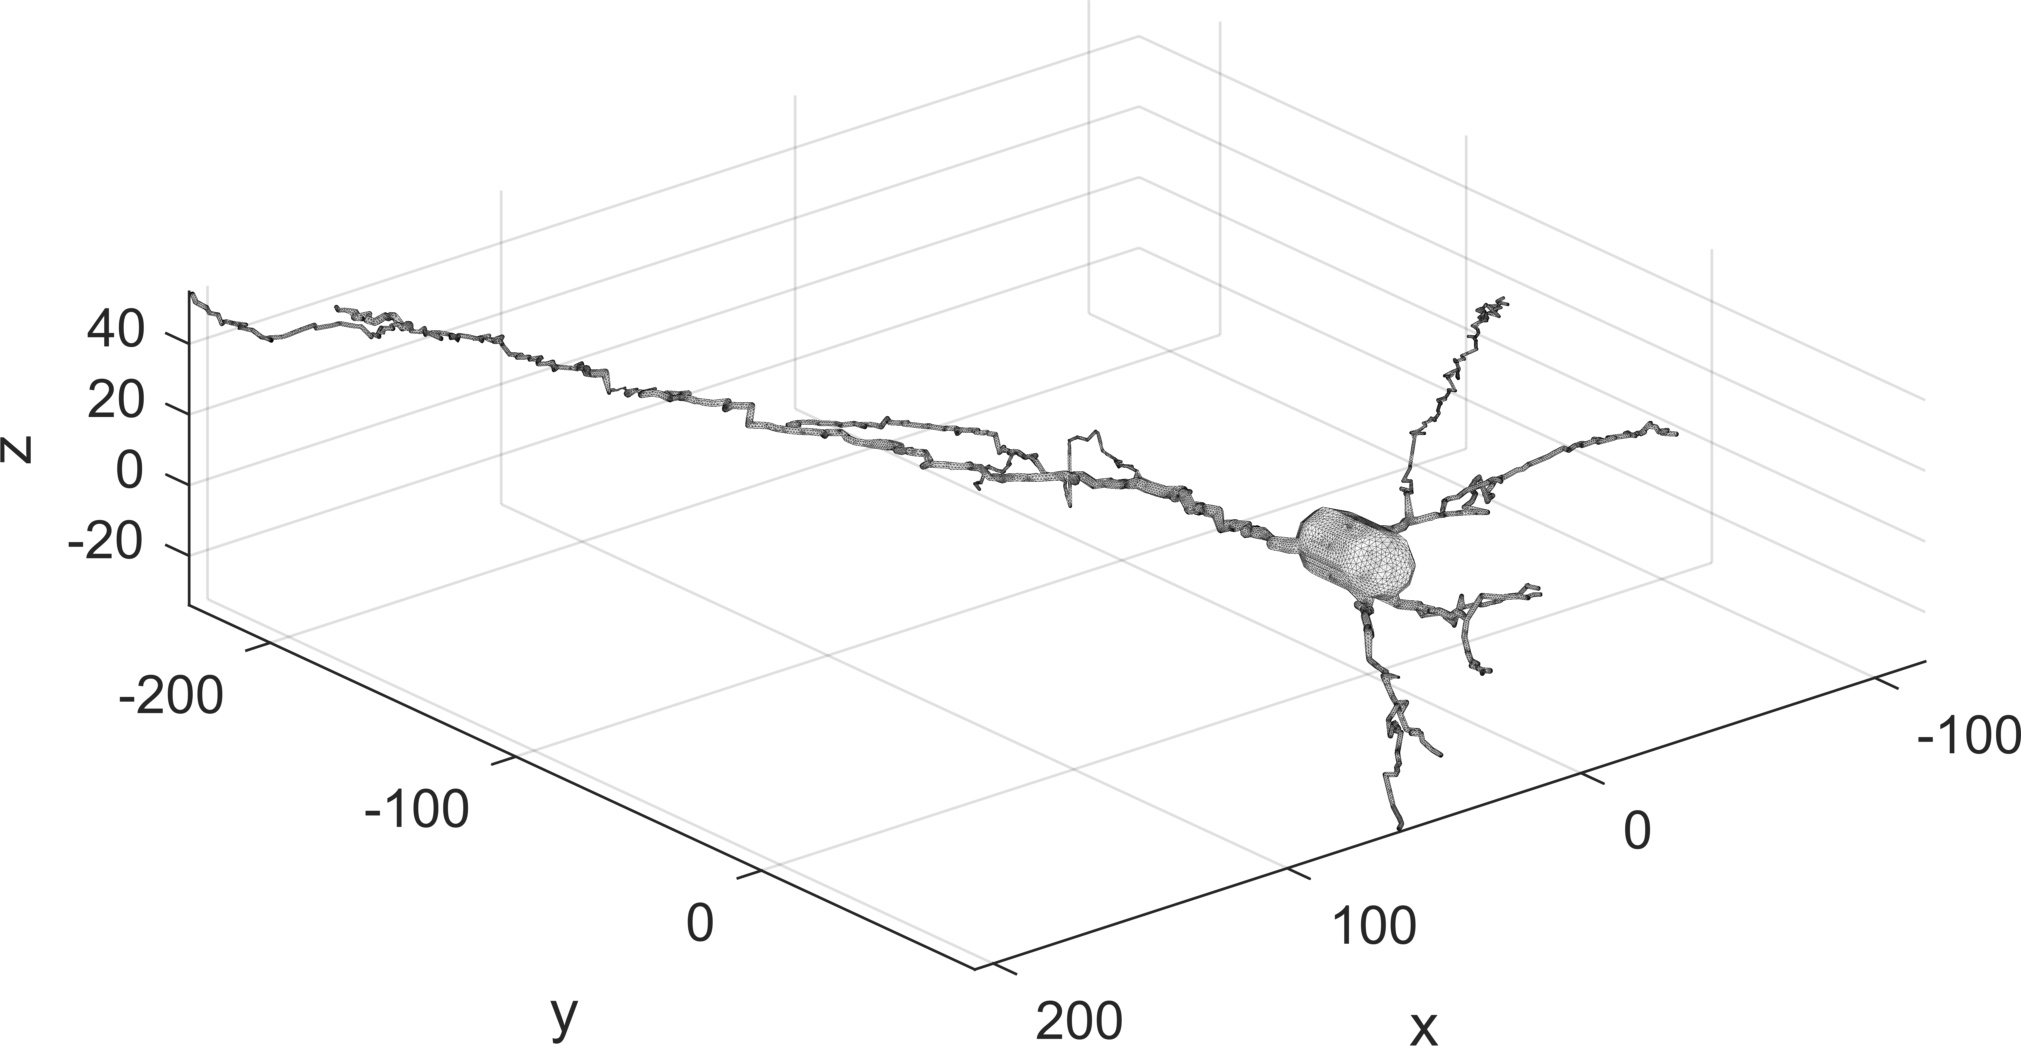
\includegraphics[width=0.45\textwidth]{paper_neuron/10a_pyramidal15aACC.jpg}
    \caption{The finite elements meshes of four pyramidal neurons. The unit is \lunit. Top left: {\it 02a\_pyramidal2aFI}. Top right: {\it 03b\_pyramidal9aFI}. Bottom left: {\it 03b\_pyramidal2aACC}. Bottom right: {\it 10a\_pyramidal15aACC}.}
    \label{fig:pyramidal_neurons}
\end{figure}





\clearpage

\section{SpinDoctor examples}

In this section we show some prototypical examples using the available functionalities of SpinDoctor.



\subsection{Comparison of BTPDE and HADC with Short Time Approximation}

In Fig. \ref{fig:STA} we show that both BTPDE and HADC solutions match the STA values at short diffusion times for cylindrical cells (compartments 1 to 5). We also show that for the ECS (compartment 6), the STA is too low, because it does not account for the fact that spins in the ECS can diffuse around several cylinders. This also shows that when the interfaces are impermeable, the BTPDE ADC and that from the HADC model are identical. The diffusion-encoding sequence here is cosine OGSE with 6 periods.

\begin{figure}
    \centering
    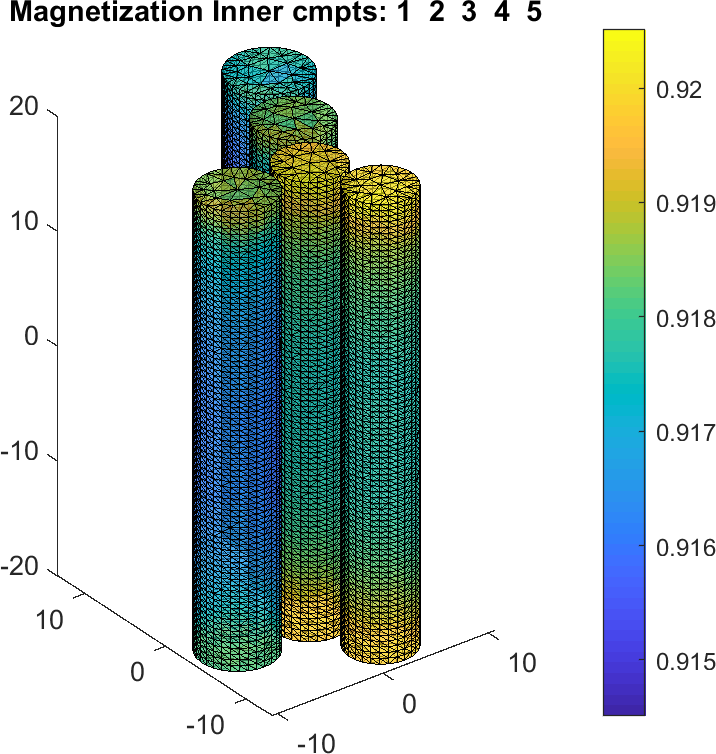
\includegraphics[width=0.35\textwidth]{plot_magnetization/sec42_in.png} \quad
    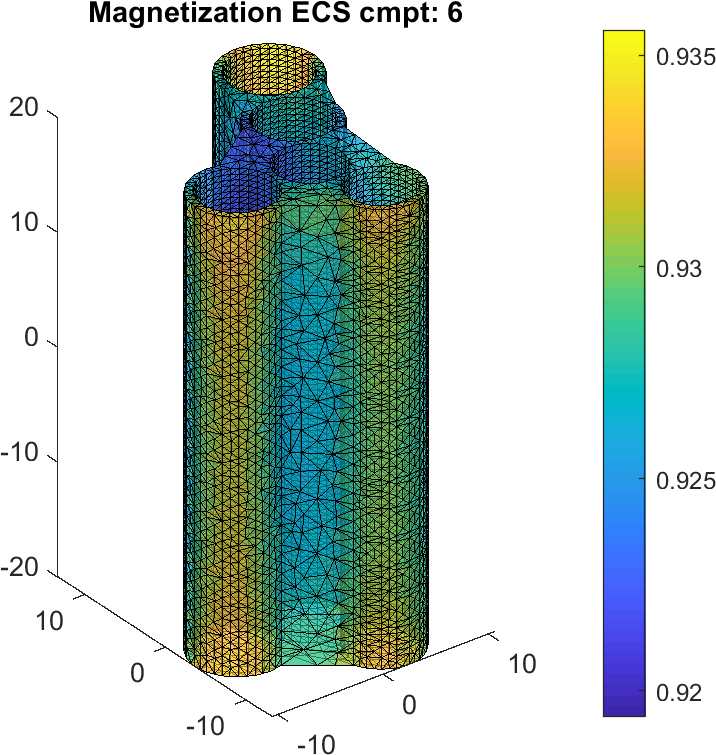
\includegraphics[width=0.35\textwidth]{plot_magnetization/sec42_ecs.png} \\
    \vspace{0.8cm}
    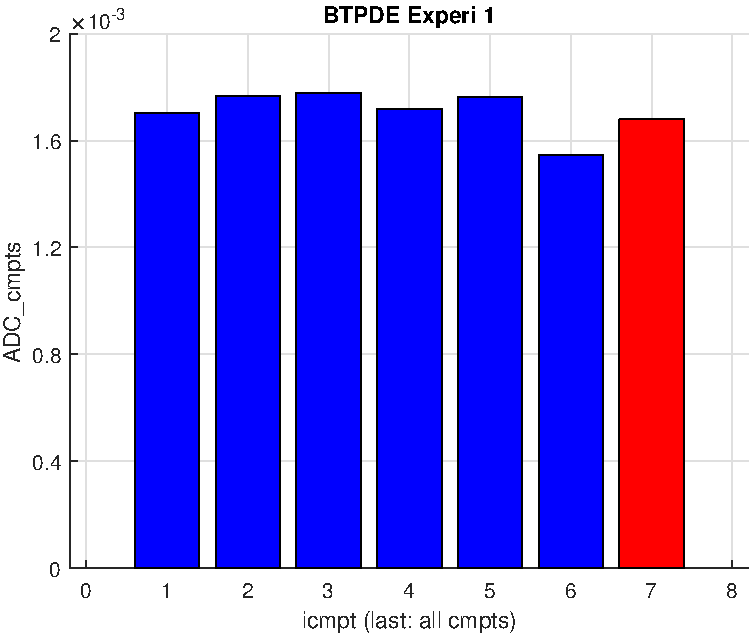
\includegraphics[width=0.32\textwidth]{plot_adc/btpde_sec42.pdf}
    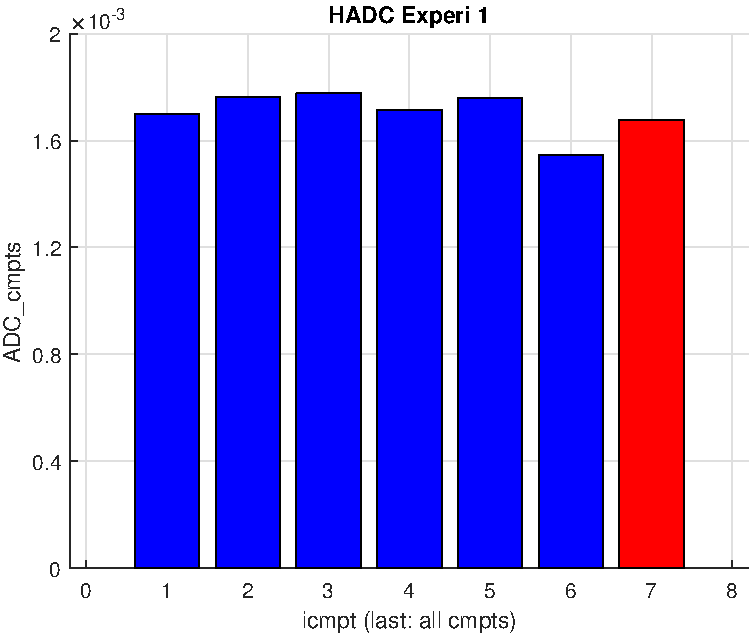
\includegraphics[width=0.32\textwidth]{plot_adc/hadc_sec42.pdf}
    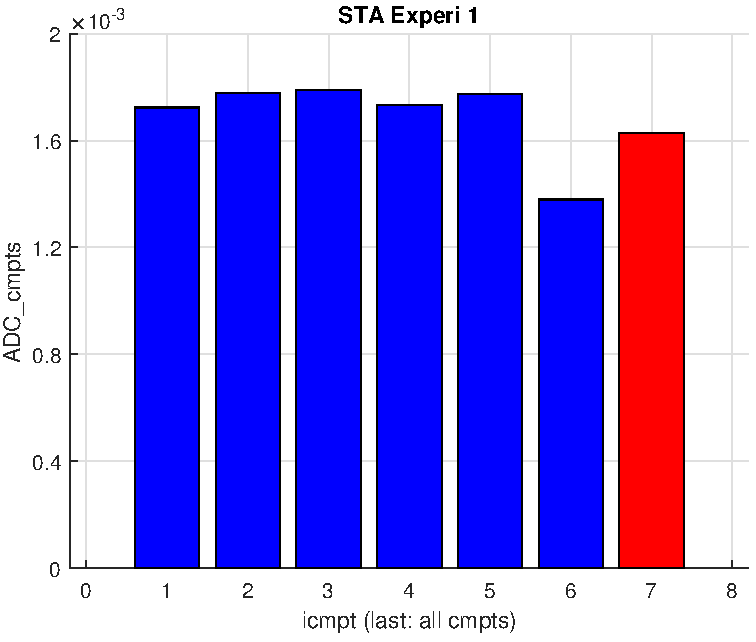
\includegraphics[width=0.32\textwidth]{plot_adc/sta_sec42.pdf}
    \caption{Geometry: 5 cylinders, tight wrap ECS, ecs\_gap = 0.2, $\vec{u}_{\vec{g}}=(1,1,1)^\transpose / \sqrt{3}$, $\sigma^\text{out}=\sigma^{ecs}=2\times10^{-3}\dunit$, $\kappa=0\kunit$, OGSE cosine ($\delta=14\tunit,\Delta=14\tunit$, nperiod = 6). The vertical bars indicate the ADC in each compartment. The ADC in the rightmost position is the ADC that takes into account the diffusion in all the compartments.}
    \label{fig:STA}
\end{figure}





\subsection{Permeable membranes}

In Fig. \ref{fig:perm} we show the effect of permeability: the Bloch-Torrey PDE model includes permeable membranes ($\kappa = 1\e{-3}\kunit$) whereas the HADC has impermeable membranes. We see in the permeable case, the ADC in the spheres are higher than in the impermeable case, whereas the ECS show reduced ADC because the faster diffusing spins in the ECS are allowed to move into the slowly diffusing spherical cells. We note that in the permeable case, the ADC in each compartment is obtained by using the fitting formula involving the logarithm of the dMRI signal, and we defined the ``signal'' in a compartment as the total magnetization in that compartment at $T_\text{echo}$, which is just the integral of the solution of the Bloch-Torrey PDE in that compartment.

\begin{figure}
    \centering
    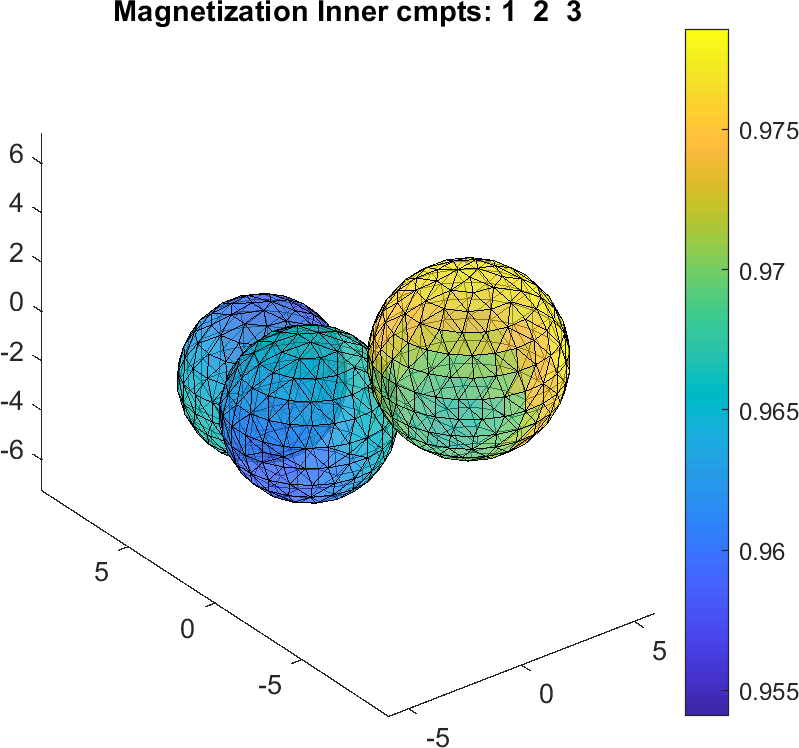
\includegraphics[width=0.35\textwidth]{plot_magnetization/3sph_cells_perm.png} \quad
    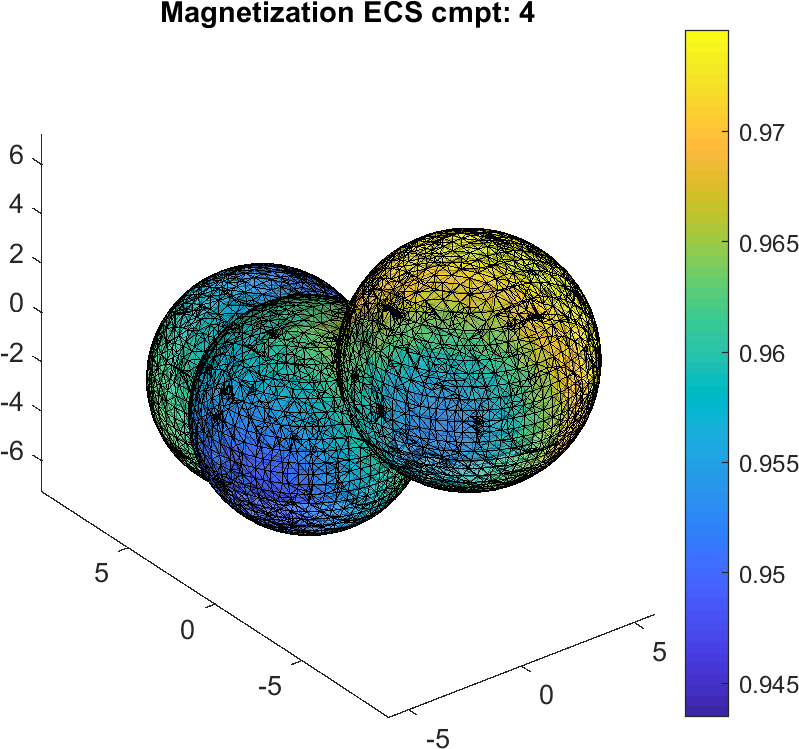
\includegraphics[width=0.35\textwidth]{plot_magnetization/3sph_ecs_perm.png} \\
    \vspace{0.8cm}
    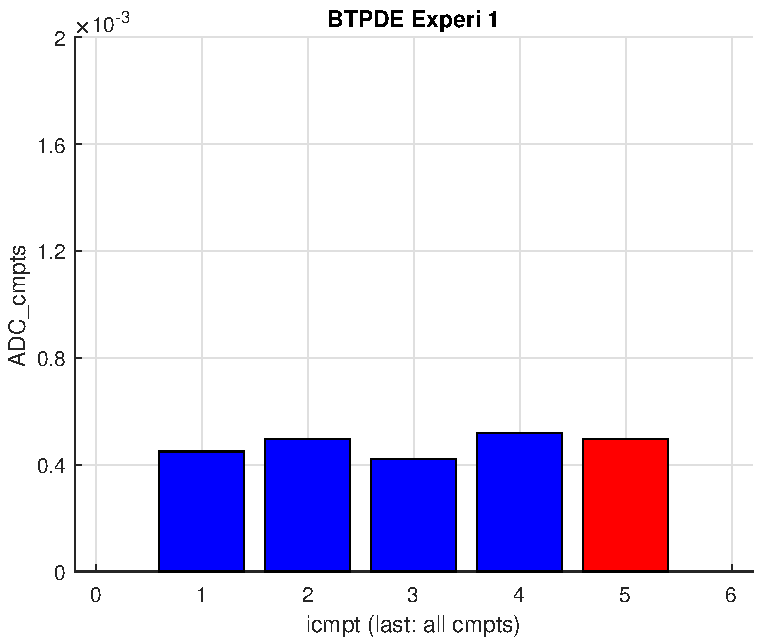
\includegraphics[width=0.35\textwidth]{plot_adc/btpde_3sph_perm.pdf} \quad
    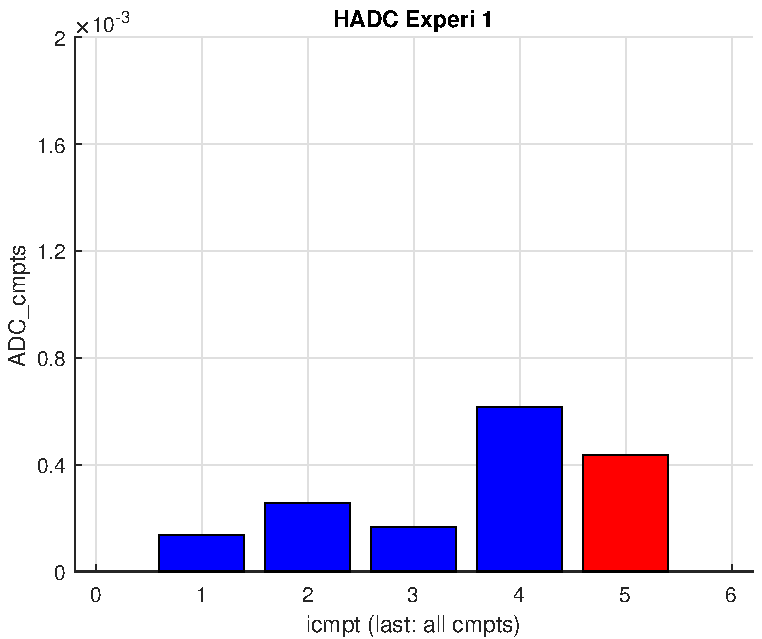
\includegraphics[width=0.35\textwidth]{plot_adc/hadc_3sph_perm.pdf}
    \caption{Geometry: 3 spheres, tight wrap ECS, ecs\_gap = 0.3, $\vec{u}_{\vec{g}}=(1,1,0)^\transpose / \sqrt{2}$, $\sigma^\text{in}=\sigma^{ecs}=2\times10^{-3}\dunit$, $\kappa=1\e{-3} \kunit$ (left), $\kappa = 0\kunit$ (right). PGSE ($\delta=5\tunit,\Delta=5\tunit$). The vertical bars indicate the ADC in each compartment. The ADC in the rightmost position is the ADC that takes into account the diffusion in all the compartments.}
    \label{fig:perm}
\end{figure}





\subsection{Myelin layer}

In Fig. \ref{fig:myelin} we show the diffusion in cylindrical cells, the myelin layer, and the ECS. The ADC is higher in the myelin layer than in the cells, because for spins in the myelin layer diffusion occurs in the tangential direction (around the circle). At longer diffusion times, the ADC of both the myelin layer and the cells becomes very low. The ADC is the highest in the ECS, because the diffusion distance can be longer than the diameter of a cell, since the diffusing spins can move around multiple cells.

\begin{figure}
    \centering
    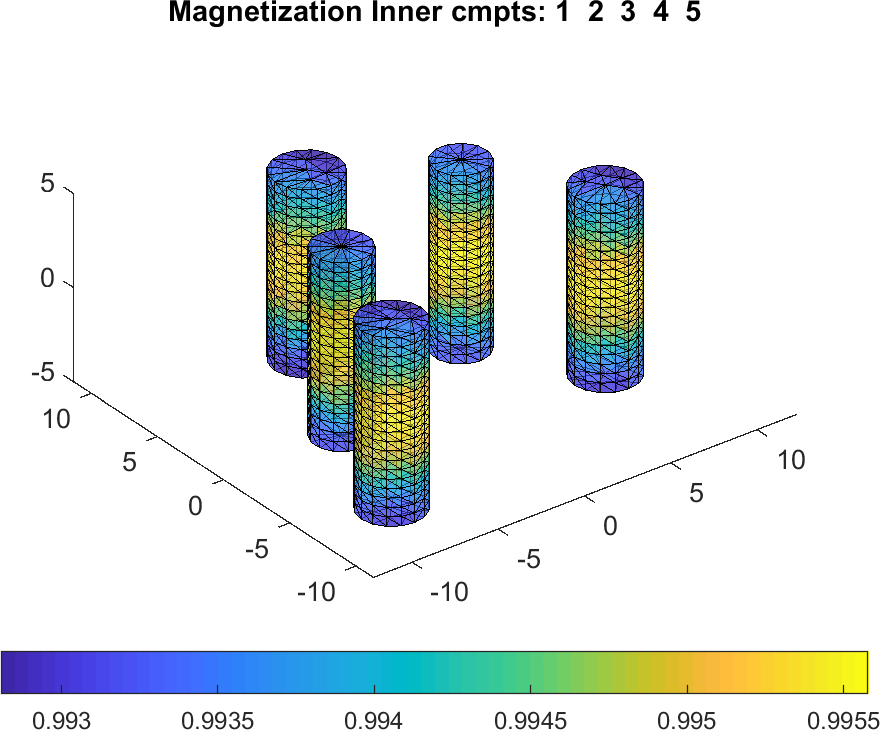
\includegraphics[width=0.35\textwidth]{plot_magnetization/5cyl_cells_myelin.png}\quad
    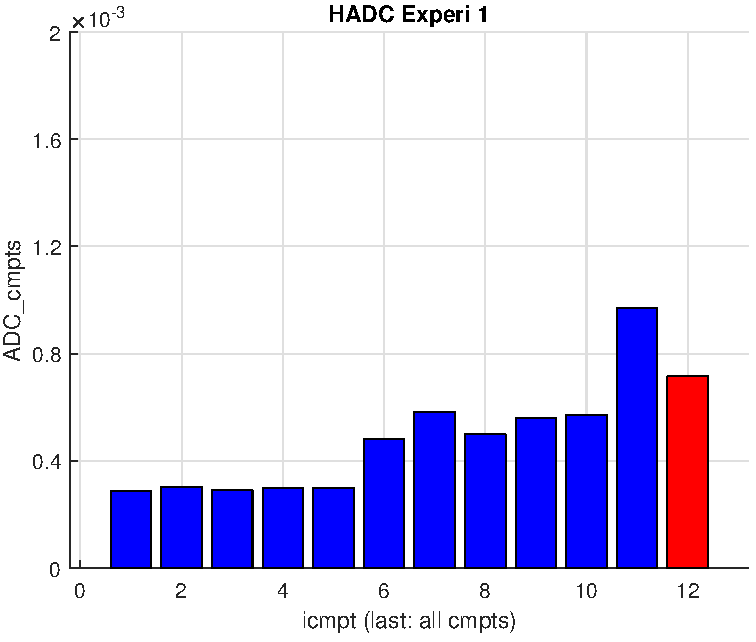
\includegraphics[width=0.35\textwidth]{plot_adc/hadc_5cyl1.pdf}\\
    \vspace{0.2cm}
    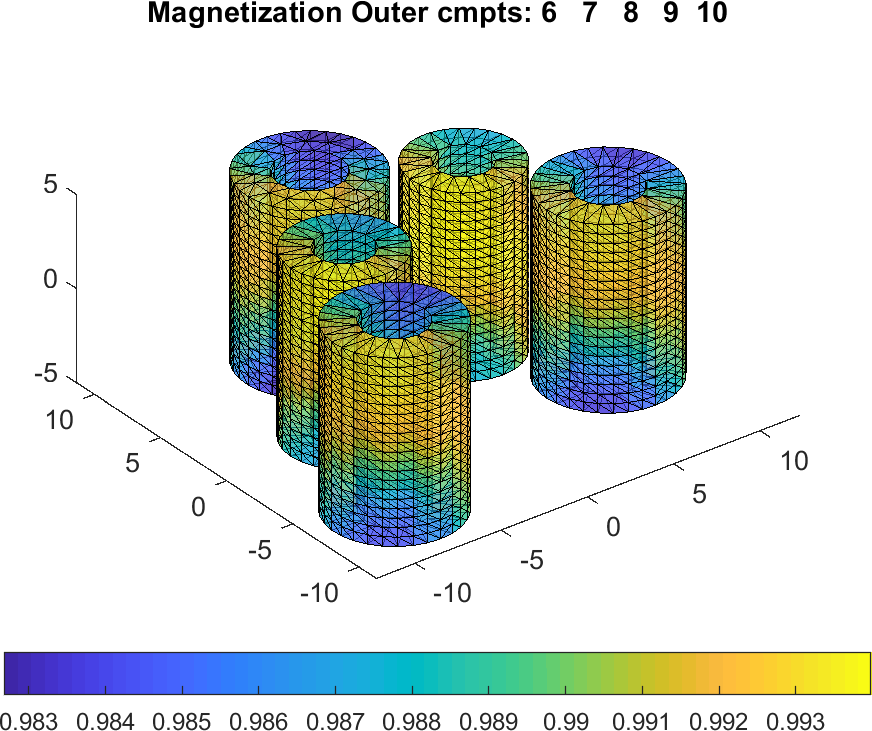
\includegraphics[width=0.35\textwidth]{plot_magnetization/5cyl_myelin_myelin.png} \quad
    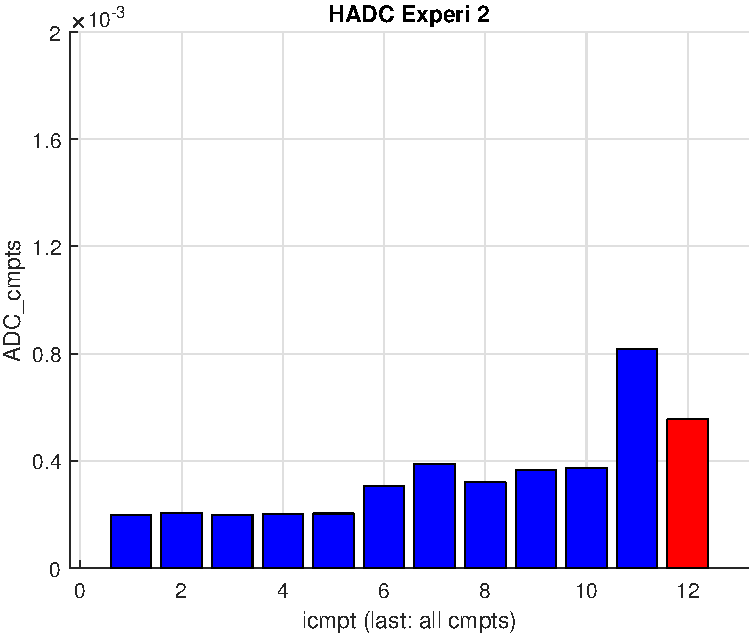
\includegraphics[width=0.35\textwidth]{plot_adc/hadc_5cyl2.pdf}\\
    \vspace{0.2cm}
    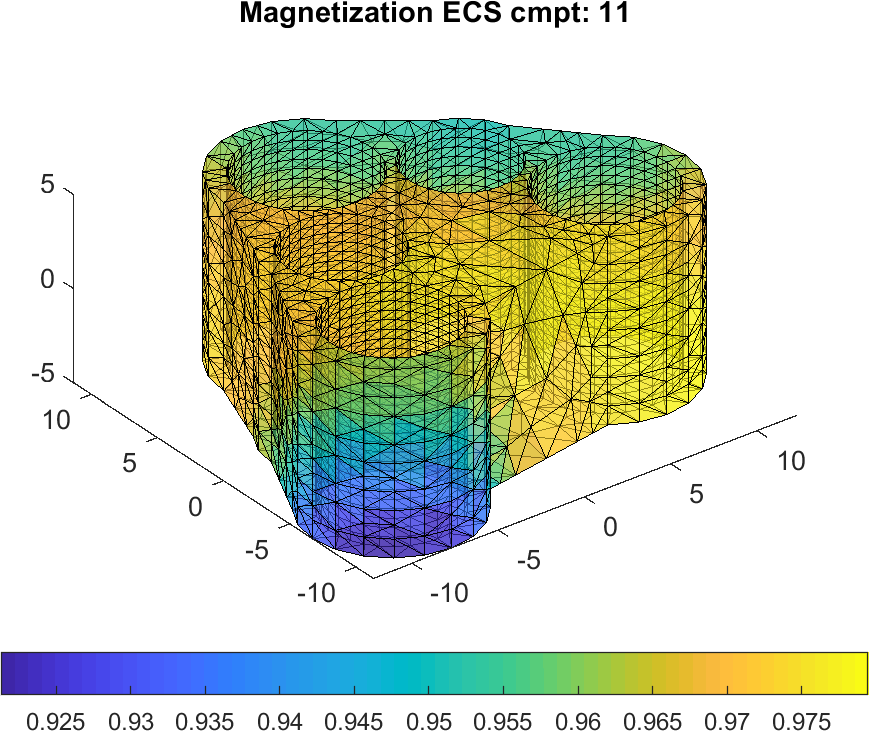
\includegraphics[width=0.35\textwidth]{plot_magnetization/5cyl_ecs_myelin.png} \quad
    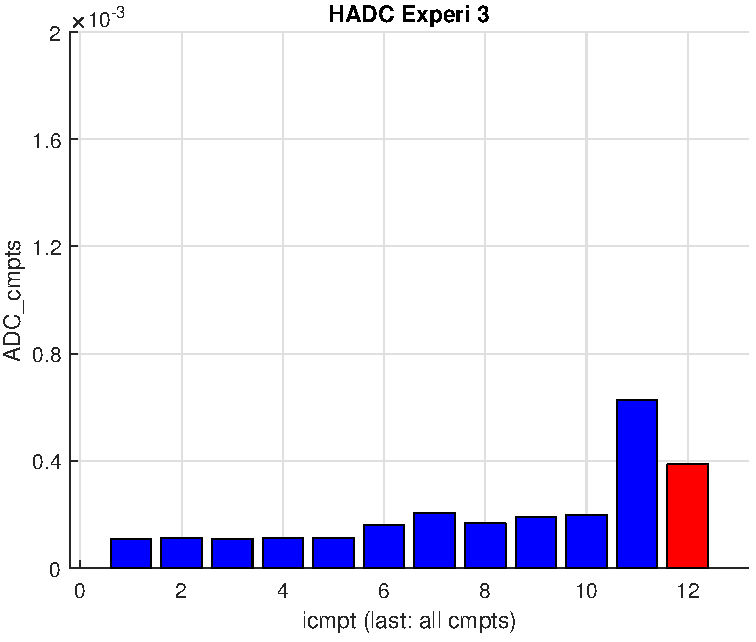
\includegraphics[width=0.35\textwidth]{plot_adc/hadc_5cyl3.pdf}
    \caption{Geometry: 5 cylinders, myelin layer, $r_\text{in}/r_\text{out}=0.5$, tight wrap ECS, ecs\_gap = 0.3, $\kappa=0\kunit$, $\vec{u}_{\vec{g}} = (1,1,1)^\transpose / \sqrt{3}$, $\sigma^\text{in}=\sigma^\text{out}=\sigma^\text{ecs}=2\times10^{-3}\dunit$, 3 experiments: PGSE ($\delta=5\tunit,\Delta=5,10,20\tunit$). Left: the magnetization at $\Delta=5\tunit$. Right: the ADC values. The vertical bars indicate the ADC in each compartment. The ADC in the rightmost position is the ADC that takes into account the diffusion in all the compartments.}
    \label{fig:myelin}
\end{figure}





\subsection{Twisting and bending}

In Fig. \ref{fig:bend_twist} we show the effect of bending and twising in cylindrical cells in multiple gradient directions. The HADC is obtained in 20 directions uniformly distributed in the sphere. We used spherical harmonics interpolation to interpolate the HADC in the entire sphere. Then we deformed the radius of the unit sphere to be proportional to the interpolated HADC and plotted the 3D shape. The color axis also indicates the value of the interpolated HADC.

\begin{figure}[!ht]
    \centering
    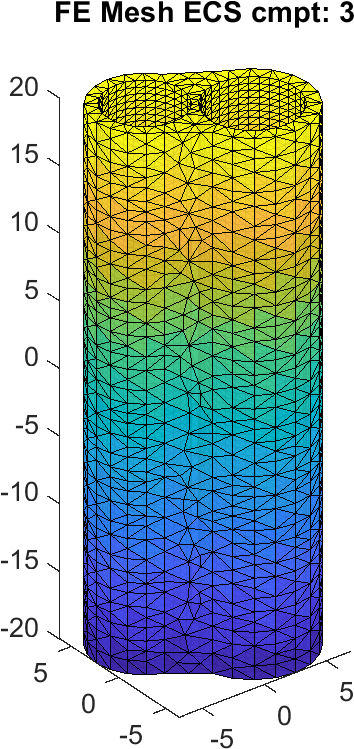
\includegraphics[width=0.2448\textwidth]{plot_femesh/2cyl_ecs_canonical.png} \quad\quad
    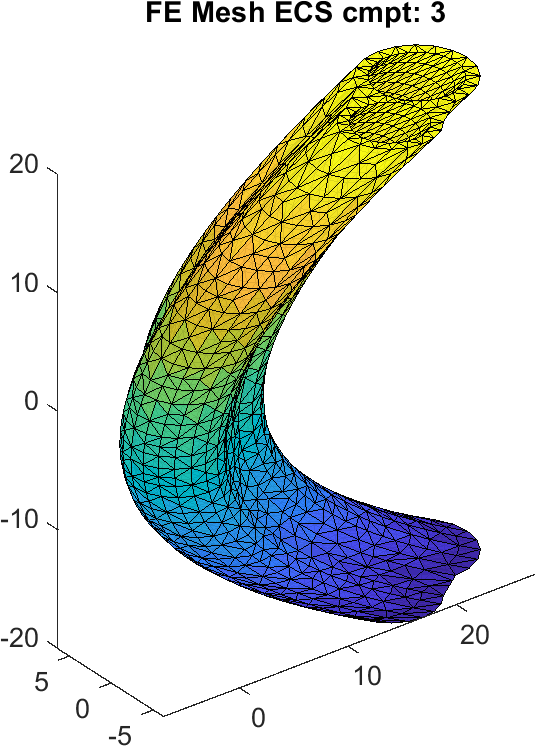
\includegraphics[width=0.37\textwidth]{plot_femesh/2cyl_ecs_bend.png} \quad\quad
    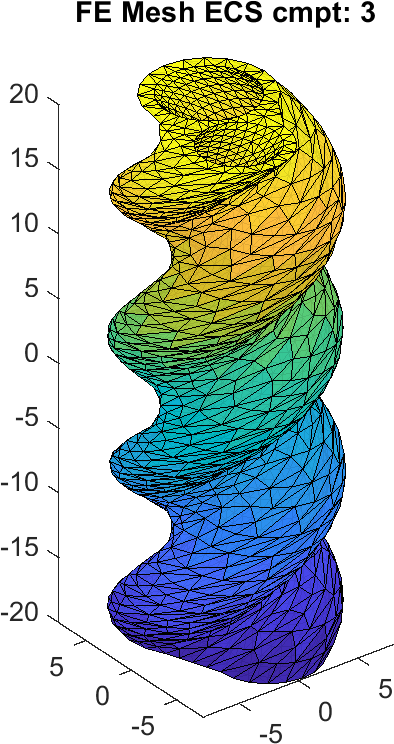
\includegraphics[width=0.2725\textwidth]{plot_femesh/2cyl_ecs_twist.png} \\
    \vspace{0.5cm}
    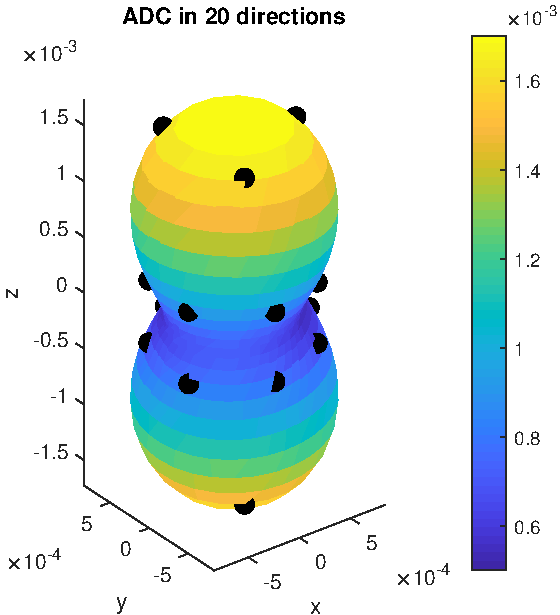
\includegraphics[width=0.2874\textwidth]{adc_alldir/none.pdf}
    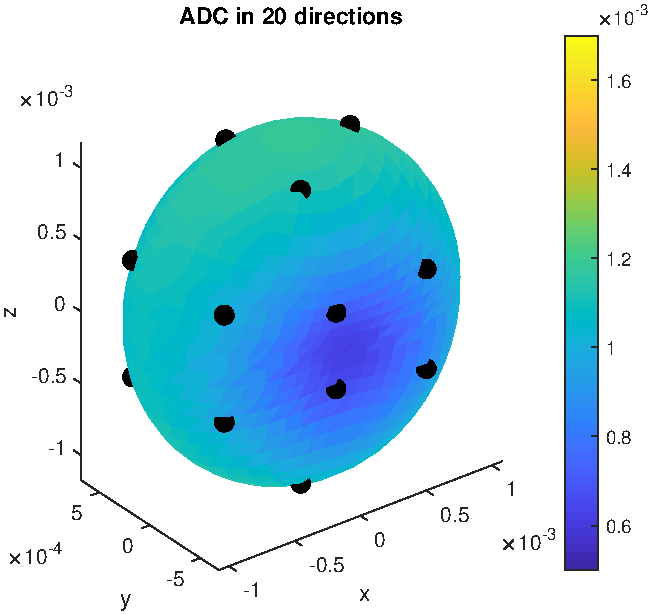
\includegraphics[width=0.3358\textwidth]{adc_alldir/bend.pdf}
    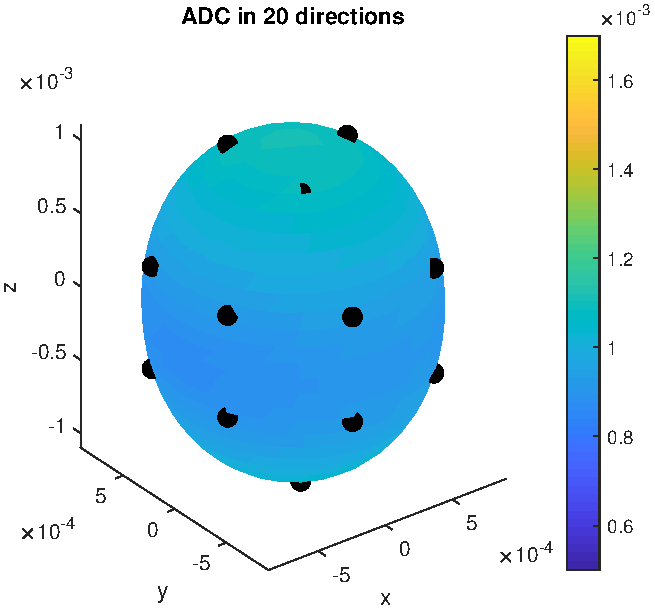
\includegraphics[width=0.3368\textwidth]{adc_alldir/twist.pdf}
    \caption{Geometry: 2 cylinders, no myelin layer, tight wrap ECS, ecs\_gap = 0.3, $\kappa=0\kunit$, $\sigma^\text{out}=\sigma^\text{ecs}=2\times10^{-3}\dunit$, PGSE ($\delta=2.5\tunit,\Delta=5\tunit$). Left: canonical configuration. Middle: bend parameter = 0.05. Right: twist parameter = 0.30. Top: FE mesh of the ECS (the FE mesh of the axon compartments numbered 1 and 2 not shown). Bottom: interpolated values of the HADC on the unit sphere, and then the sphere was distorted to reflect the value of the HADC. The color axis also gives the value of the HADC in the various gradient directions. The black dots indicate the 20 original gradient-directions in which the HADC was simulated. The spherical harmonics interpolation takes the 20 original directions into 900 directions uniformly distributed on the sphere.}
    \label{fig:bend_twist}
\end{figure}




\subsection{Neuron examples}

In Figures \ref{fig:spindle}, \ref{fig:signal_neuronmodule}, and \ref{fig:sig_hardi_neuron} we display figures from the functions plot\_femesh, plot\_field, plot\_signal, plot\_hardi. The geometrical configuration is the spindle neuron {\it 03b\_spindle6aFI}. The intrinsic diffusion coefficient is set to $\Dintr = 2\times 10^{-3} \dunit$, with nonpermeable membrane. We simulated 2 diffusion-encoding sequences:
\begin{enumerate}
    \item $f_1$ is PGSE ($\delta=10.6\tunit$, $\Delta=13\tunit$);
    \item $f_2$ is PGSE ($\delta=10.6\tunit$, $\Delta=73\tunit$).
\end{enumerate}

\begin{figure}
    \centering
    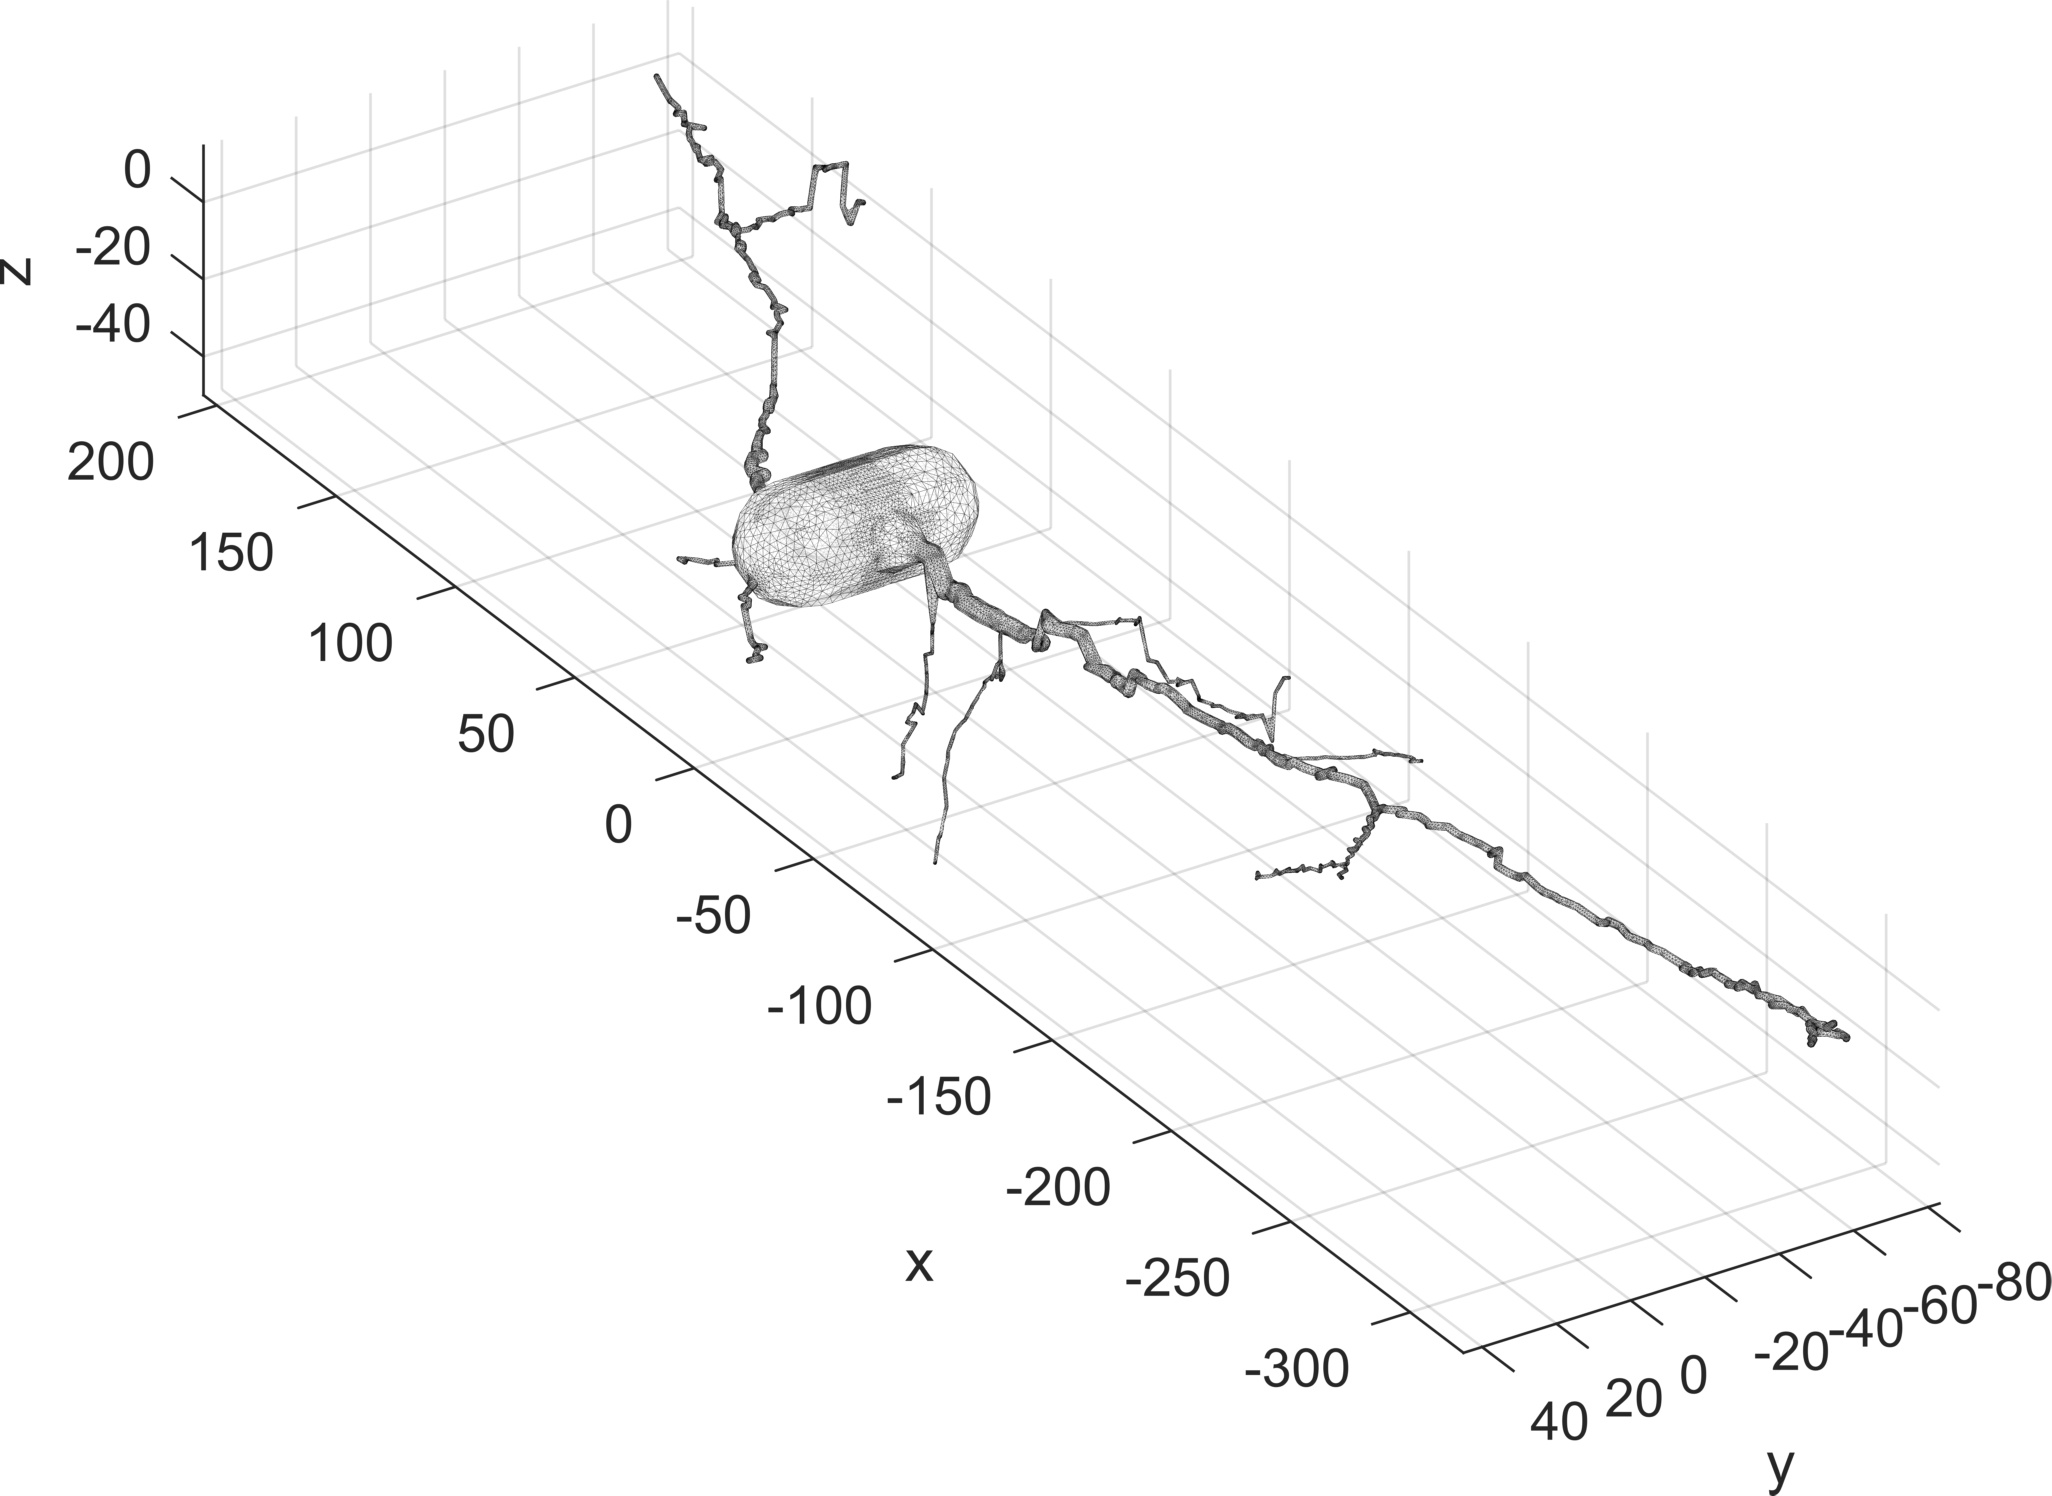
\includegraphics[width=0.49\textwidth]{paper_neuron/03a_spindle6aFI_FEmesh.jpg}
    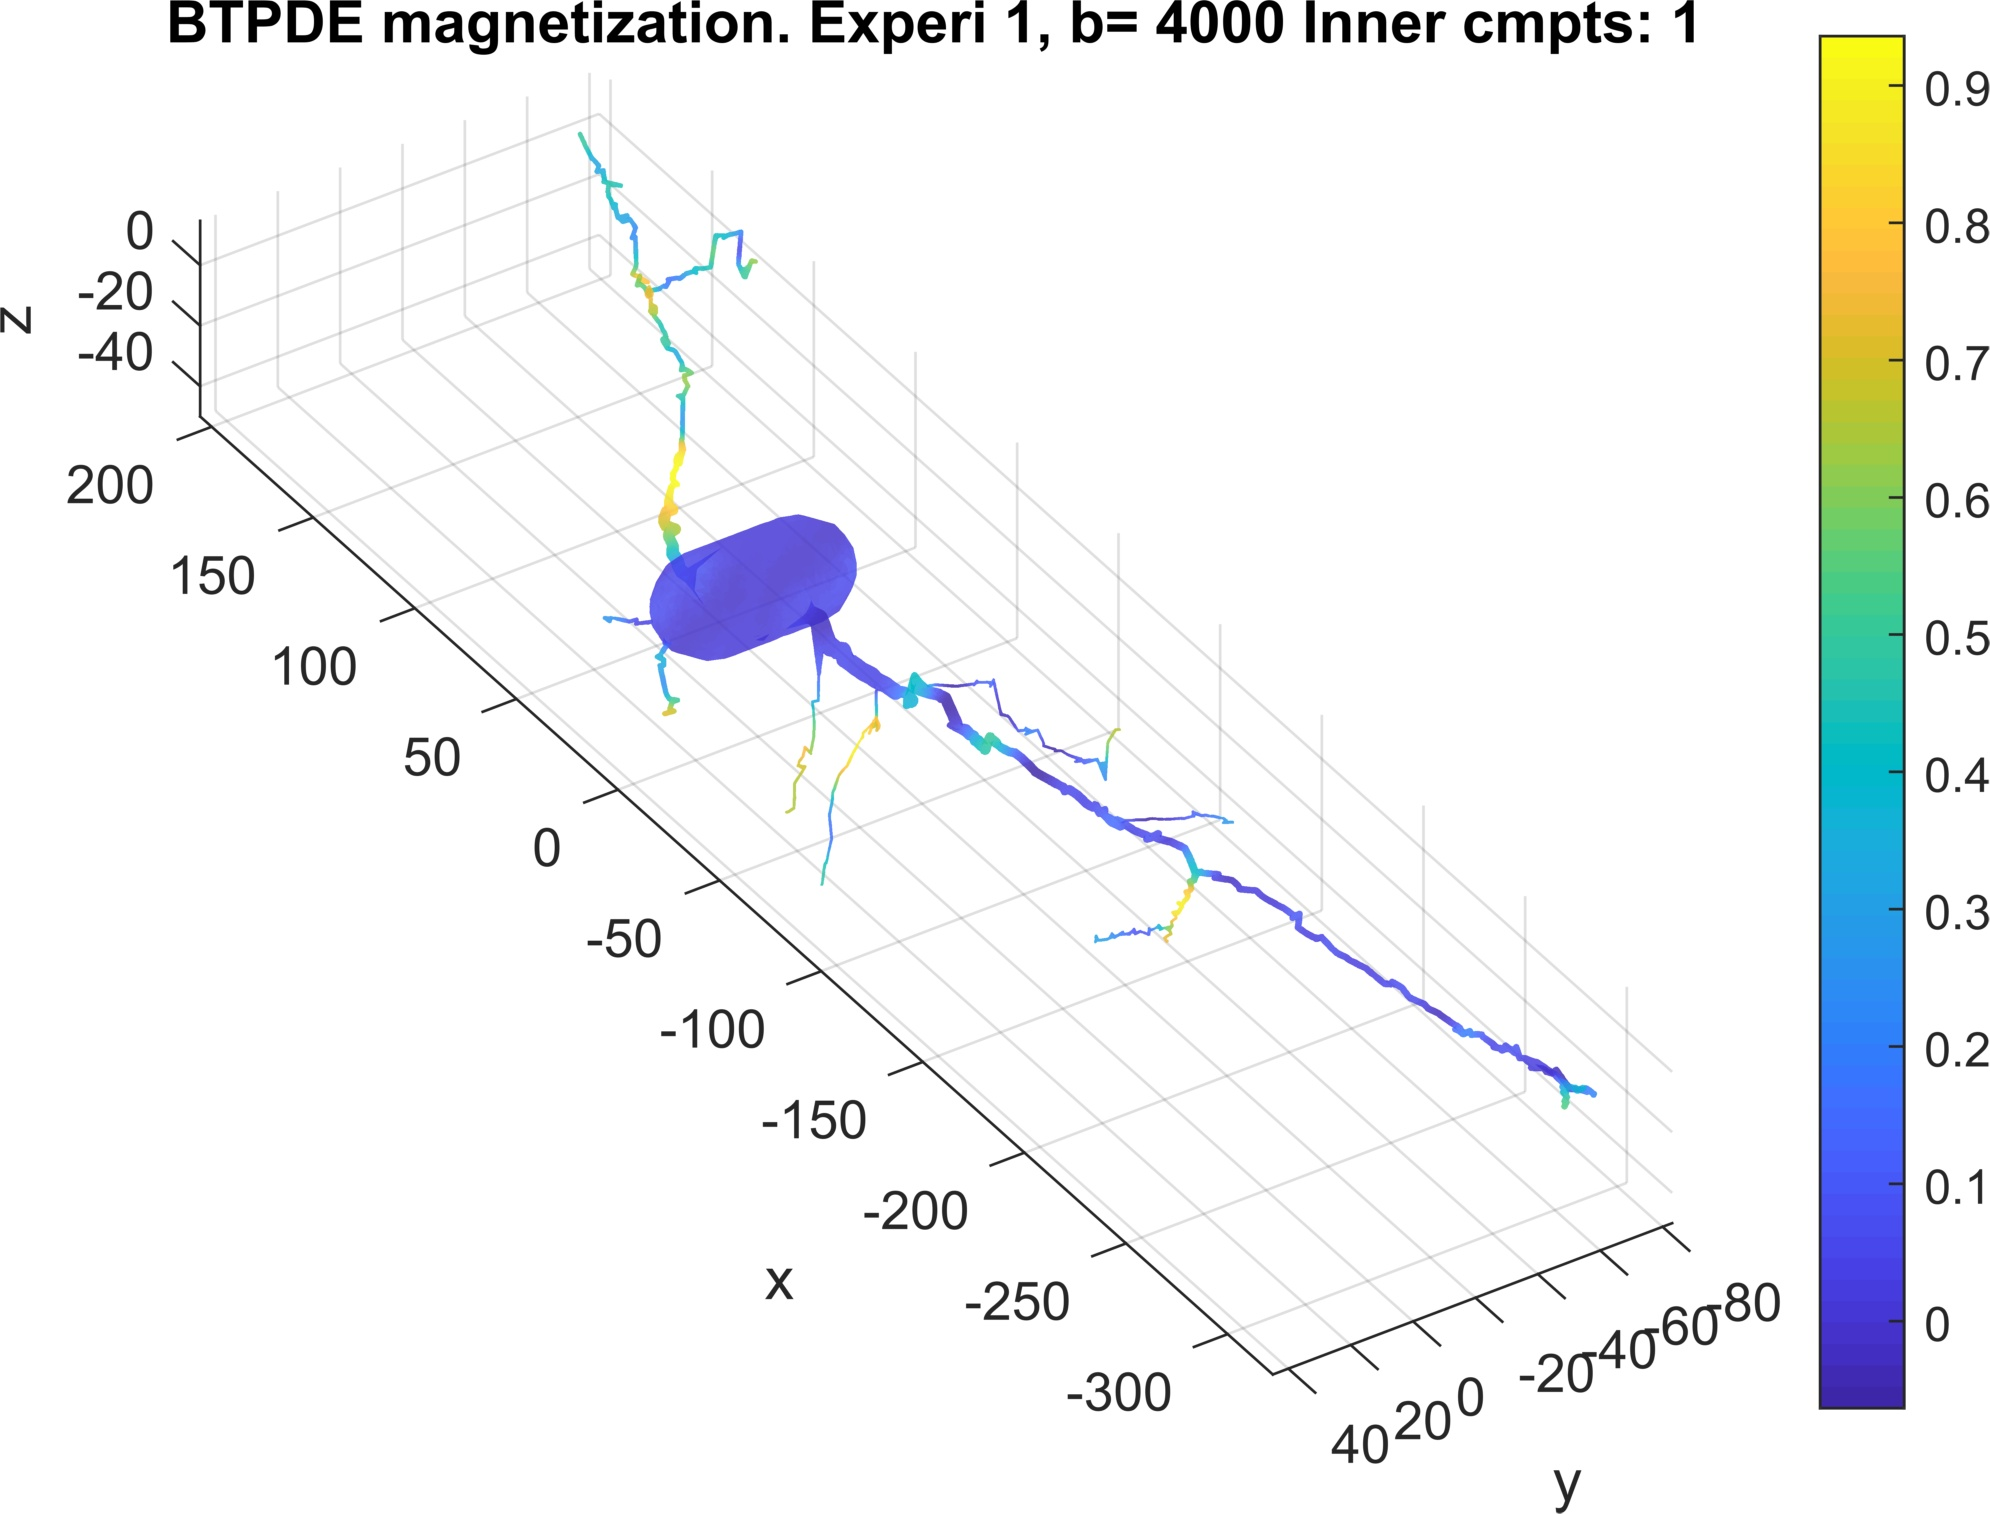
\includegraphics[width=0.49\textwidth]{paper_neuron/03a_spindle6aFI_PDESOLUTION.jpg}
    \caption{Left: The finite elements mesh of the neuron {\it 03b\_spindle6aFI} (using the command plot\_femesh). The unit is \lunit. Right: The PDE solution (magnetization) on the neuron {\it 03b\_spindle6aFI} in the diffusion-encoding direction (1, 1, 1) (using the command plot\_field). The diffusion-encoding sequence is PGSE ($\delta=10.6\tunit$, $\Delta=13\tunit$). The b-value is $b=4000\bunit$.}
    \label{fig:spindle}
\end{figure}

\begin{figure}
    \centering
    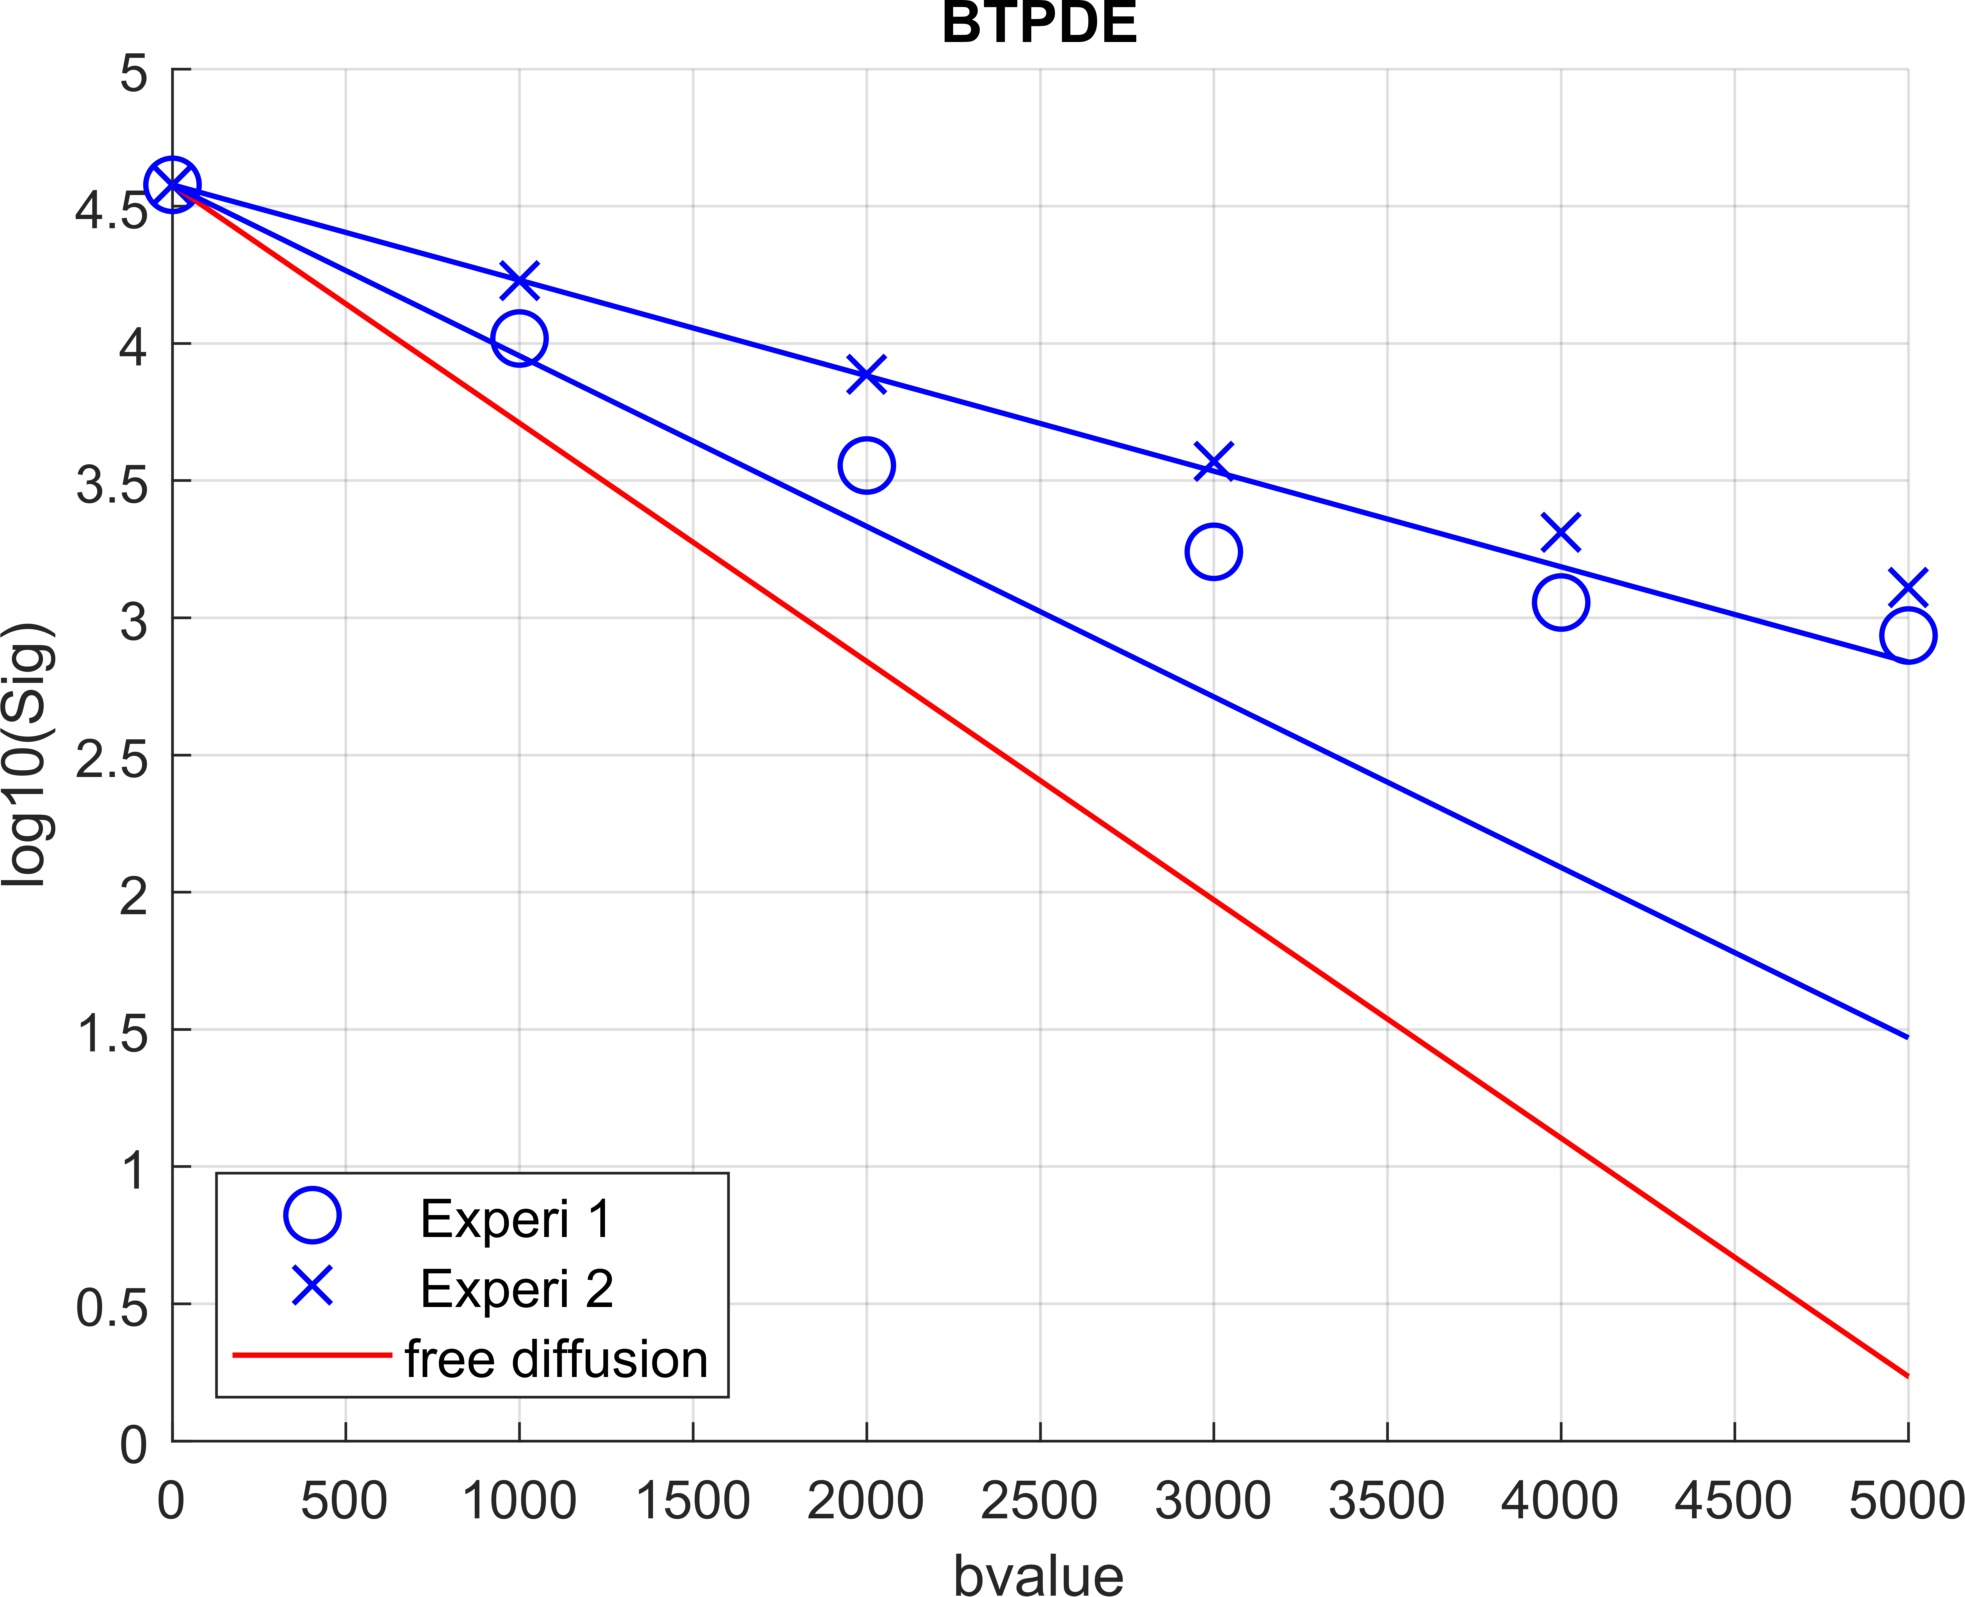
\includegraphics[width=0.4\textwidth]{paper_neuron/03a_spindle6aFI_PLOTSIGNAL.jpg}
    \caption{The (non-normalized) simulated signal of the neuron {\it 03b\_spindle6aFI} in the diffusion-encoding direction (1, 1, 1) (using the command plot\_signal). For Experiment 1, the diffusion-encoding sequence is PGSE ($\delta=10.6\tunit$, $\Delta=13\tunit$). For Experiment 2, the diffusion-encoding sequence is PGSE ($\delta=10.6\tunit$, $\Delta=73\tunit$).}
    \label{fig:signal_neuronmodule}
\end{figure}

\begin{figure}
    \centering
    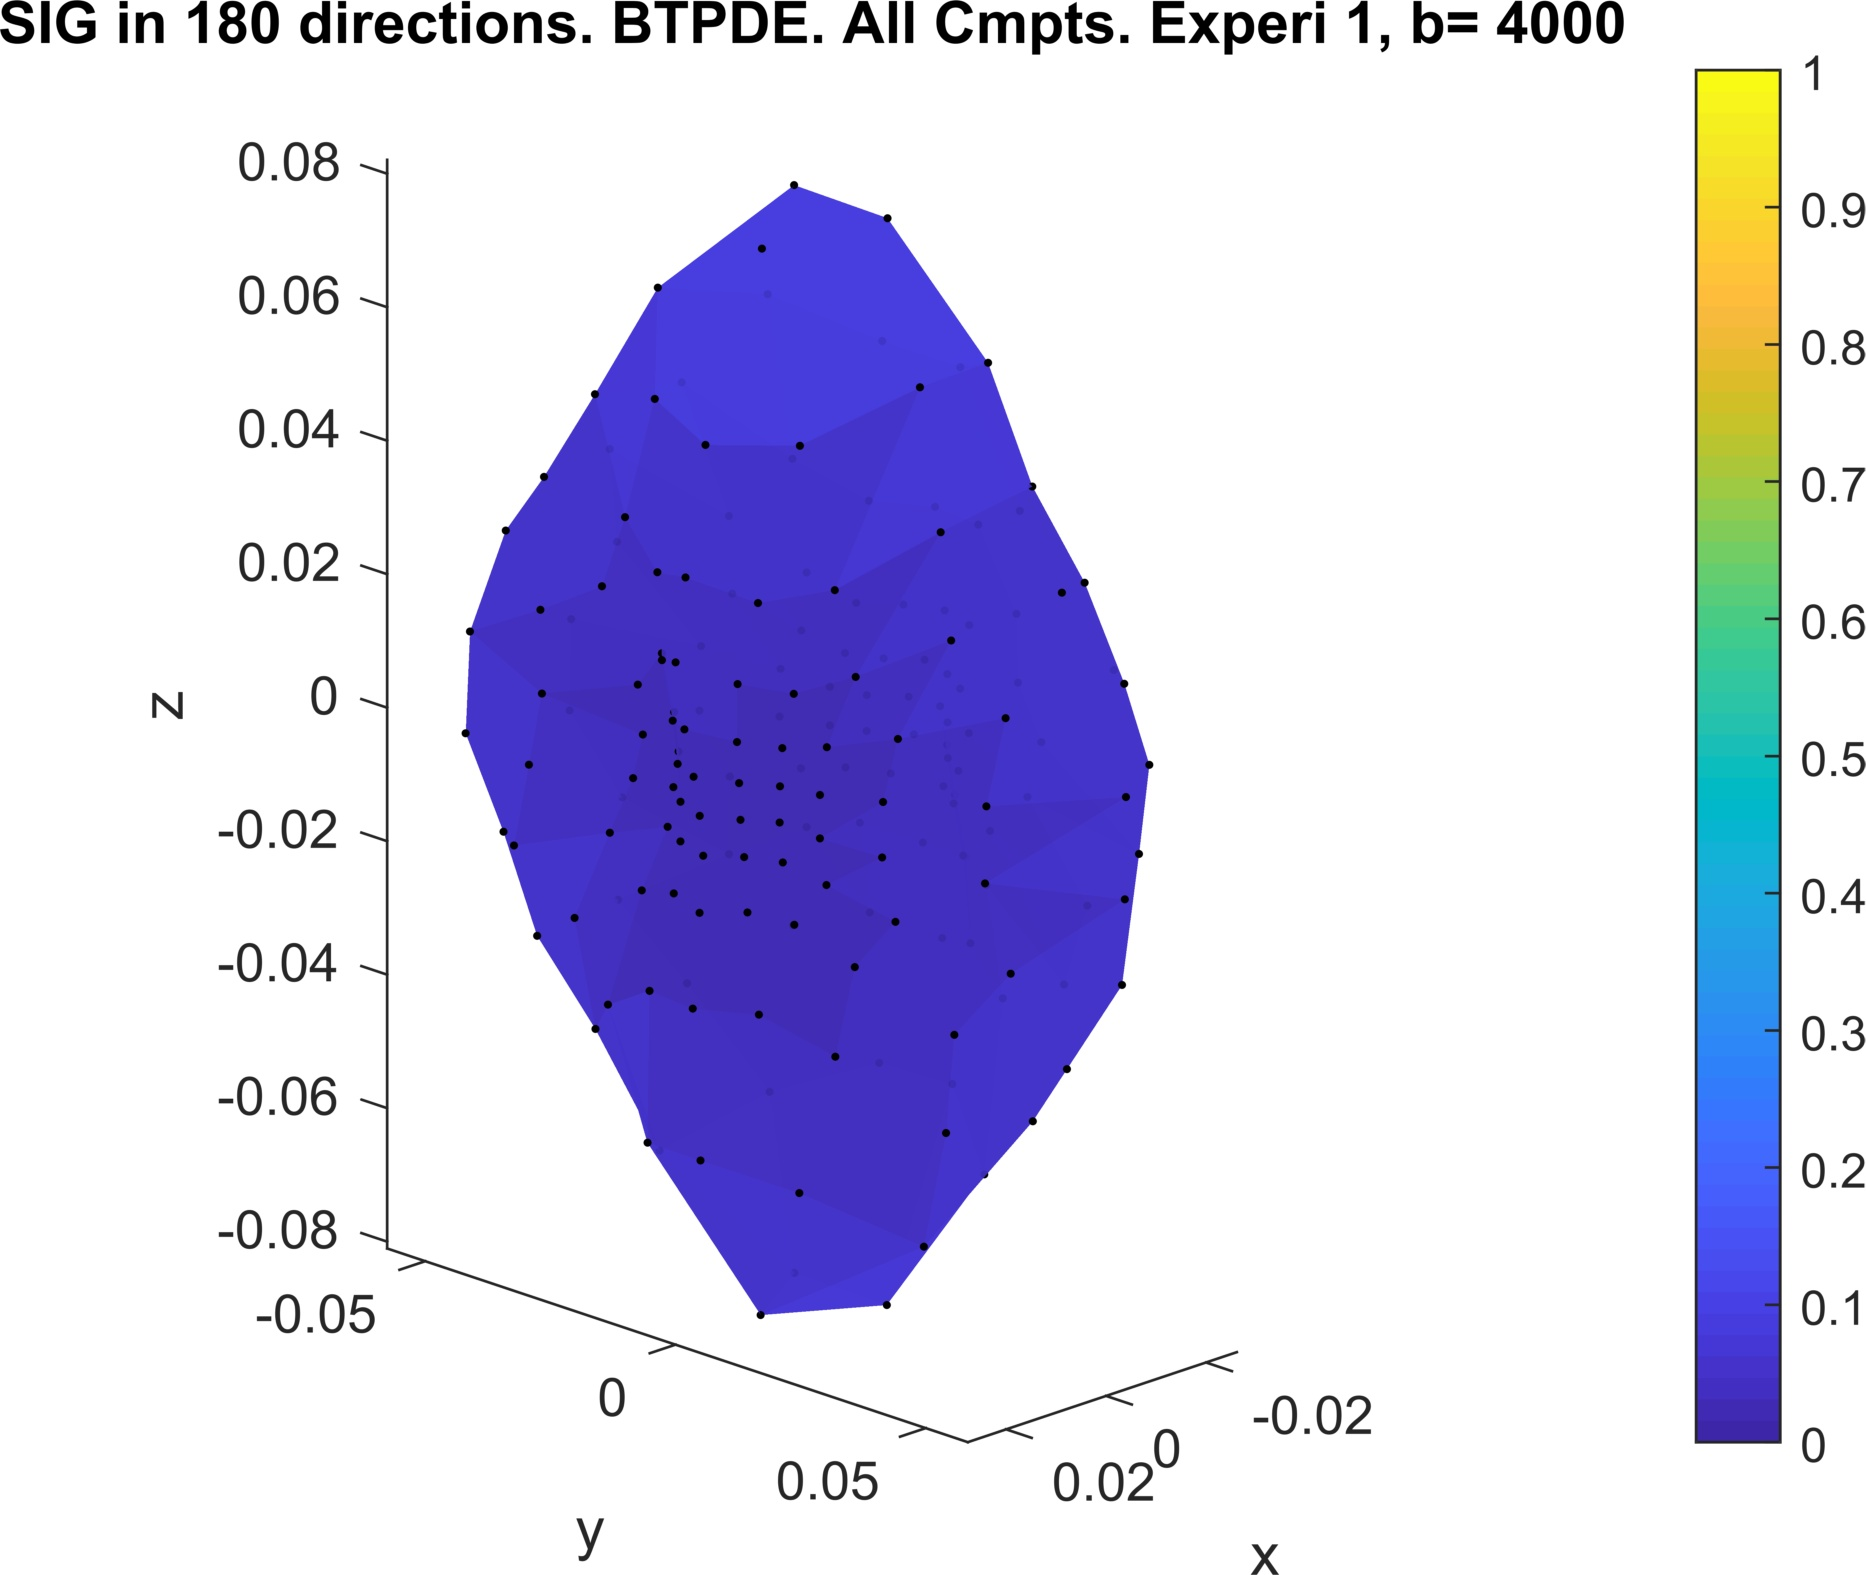
\includegraphics[width=0.45\textwidth]{paper_neuron/03a_spindle6aFI_exp1b4000.jpg}
    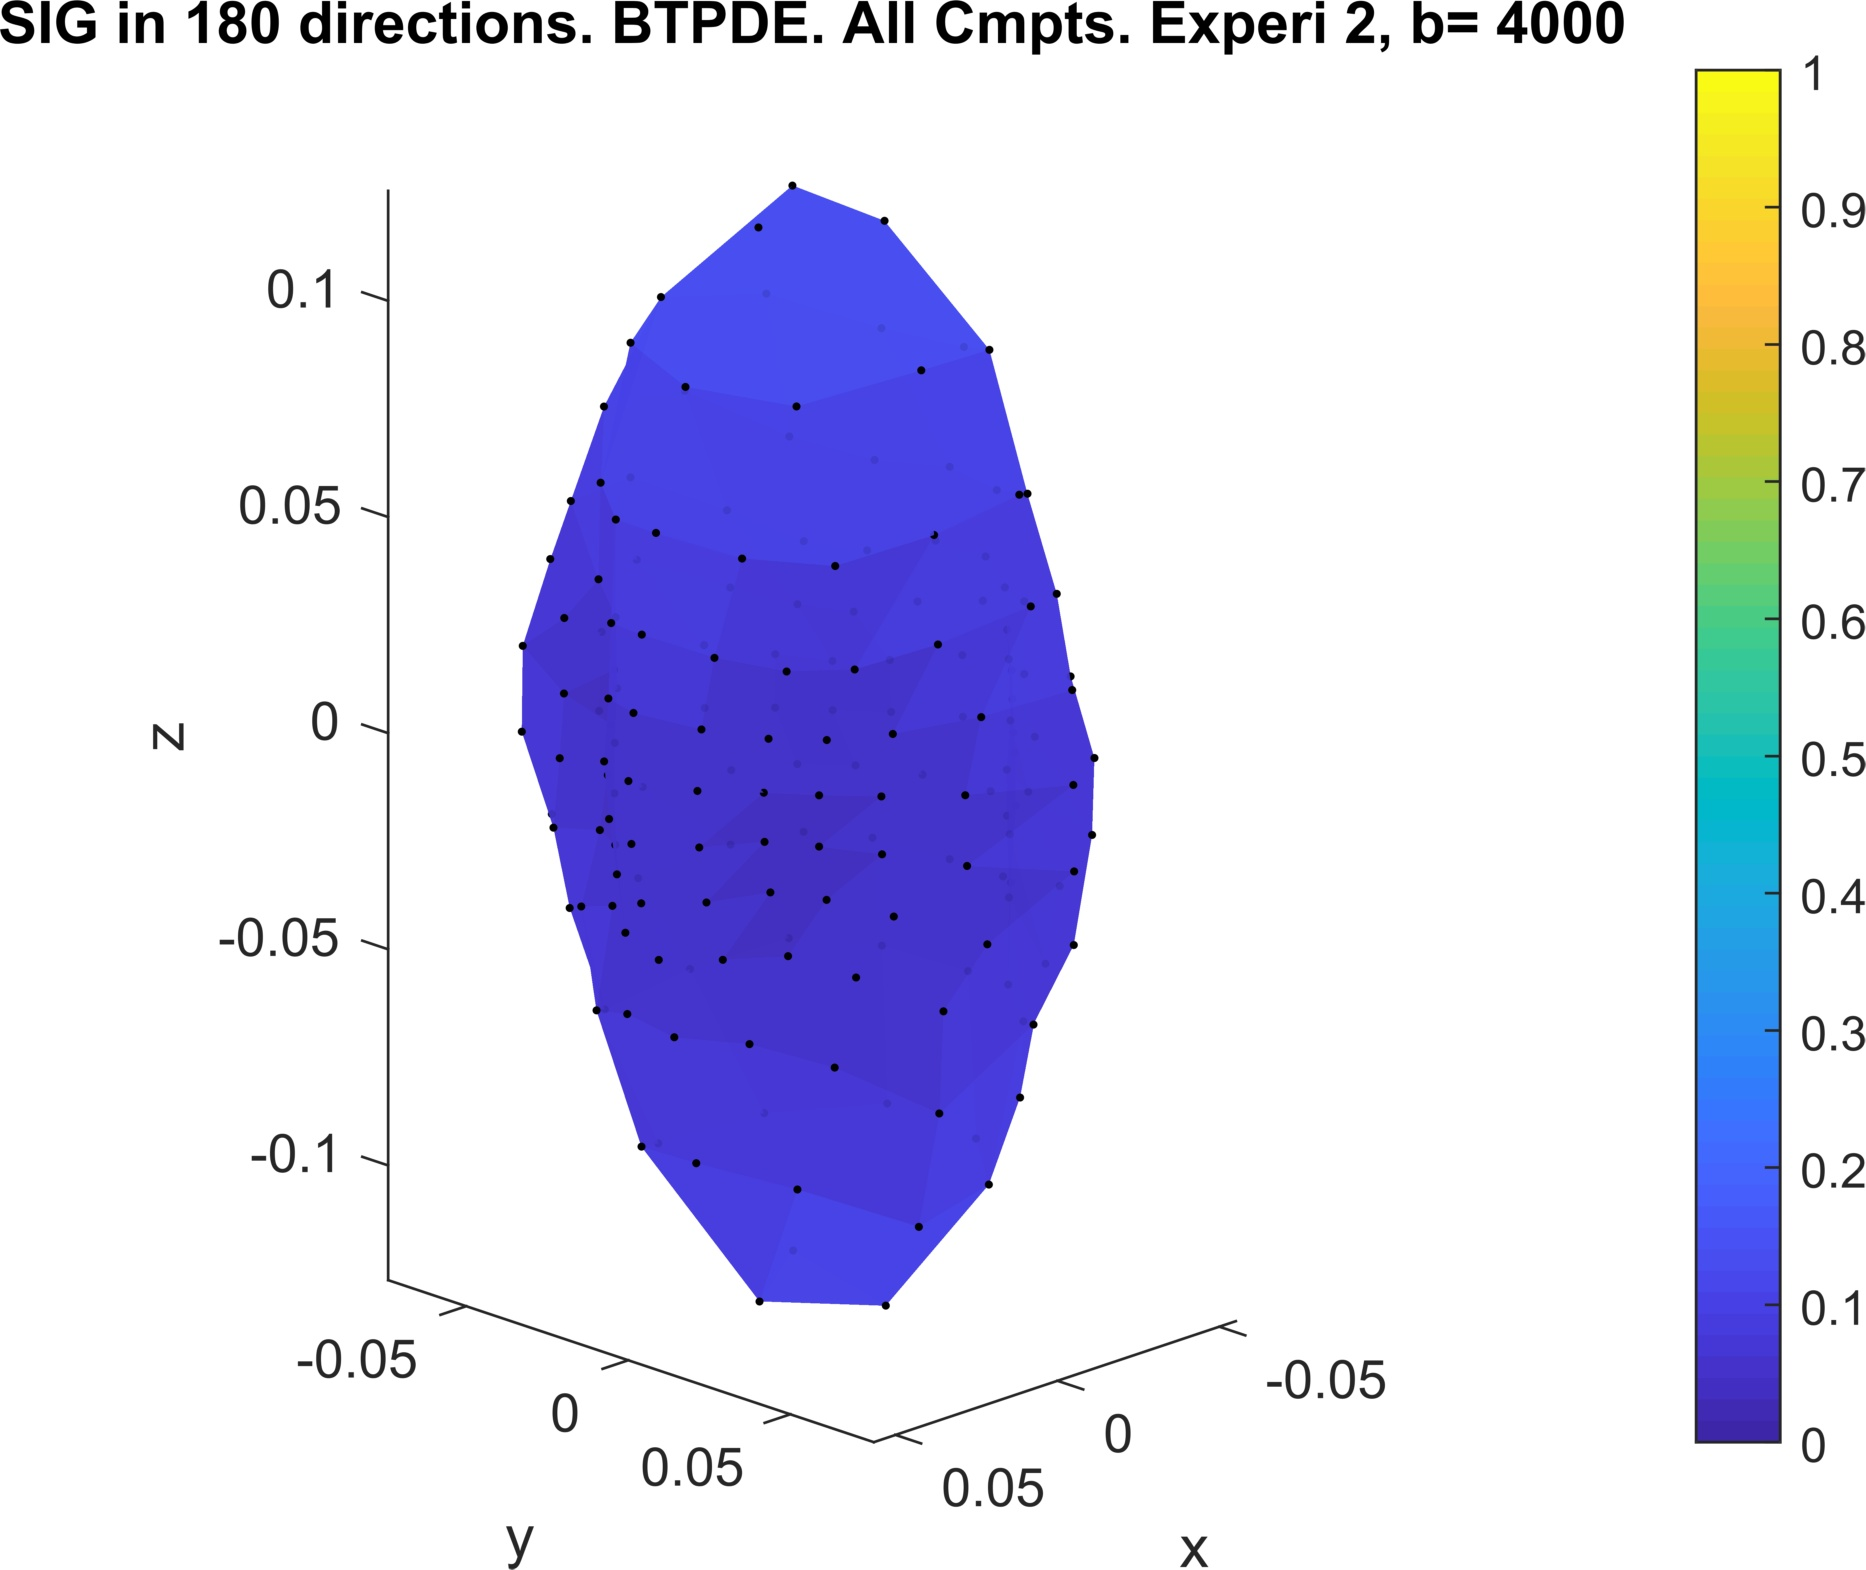
\includegraphics[width=0.45\textwidth]{paper_neuron/03a_spindle6aFI_exp2b4000.jpg}
    \caption{The simulated signal in 180 diffusion-encoding directions for the neuron {\it 03b\_spindle6aFI} (using the command plot\_hardi). Left: The signal in 180 directions with PGSE ($\delta=10.6\tunit$, $\Delta=13\tunit$) and $b=4000\bunit$. Right: The signal in 180 directions with PGSE ($\delta=10.6\tunit$, $\Delta=73\tunit$) and $b=4000\bunit$.}
    \label{fig:sig_hardi_neuron}
\end{figure}



\subsection{Matrix Formalism examples}

Below we display some example outputs from the Matrix Formalism Module. The geometrical configuration is one dendrite branch of a spindle neuron, {\it 03b\_spindle6aACC\_dendrites\_2}, shown in Figure \ref{fig:spindle_dendrite_eigfunc}. The intrinsic diffusion coefficient is set to $\Dintr = 2\times 10^{-3} \dunit$, with an impermeable membrane. We simulated 2 diffusion-encoding sequences:
\begin{enumerate}
    \item $f_1$ is PGSE ($\delta=10.6\tunit$, $\Delta=13\tunit$),
    \item $f_2$ is PGSE ($\delta=10.6\tunit$, $\Delta=73\tunit$).
\end{enumerate}

\begin{figure}
    \centering
    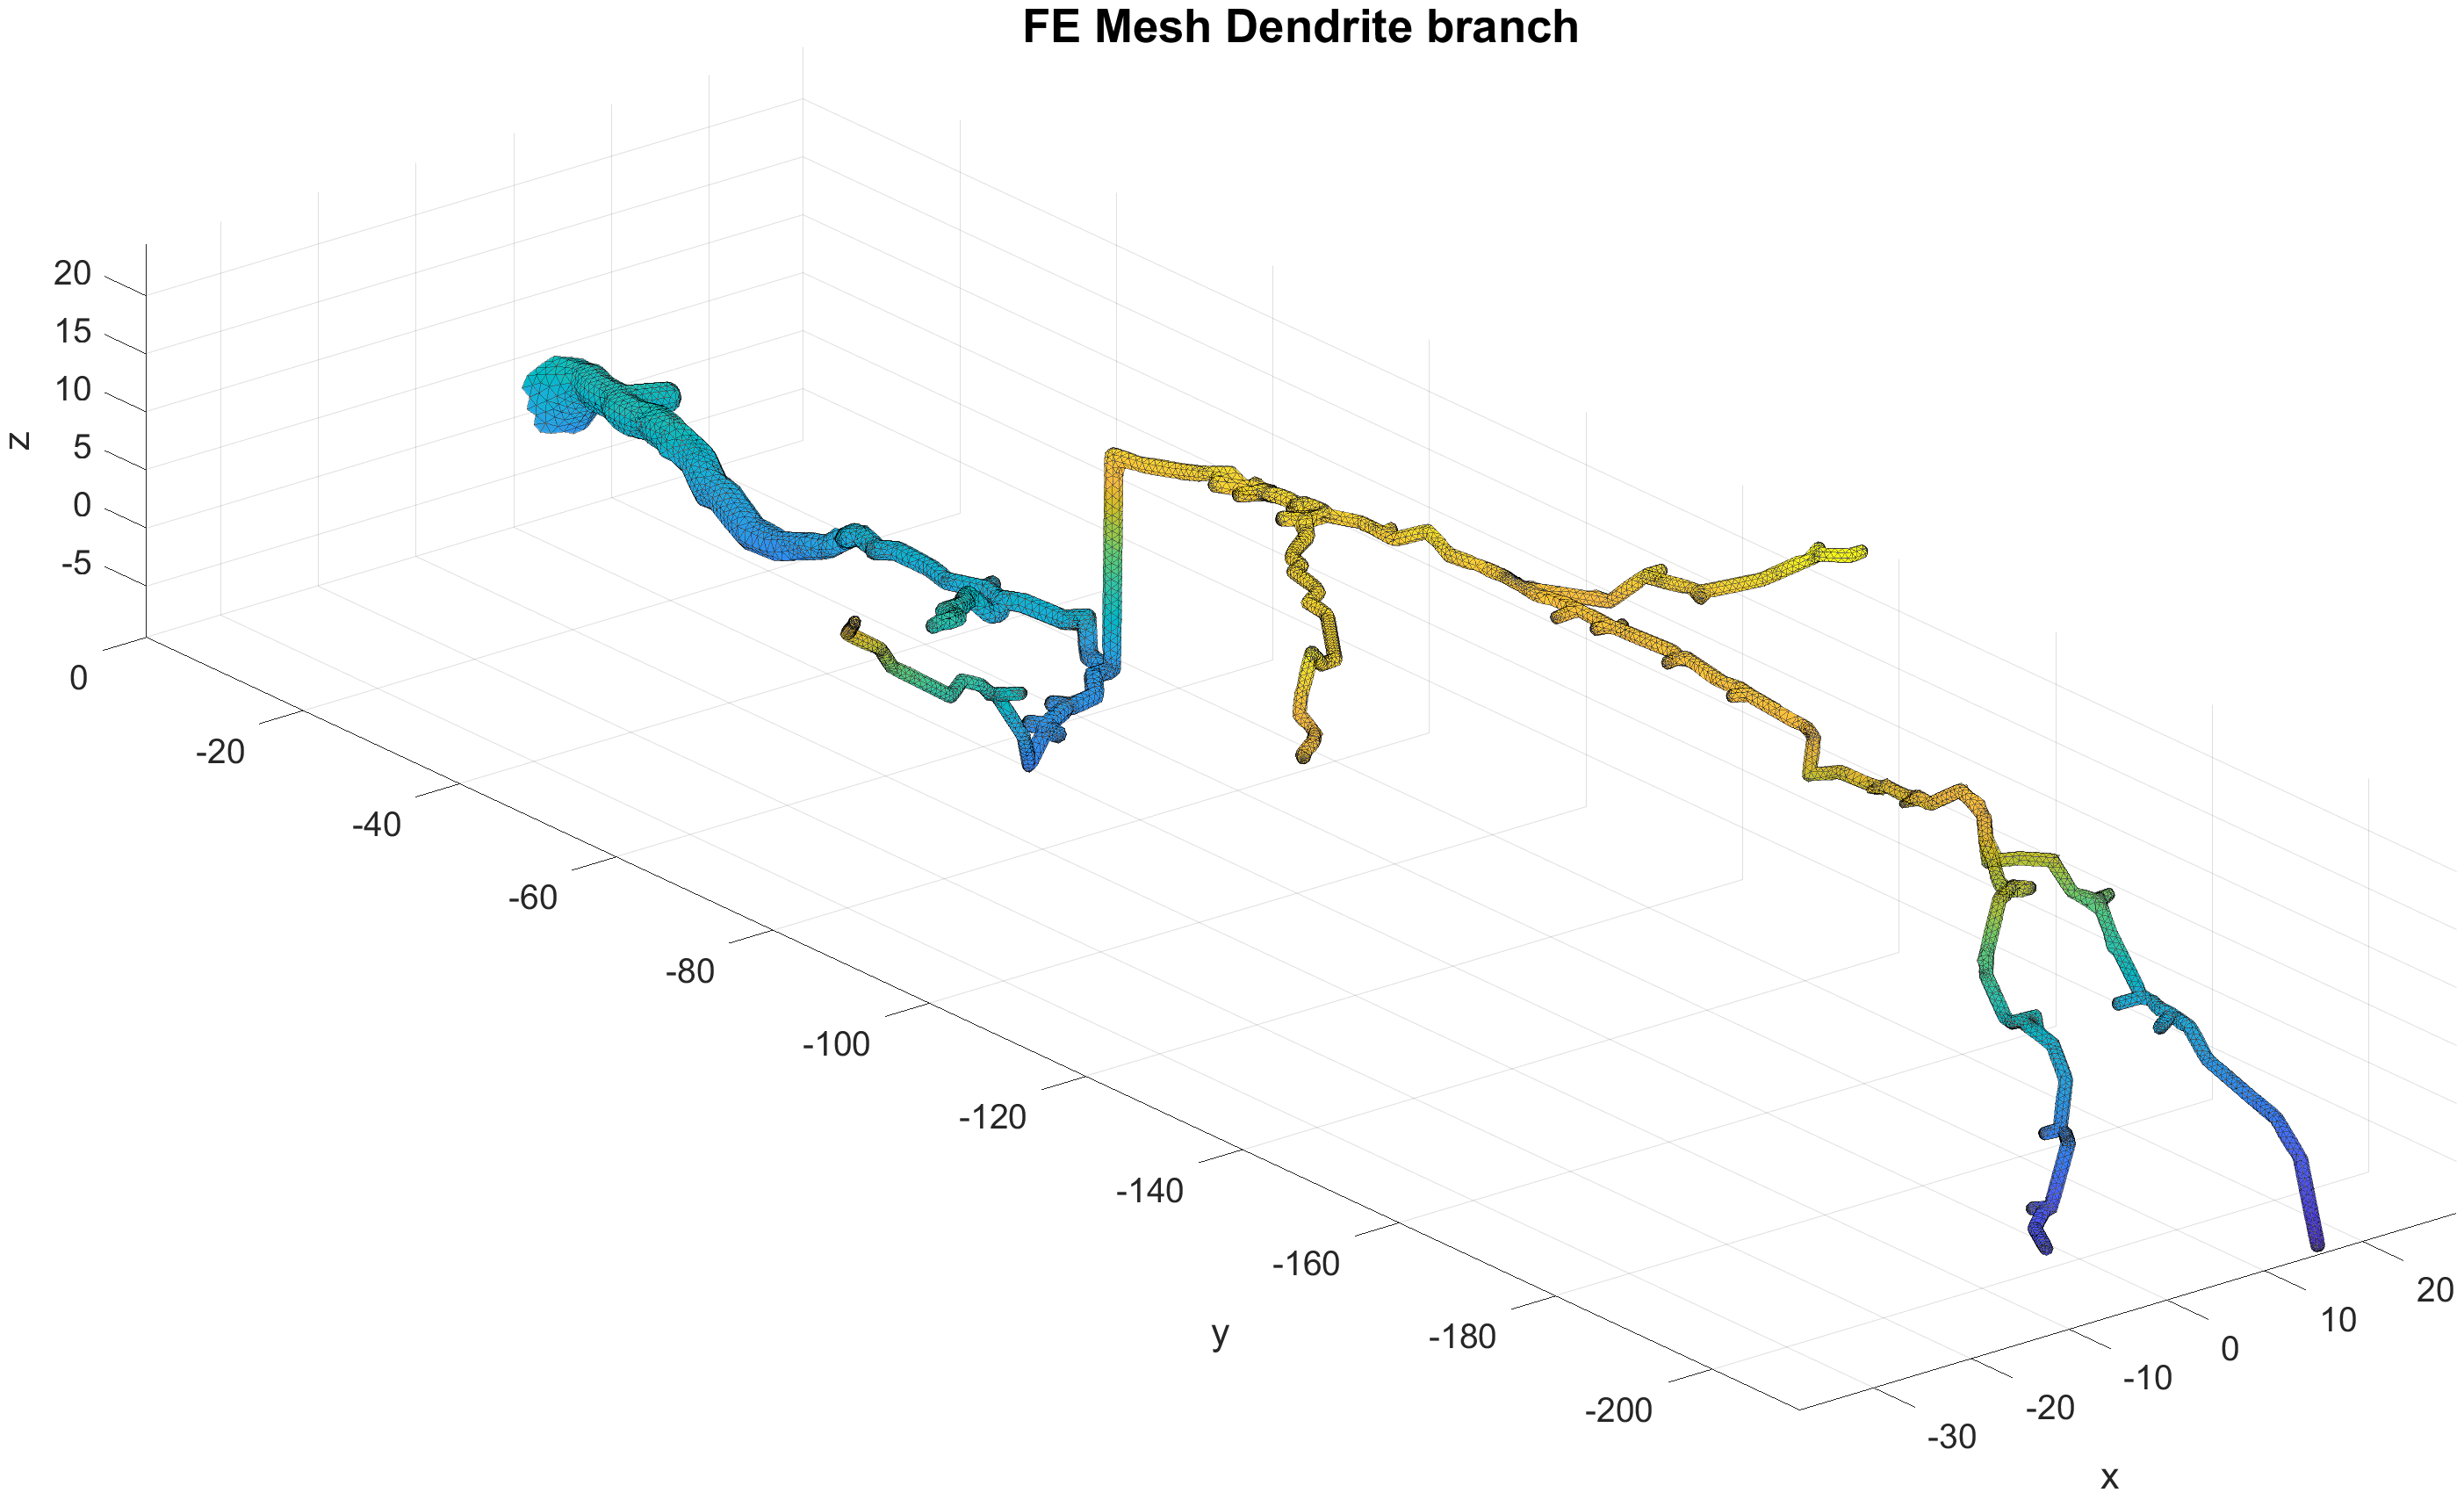
\includegraphics[width=0.49\textwidth]{paper/FEmesh_dendrite}
    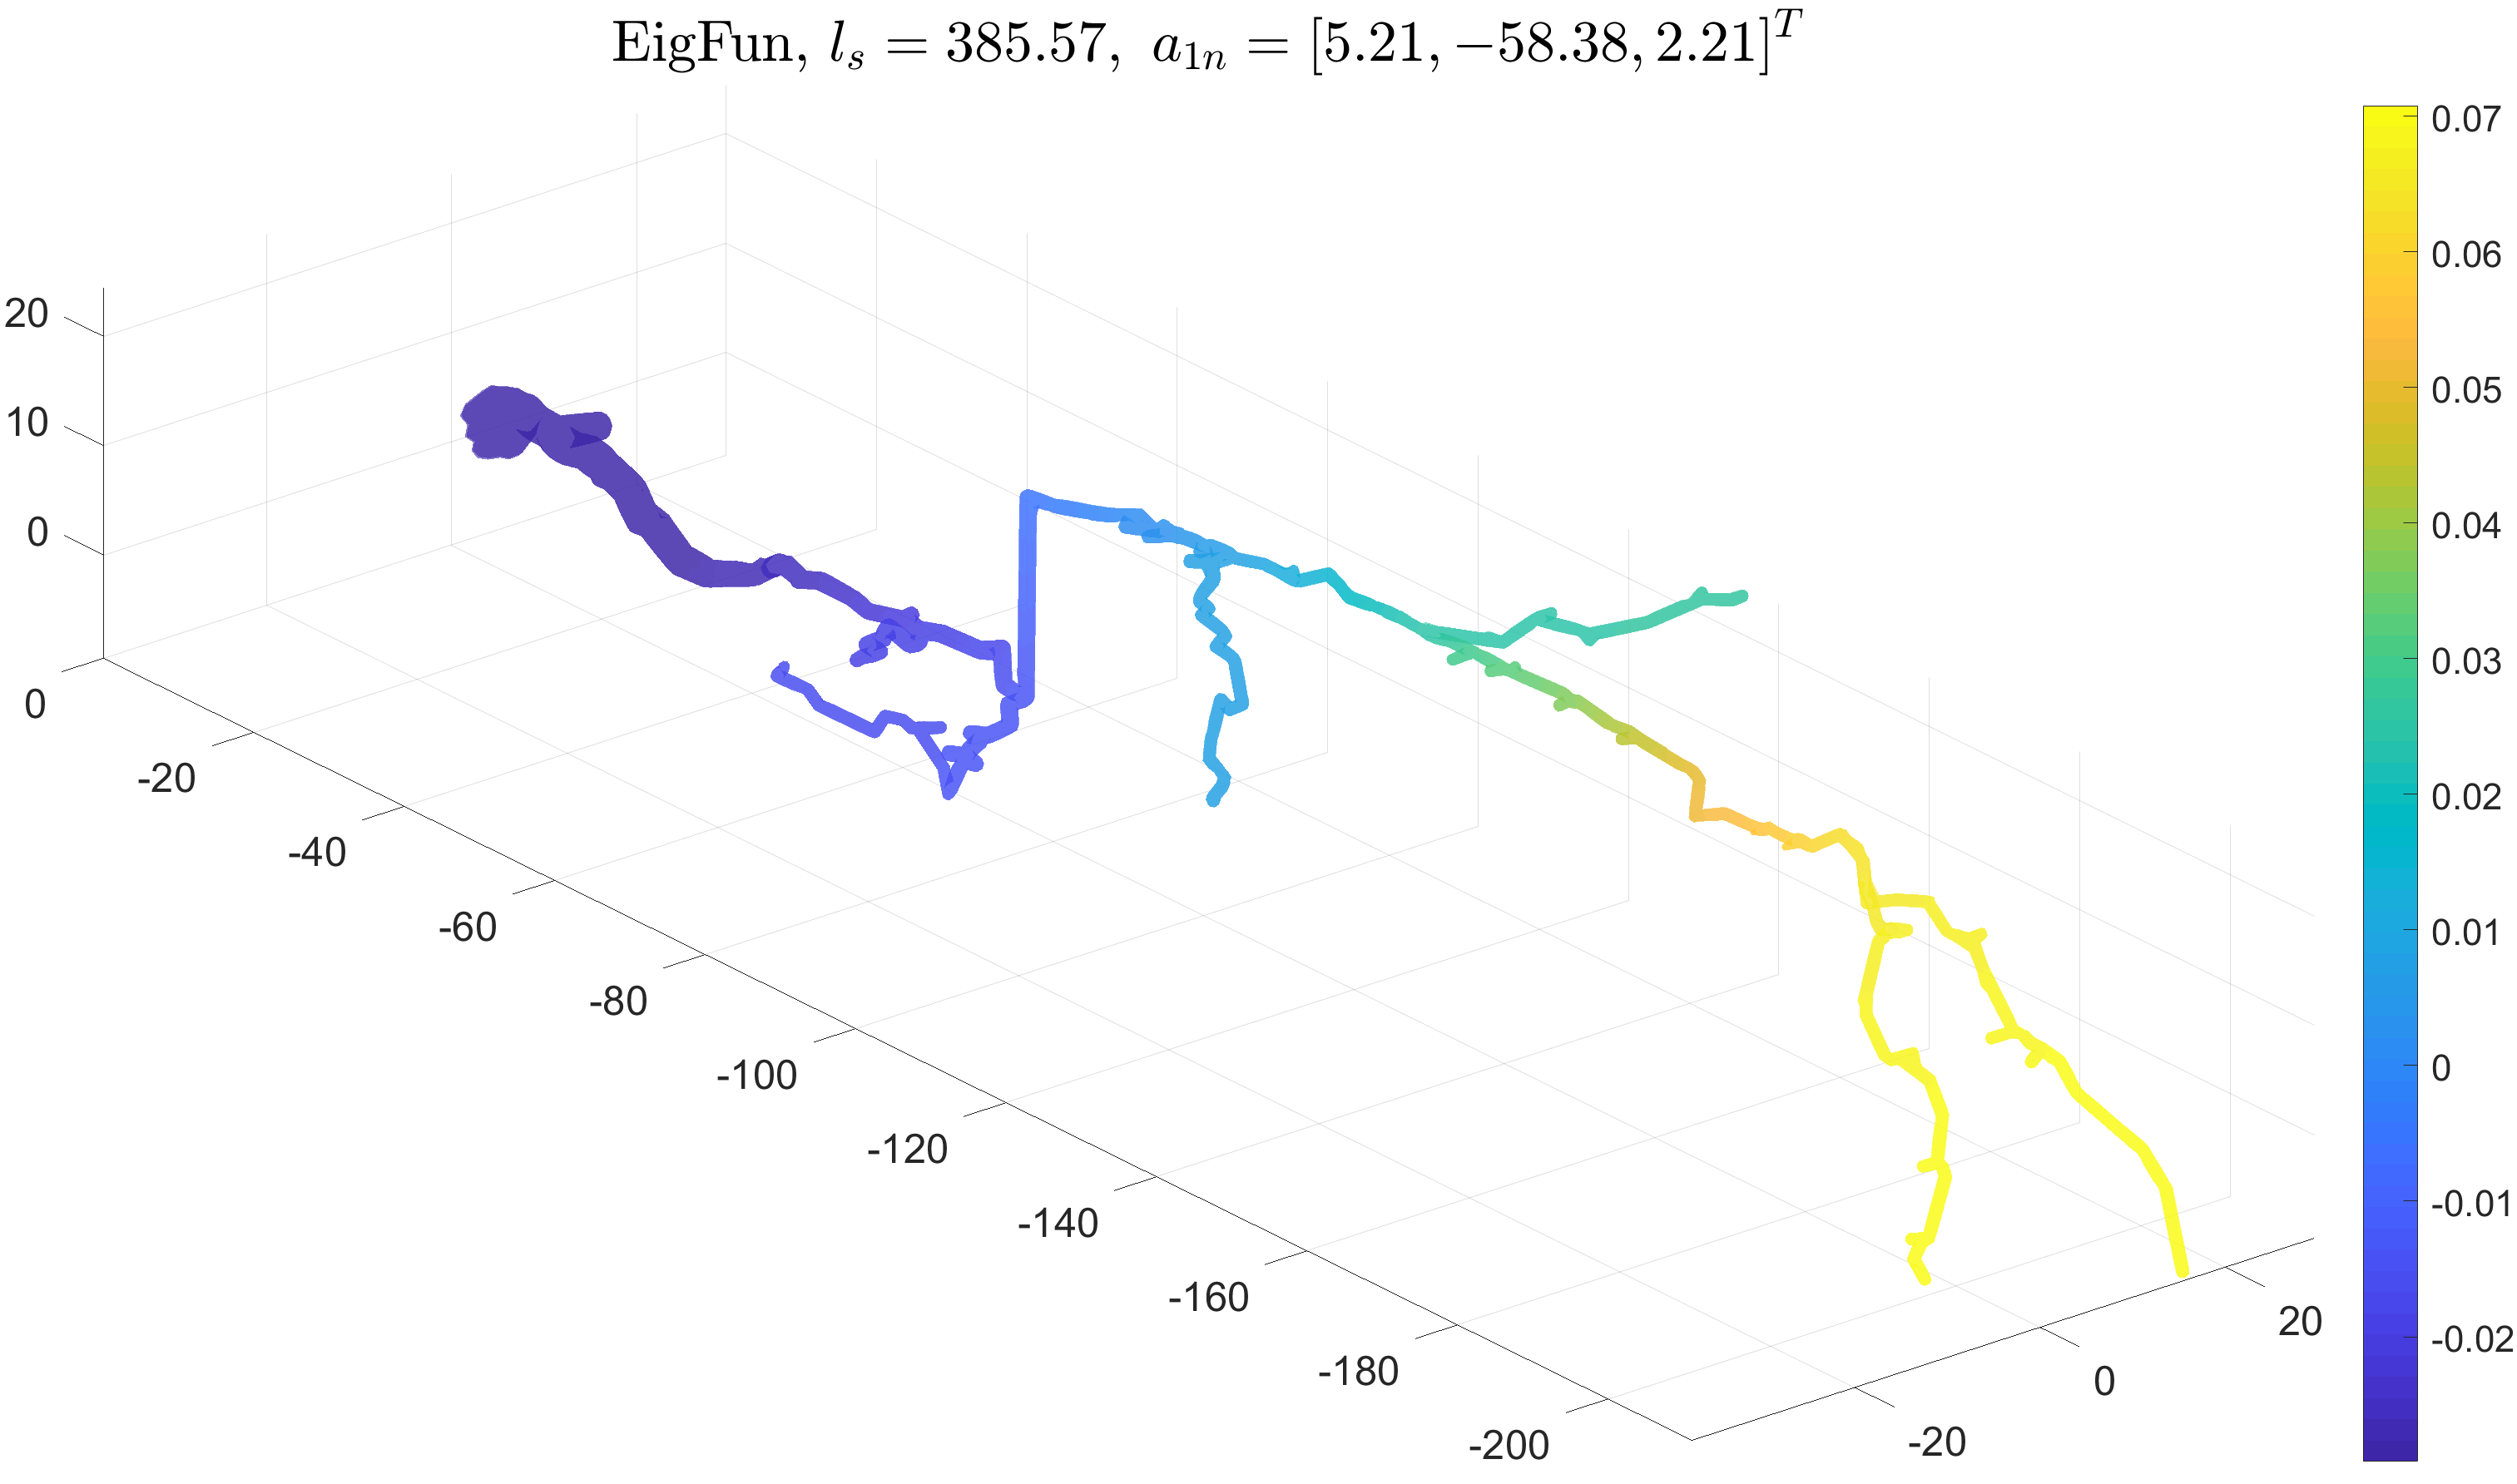
\includegraphics[width=0.49\textwidth]{paper/eigfun}
    \caption{Left: The finite elements mesh of the spindle neuron dendrite branch {\it 03b\_spindle6aACC\_dendrites\_2} (using the command plot\_femesh). Right: The eigenfunction with the associated length scale $L=383.57\lunit$ and the first moments vector $\vec{a}_{1n}=[5.21,-58.38,2.21]^\transpose$ (using the command plot\_field).}
    \label{fig:spindle_dendrite_eigfunc}
\end{figure}

\begin{figure}
    \centering
    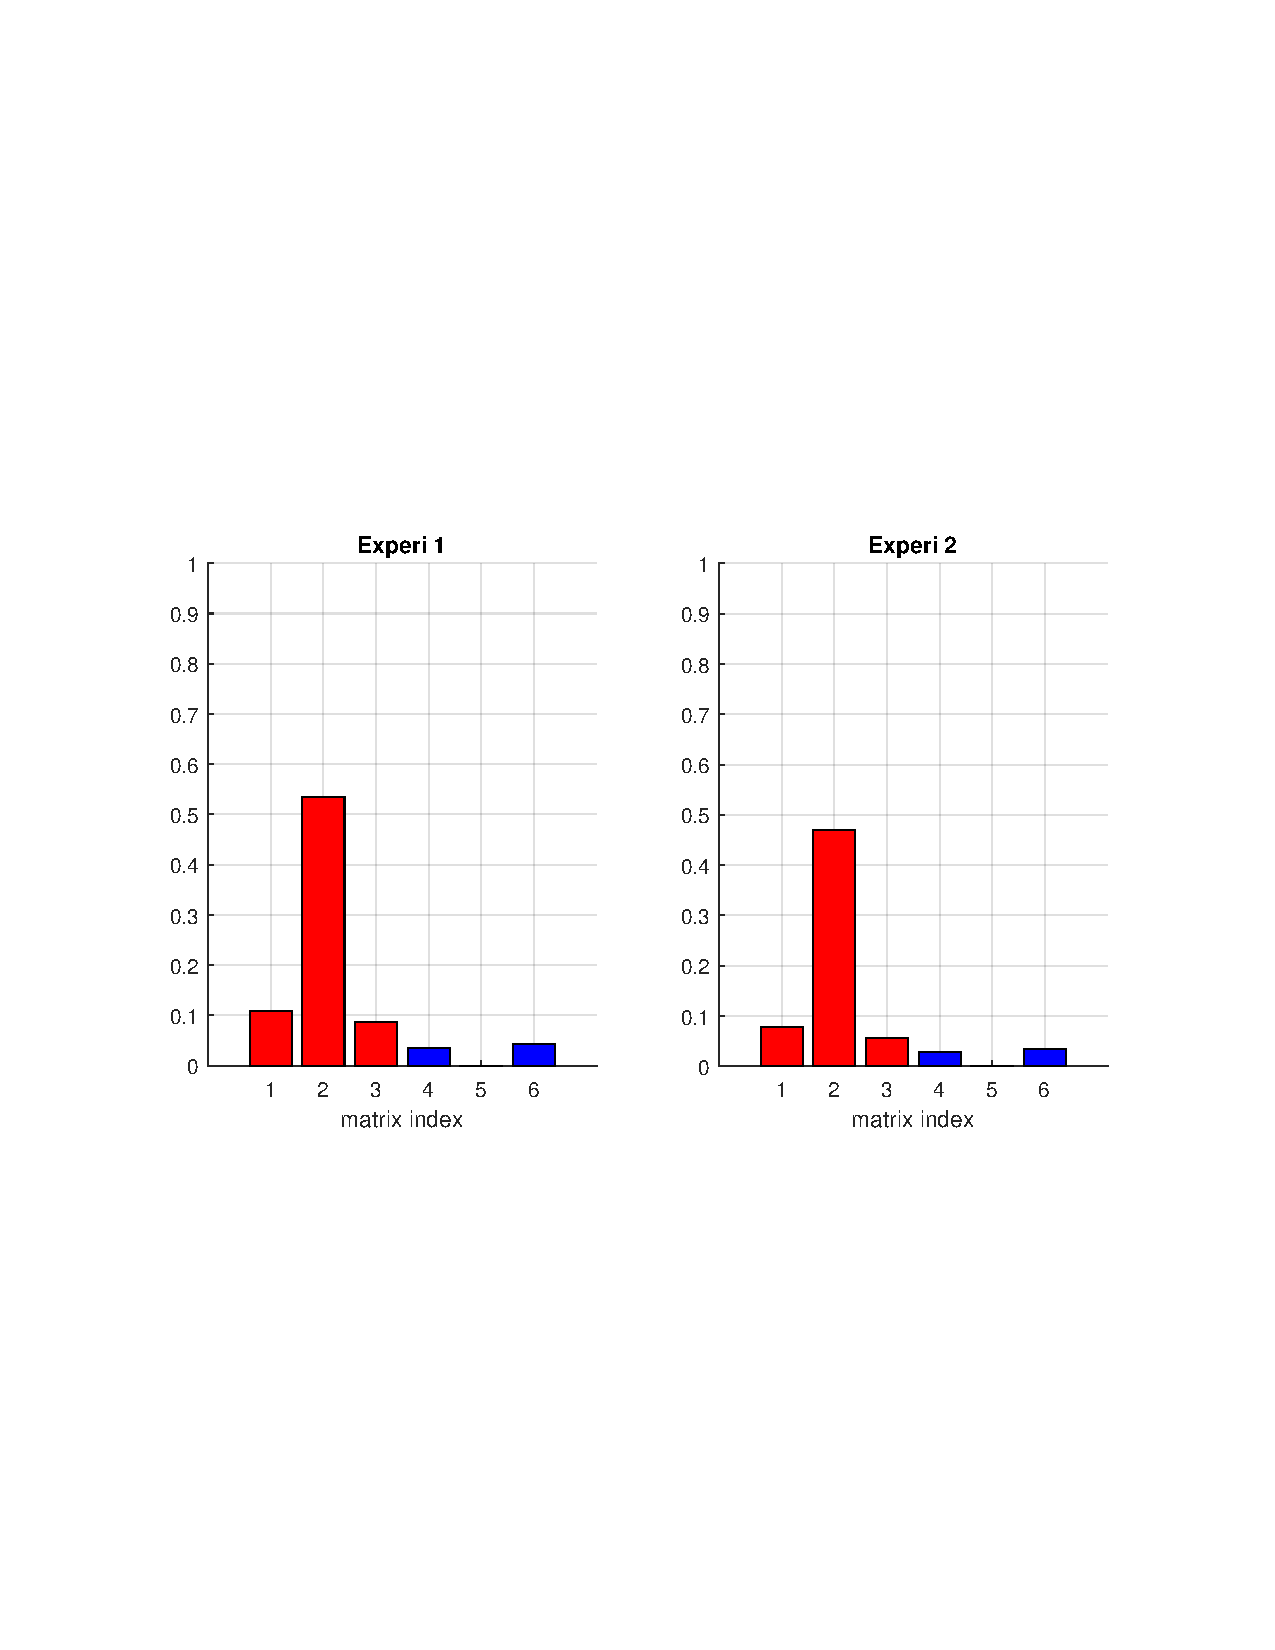
\includegraphics[width=0.8\textwidth]{paper/matrix_index}
    \caption{The 6 entries of the normalized diffusion tensor $\mat{D}^\text{MF}(f)/\Dintr$ for the dendrite branch.
    Indices $1$ to $6$ are in the order of $\{D^{\text{MF}}_{xx}(f),D^{\text{MF}}_{yy}(f),D^{\text{MF}}_{zz}(f),D^{\text{MF}}_{xy}(f),D^{\text{MF}}_{xz}(f),D^{\text{MF}}_{yz}(f)\}/\Dintr$. The diagonal entries of $\mat{D}^\text{MF}(f)/\Dintr$ are shown in red and the off-diagonal entries shown in blue (if non-zero). From left to right: Experiment 1: $f_1$ is PGSE ($\delta=10.6\tunit$, $\Delta=13\tunit$), Experiment 2: $f_2$ is PGSE ($\delta=10.6\tunit$, $\Delta=73\tunit$). (Using the command plot\_diffusion\_tensor).}
    \label{fig:dtensor}
\end{figure}

\begin{figure}
    \centering
    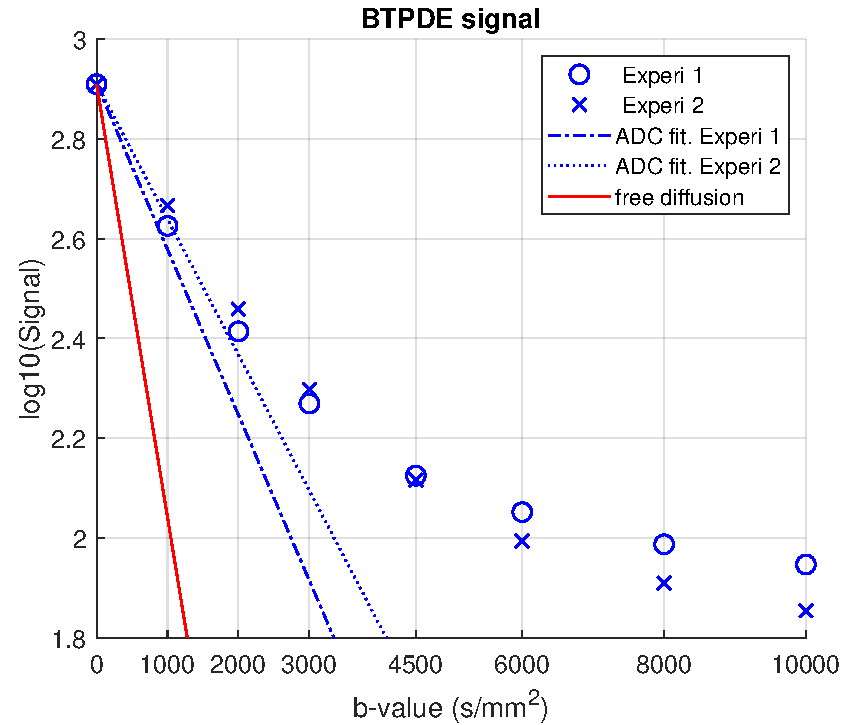
\includegraphics[width=0.4\textwidth]{paper/btpde}
    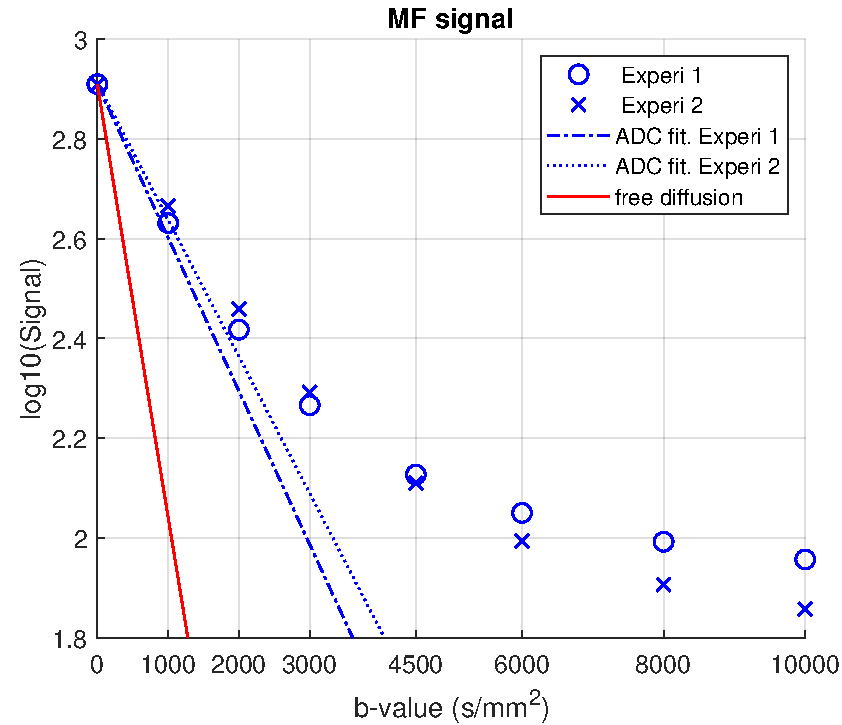
\includegraphics[width=0.4\textwidth]{paper/mf} \\
    \vspace{0.4cm}
    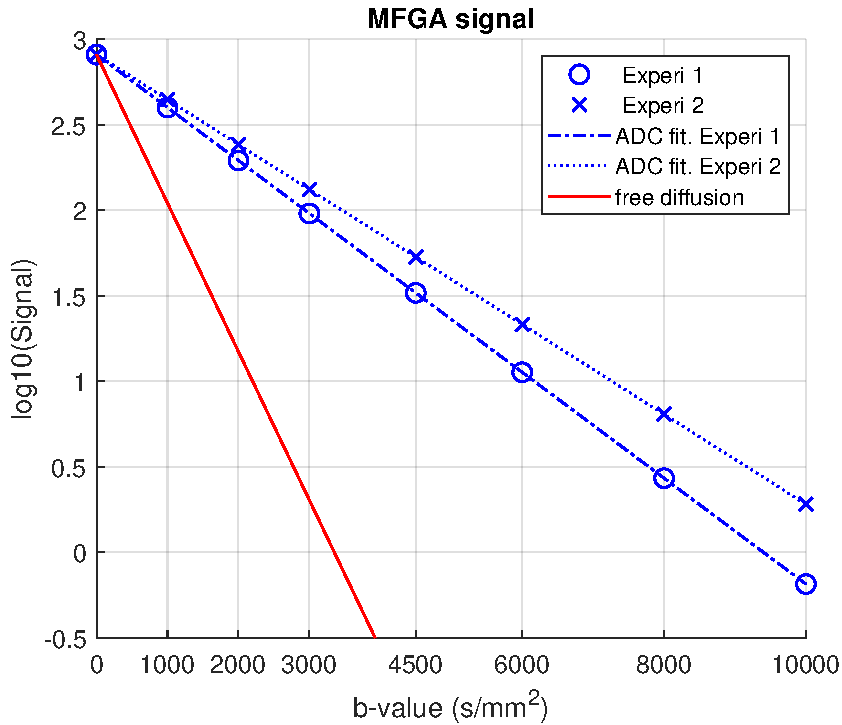
\includegraphics[width=0.4\textwidth]{paper/mfga}
    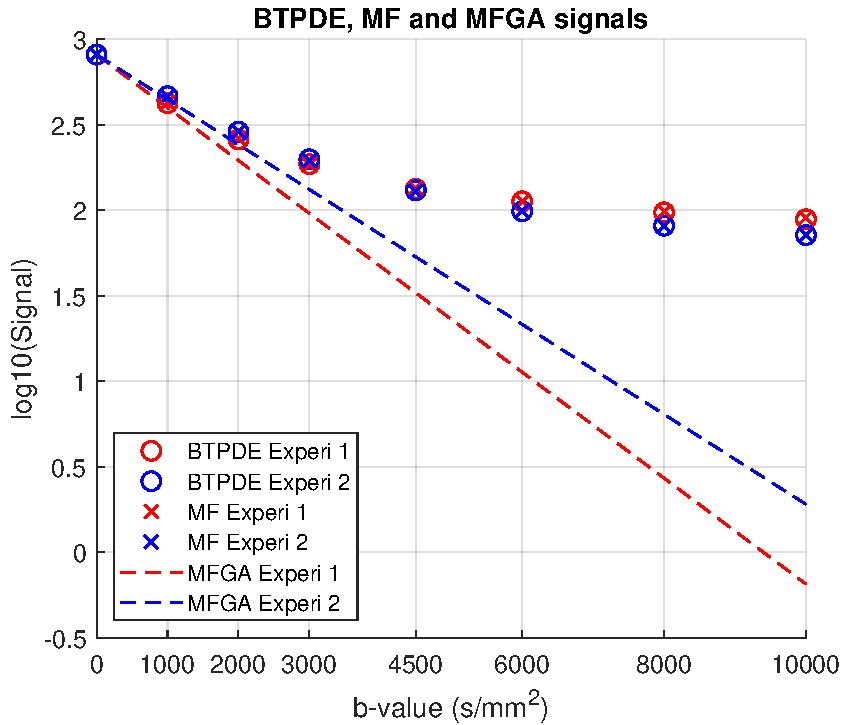
\includegraphics[width=0.4\textwidth]{paper/btpde_mf_mfga}
    \caption{Top left: the BTPDE signals. Top right: the MF signals. Bottom left: the MFGA signals. The markers indicate the values of the simulated signals, the blue lines indicate the ADC fit of those signals, the red line is the signal of free diffusion at the intrinsic diffusion coefficient. Bottom right: the BTPDE, the MF, the MFGA signals plotted together. Experiment 1: $f_1$ is PGSE ($\delta = 10.6\tunit$, $\Delta=13\tunit$), Experiment 2: $f_2$ is PGSE ($\delta=10.6\tunit$, $\Delta=73\tunit$). Diffusion-encoding direction $\vec{u}_{\vec{g}} = (1,1,0)^\transpose / \sqrt{2}$ (using the command plot\_signal).}
    \label{fig:signal_mf}
\end{figure}

\begin{figure}
    \centering
    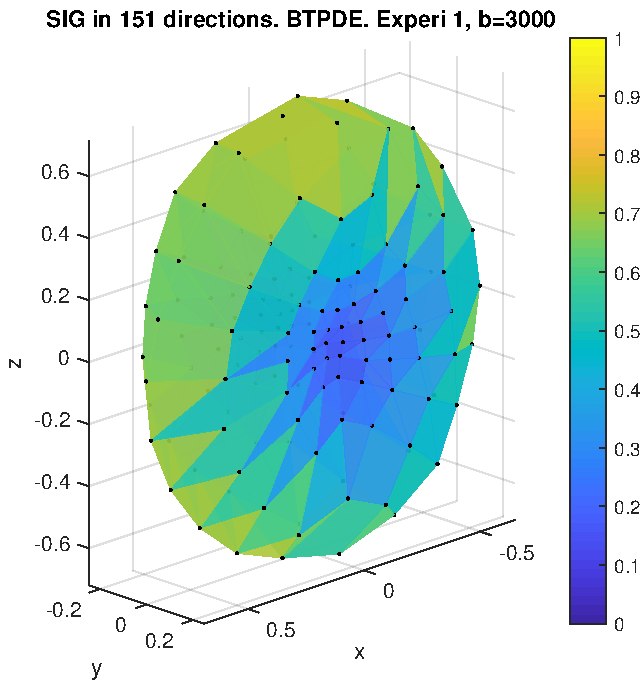
\includegraphics[width=0.3\textwidth]{paper/SIG_BTPDE_151_experi1} \quad \quad
    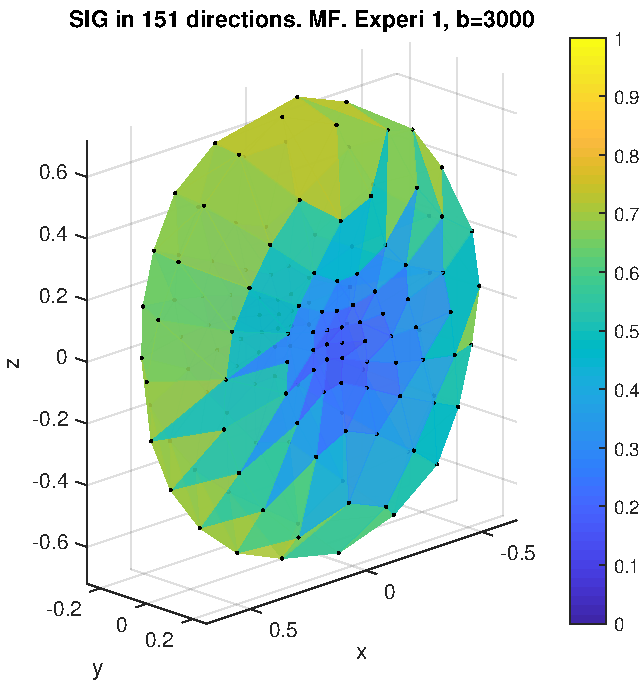
\includegraphics[width=0.3\textwidth]{paper/SIG_MF_151_experi1} \\
    \vspace{0.6cm}
    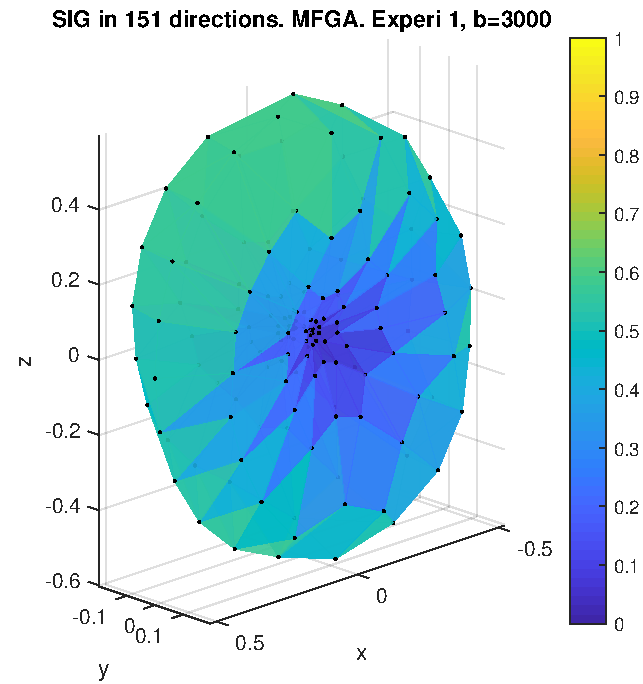
\includegraphics[width=0.3\textwidth]{paper/SIG_MFGA_151_experi1} \quad\quad
    \includegraphics[width=0.3\textwidth]{paper/SIG_MF_900_experi1}
    \caption{Top left: the BTPDE signals, $S^\text{BTPDE}/S_0$, in 151 diffusion-encoding directions. Top right: the MF signals, $S^\text{MF}/S_0$, in 151 diffusion-encoding directions. Bottom left: the MFGA signals, $S^\text{MFGA}/S_0$, in 151 diffusion-encoding directions. Bottom right: the MF signals, $S^\text{MF}/S_0$, in 900 diffusion-encoding directions. The black points are the magnitude of the signal attenuation multiplied by the diffusion-encoding direction. The color indicates the value of the signal attenuation. $b=3000\bunit$, PGSE, $\delta=10.6\tunit$, $\Delta=13\tunit$. (Using the command plot\_hardi).}
    \label{fig:sig_hardi_mf}
\end{figure}



\pagebreak


\bibliographystyle{elsarticle-num}

\bibliography{bibliography/references}

\end{document}
